\documentclass[11pt]{article}
\usepackage{graphics,graphicx}
%\usepackage[dvips]{graphics,graphicx}
\DeclareGraphicsExtensions{.ps,.jpg,.eps,.pdf,.png}
\usepackage{boxedminipage,amsmath,amsfonts}
\usepackage{url}
%\usepackage{secdot}
%\usepackage{natbib}
\usepackage{verbatim}
%\usepackage{moreverb}
\usepackage{enumerate}
\usepackage{makeidx}
\bibliographystyle{plain}
\makeindex

   
%%%%%
% some other macros
\newcommand{\figurepath}{./figures}
\newcommand{\bibpath}{/Users/kmartin/Documents/files/misc}
\newcommand{\figfiletype}{pdf}

%Brad Bell Macros

% Latex macros defined for all the CppAD documentation:
\newcommand{\T}{ {\rm T} }
\newcommand{\R}{ {\bf R} }
\newcommand{\C}{ {\bf C} }
\newcommand{\D}[2]{ \frac{\partial #1}{\partial #2} }
\newcommand{\DD}[3]{ \frac{\partial^2 #1}{\partial #2 \partial #3} }
\newcommand{\Dpow}[2]{ \frac{\partial^{#1}}{\partial  {#2}^{#1}} }
\newcommand{\dpow}[2]{ \frac{ {\rm d}^{#1}}{{\rm d}\, {#2}^{#1}} }

% Define the hangref environment used for the References list:
\newenvironment{hangref}
  {\begin{list}{}{\setlength{\itemsep}{4pt}
  \setlength{\parsep}{0pt}\setlength{\leftmargin}{+\parindent}
  \setlength{\itemindent}{-\parindent}}}{\end{list}}

% Set the page margins to 1 inch all around:
\marginparwidth 0pt\marginparsep 0pt \topskip 0pt\headsep
0pt\headheight 0pt \oddsidemargin 0pt\evensidemargin 0pt
\textwidth 6.5in \topmargin 0pt\textheight 9.0in
\newtheorem{theorem}{Theorem}

   
%%%%Added by Leo%%%%
\newcounter{Fig}
\renewcommand{\theFig}{\arabic{Fig}}
\newcommand{\Fig}[2]{\refstepcounter{Fig} \label{#1}
                     {\small\bf Figure \theFig.} {\small\sl #2 \par}}

\setcounter{topnumber}{3}
\renewcommand{\topfraction}{.9}
\setcounter{bottomnumber}{3}
\renewcommand{\bottomfraction}{.9}
\setcounter{totalnumber}{4}
\renewcommand{\textfraction}{.1}
\setlength{\floatsep}{.25in}
\setlength{\intextsep}{.25in}

\setlength{\fboxrule}{2\fboxrule} \setlength{\fboxsep}{3\fboxsep}

\newcommand{\Sa}{8pt}
\newcommand{\Sb}{0pt}

\renewcommand{\_}{{\char"5F}}
\renewcommand{\{}{{\char"7B}}
\renewcommand{\}}{{\char"7D}}
\renewcommand{\^}{{\char"0D}}

\let\accute= \'
\renewcommand{\'}{{\char"0D}}

\newcommand{\bfit}{\bfseries\itshape}

\newlength{\extopskip} \newlength{\exbottomskip}
\setlength{\exbottomskip}{1\baselineskip}
\addtolength{\exbottomskip}{-5.0pt}
\setlength{\extopskip}{1\exbottomskip}
\addtolength{\extopskip}{-1\parskip}

\newenvironment{Example}{\vspace{1\extopskip}\noindent\hspace*{2em}
                         \frenchspacing\small
                         \tt\begin{tabular}{@{}l@{}}}{
                         \end{tabular}\\[1\exbottomskip]}

\newcommand{\Titem}{\item[$\triangleright$]}
\newcommand{\Ditem}{\item[$\diamond$]}

\newenvironment{Itemize}{\begin{quote}\normalsize
   \baselineskip 20pt plus .3pt minus .1pt \begin{itemize}}
   {\end{itemize}\end{quote}}
   % Set path to folder containing figures
\newcommand{\FigureFolder}{figures}

\newif\ifknitro \knitrofalse    % change to \knitrotrue once we get knitro connected again
\newif\ifipopt  \ipopttrue      % change to \ipopttrue  once we get the build problems sorted out


% We use a number of URLs that point to software downloads. These locations are forever changing,
% and maintaining them is a nightmare. All the URLs are gathered here, so that we can at least
% get away with making changes only once...
\newcommand{\UrlAmpl}{http://www.ampl.com}
\newcommand{\UrlAmplSandia}{http://netlib.sandia.gov/ampl/}
\newcommand{\UrlAmplSolvers}{http://netlib.sandia.gov/cgi-bin/netlib/netlibfiles.tar?filename=netlib/ampl/solvers}
\newcommand{\UrlApacheFileupload}{http://jakarta.apache.org/commons/fileupload/}
\newcommand{\UrlBlas}{ftp://www.netlib.org/blas/blas.tgz}
\newcommand{\UrlBonmin}{http://projects.coin-or.org/Bonmin}
\newcommand{\UrlBuildtools}{http://projects.coin-or.org/BuildTools}
\newcommand{\UrlCbc}{http://projects.coin-or.org/Cbc}
\newcommand{\UrlCgl}{http://projects.coin-or.org/Cgl}
\newcommand{\UrlCl}{http://www.microsoft.com/express/download/\#webInstall}
\newcommand{\UrlClp}{http://projects.coin-or.org/Clp}
\newcommand{\UrlCoinConfig}{https://projects.coin-or.org/BuildTools/wiki/user-configure\#PreparingtheCompilation}
\newcommand{\UrlCoinConfigure}{http://projects.coin-or.org/BuildTools/wiki/user-configure\#CommandLineArgumentsforconfigure}
\newcommand{\UrlCoinCygwin}{http://projects.coin-or.org/BuildTools/wiki/current-issues}
\newcommand{\UrlCoinDownload}{http://projects.coin-or.org/BuildTools/wiki/user-download\#DownloadingtheSourceCode}
\newcommand{\UrlCoinNames}{https://projects.coin-or.org/CoinBinary/wiki/ArchiveNamingConventions}
\newcommand{\UrlCoinProjects}{http://www.coin-or.org/projects/}
\newcommand{\UrlCoinUtils}{http://projects.coin-or.org/CoinUtils}
\newcommand{\UrlCouenne}{http://projects.coin-or.org/Couenne}
\newcommand{\UrlCpl}{http://www.ibm.com/developerworks/library/os-cpl.html}
\newcommand{\UrlCplex}{http://www.ilog.com/products/cplex/}
\newcommand{\UrlCppad}{http://projects.coin-or.org/CppAD}
\newcommand{\UrlCygwinMake}{http://www.cmake.org/files/cygwin/make.exe}
\newcommand{\UrlCygwinSetup}{http://www.cygwin.com/setup.exe}
\newcommand{\UrlDoxygen}{http://www.doxygen.org}
\newcommand{\UrlDylp}{http://projects.coin-or.org/DyLP}
\newcommand{\UrlFToC}{http://www.netlib.org/f2c}
\newcommand{\UrlFToCBin}{http://www.netlib.org/f2c/mswin/}
\newcommand{\UrlFToCZip}{http://www.netlib.org/f2c/libf2c.zip}
\newcommand{\UrlGgs}{http://www.g95.org}
\newcommand{\UrlGamslinks}{https://projects.coin-or.org/svn/GAMSlinks/trunk}
\newcommand{\UrlGcc}{http://gcc.gnu.org}
\newcommand{\UrlGfortran}{http://gcc.gnu.org/fortran/}
\newcommand{\UrlGlpk}{http://www.gnu.org/software/glpk/}
\newcommand{\UrlGlpkDownload}{ftp://ftp.gnu.org/gnu/glpk/glpk-4.42.tar.gz}
\newcommand{\UrlHsl}{http://www.cse.scitech.ac.uk/nag/hsl/}
\newcommand{\UrlIpopt}{http://projects.coin-or.org/Ipopt}
\newcommand{\UrlIpoptDoc}{https://projects.coin-or.org/Ipopt/browser/stable/3.5/Ipopt/doc/documentation.pdf?format=raw}
\newcommand{\UrlIpoptDocxiii}{http://www.coin-or.org/Ipopt/documentation/node13.html}
\newcommand{\UrlKippFileupload}{http://gsbkip.chicagogsb.edu/os/fileupload.html}
\newcommand{\UrlKnitro}{http://www.ziena.com/}
\newcommand{\UrlKnitroMan}{http://www.ziena.com/docs/knitroman.pdf}
\newcommand{\UrlLapack}{ftp://www.netlib.org/lapack/lapack-lite-3.1.0.tgz}
\newcommand{\UrlMingw}{http://downloads.sourceforge.net/mingw/MSYS-1.0.11.exe?modtime=1079444447\&big\_mirror=1}
\newcommand{\UrlMsys}{http://sourceforge.net/project/showfiles.php?group\_id=2435}
\newcommand{\UrlMsysBinary}{http://downloads.sourceforge.net/mingw/bash-3.1-MSYS-1.0.11-1.tar.bz2?modtime=1195140582\&big\_mirror=1}
\newcommand{\UrlMsysAddIns}{http://sourceforge.net/project/showfiles.php?group\_id=2435\&package\_id=67879}
\newcommand{\UrlMsysBison}{bison-2.3-MSYS-1.0.11-1.tar.bz2}
\newcommand{\UrlMsysFlex}{flex-2.5.33-MSYS-1.0.11-1.tar.bz2}
\newcommand{\UrlMsysRegex}{regex-0.12-MSYS-1.0.11-1.tar.bz2}
\newcommand{\UrlNewticket}{http://projects.coin-or.org/OS/newticket}
\newcommand{\UrlNightlyBuild}{https://projects.coin-or.org/TestTools/wiki/NightlyBuildInAction}
\newcommand{\UrlOs}{http://www.optimizationservices.org}
\newcommand{\UrlOsBinaries}{http://www.coin-or.org/download/binary/OS/}
\newcommand{\UrlOsCommon}{https://projects.coin-or.org/svn/OS/branches/OScpp/OSCommon}
\newcommand{\UrlOsDoxygen}{http://www.coin-or.org/OS/doxydoc/html/index.html}
\newcommand{\UrlOsi}{http://projects.coin-or.org/Osi}
\newcommand{\UrlOsJava}{https://projects.coin-or.org/svn/OS/branches/OSjava}
\newcommand{\UrlOsRelease}{https://projects.coin-or.org/svn/OS/releases/2.1.0}
\newcommand{\UrlOsStable}{https://projects.coin-or.org/svn/OS/stable/2.1}
\newcommand{\UrlOsTarball}{http://www.coin-or.org/download/source/OS/}
\newcommand{\UrlOsWin}{https://projects.coin-or.org/CoinBinary/browser/binary/OS}
\newcommand{\UrlParinclinear}{http://www.coin-or.org/OS/parincLinear.osil}
\newcommand{\UrlSdk}{http://www.microsoft.com/downloads/details.aspx?FamilyID=E6E1C3DF-A74F-4207-8586-711EBE331CDC\&displaylang=en}
\newcommand{\UrlSvn}{http://subversion.tigris.org}
\newcommand{\UrlSymphony}{http://projects.coin-or.org/SYMPHONY}
\newcommand{\UrlTomcat}{http://tomcat.apache.org/}
\newcommand{\UrlTortoiseSvn}{http://tortoisesvn.tigris.org}
\newcommand{\UrlTrac}{http://projects.coin-or.org/OS}
\newcommand{\UrlUsingTrac}{http://www.coin-or.org/usingTrac.html}
\newcommand{\UrlVol}{http://projects.coin-or.org/Vol}
\newcommand{\UrlWget}{http://www.christopherlewis.com/WGet/WGetFiles.htm}
\newcommand{\UrlWgetBinary}{http://www.christopherlewis.com/WGet/wget-1.11.4b.zip}

% Current software versions
\newcommand{\GlpkVer}{4.42}
\newcommand{\OSstable}{2.1}
\newcommand{\OSrelease}{2.1.0}
\newcommand{\OStrunk}{3139}
\newcommand{\MsysVer}{1.0.11}
\newcommand{\MsysFile}{bash-3.1-MSYS-1.0.11}



\begin{document}

%Some cross-referencing index entries (to be expanded as needed)
\index{ASL|see{AMPL Solver Library (ASL)}}
\index{HSL|see{Harwell Subroutine Library (HSL)}}
\index{nl files|see{AMPL nl format}}
\index{Bonmin@{\tt Bonmin}|see{COIN-OR projects, {\tt Bonmin}}}
\index{BuildTools@{\tt BuildTools}|see{COIN-OR projects, {\tt BuildTools}}}
\index{Cbc@{\tt Cbc}|see{COIN-OR projects, {\tt Cbc}}}
\index{Cgl@{\tt Cgl}|see{COIN-OR projects, {\tt Cgl}}}
\index{Clp@{\tt Clp}|see{COIN-OR projects, {\tt Clp}}}
%\index{Configuration Manager|see{Microsoft Visual Studio, Configuration Manager}}
\index{Couenne@{\tt Couenne}|see{COIN-OR projects, {\tt Couenne}}}
\index{CppAD@{\tt CppAD}|see{COIN-OR projects, {\tt CppAD}}}
\index{CoinUtils@{\tt CoinUtils}|see{COIN-OR projects, {\tt CoinUtils}}}
%\index{Debug configuration|see{Microsoft Visual Studio, {\tt Debug} configuration}}
\index{DyLP@{\tt DyLP}|see{COIN-OR projects, {\tt DyLP}}}
\index{Ipopt@{\tt Ipopt}|see{COIN-OR projects, {\tt Ipopt}}}
\index{Osi@{\tt Osi}|see{COIN-OR projects, {\tt Osi}}}
%\index{Release configuration|see{Microsoft Visual Studio, {\tt Release} configuration}}
%\index{Release-plus configuration|see{Microsoft Visual Studio, {\tt Release-plus} configuration}}
\index{SYMPHONY@{\tt SYMPHONY}|see{COIN-OR projects, {\tt SYMPHONY}}}
\index{Vol@{\tt Vol}|see{COIN-OR projects, {\tt Vol}}}

\title{Optimization Services \OSstable\ User's Manual }
\vskip 2in
\author{Horand Gassmann, Jun Ma,  Kipp Martin, and Wayne Sheng}
\maketitle

\begin{abstract}
This is the User's Manual for the Optimization Services (OS) project.  The objective of OS is to provide a
general framework consisting of a set of standards for representing optimization instances, results,
solver options, and communication between clients and solvers in a distributed environment using Web Services.
This COIN-OR\index{COIN-OR} project provides C++ and Java source code for libraries and executable programs that 
implement OS standards.   The OS library includes a robust solver and modeling language interface (API) for linear,
nonlinear and other types of optimization problems.   Also included is the C++ source code for a  command line
executable {\tt OSSolverService}\index{OSSolverService@{\tt OSSolverService}}  for reading problem instances 
(OSiL format\index{OSiL}, nl format\index{AMPL nl format}, MPS format\index{MPS format}) and
calling a solver either locally or on a remote server.  Finally,  both Java\index{Java} source code and a Java {\tt war} 
file are provided for users who wish to set up a solver service on a server running Apache Tomcat\index{Apache Tomcat}.
See the Optimization Services home page {\tt\UrlOs} and the COIN-OR Trac page\index{Trac system} {\tt\UrlTrac} for 
more information.
\end{abstract}


\newpage
\tableofcontents
\listoffigures
\listoftables
\hyphenation{com-plex-Type}
\hyphenation{GAMS-links}

 

%\noindent\hrulefill
\newpage

\section{The Optimization Services (OS) Project}

The objective of Optimization Services (OS) is to provide a general framework consisting of a set of standards
for representing optimization instances, results, solver options, and communication between clients and solvers
in a distributed environment using Web Services. This COIN-OR project provides source code for libraries and
executable programs that implement OS standards.  See the COIN-OR Trac page {\tt\UrlTrac}\index{Trac system}
or the Optimization Services Home Page {\tt\UrlOs}\index{Optimization Services} for more information.

Like other COIN-OR projects, OS has a versioning system that ensures end users some degree of stability 
and a stable upgrade path as project development continues. The current stable version of OS is \OSstable, 
and the current stable release is \OSrelease\index{OS project!stable release}, based on trunk version~\OStrunk.

The OS project provides the following:

\begin{enumerate}
\item{}  A set of XML\index{XML} based standards for representing optimization instances (OSiL)\index{OSiL}, 
optimization results (OSrL)\index{OSrL}, and optimization solver options (OSoL)\index{OSoL}. 
There are other standards, but these are the main ones. 
The schemas for these standards are described in Section~\ref{section:schemadescriptions}.


\item{}  Open source libraries  that support and implement many of the standards.

\item{}  A robust solver and modeling language interface (API) for linear and nonlinear optimization problems.
Corresponding to the OSiL problem instance representation there is an in-memory object,
{\tt OSInstance}\index{OSInstance@{\tt OSInstance}},
along with a collection of  {\tt get()},   {\tt set()}, and {\tt calculate()} methods for accessing and creating
problem instances. This is a very general API for linear, integer, and nonlinear programs.
Extensions for other major types of optimization problems are also in the works. Any modeling language that can
produce OSiL can easily communicate with any solver that uses the OSInstance API.   
The {\tt OSInstance}\index{OSInstance@{\tt OSInstance}} object
is described in more detail in Section~\ref{section:osinstanceAPI}. The nonlinear part of the API is based on the
COIN-OR project CppAD\index{COIN-OR projects!CppAD@{\tt CppAD}} by Brad Bell ({\tt\UrlCppad}) but is written 
in a very general manner and could be used with other algorithmic differentiation packages. More detail on 
algorithmic differentiation is provided in Section~\ref{section:ad}.


\item{}  A  command line executable {\tt OSSolverService}\index{OSSolverService@{\tt OSSolverService}}  for reading
problem instances (OSiL format\index{OSiL}, AMPL  nl format\index{AMPL nl format},  
MPS format\index{MPS format}) and calling a solver either locally or on a remote server.
This is described in Section~\ref{section:ossolverservice}.


\item{} Utilities that convert AMPL nl files  and MPS files into the OSiL XML format.
This is described in Section~\ref{section:osmodelinterfaces}.


\item{}  Standards that facilitate the communication between clients and optimization solvers using Web Services.
In  Section~\ref{section:osagent} we describe the {\tt OSAgent}\index{OSAgent@{\tt OSAgent}} part of the OS library
that is used to create Web Services SOAP\index{SOAP protocol} packages with OSiL instances and contact a server for 
solution.

\item{}  An executable program {\tt OSAmplClient}\index{OSAmplClient@{\tt OSAmplClient}} that is designed to work with 
the AMPL\index{AMPL} modeling language. The {\tt OSAmplClient} appears as a ``solver'' to AMPL and, based on options 
given in AMPL, contacts solvers either remotely or locally to solve instances created in AMPL. This is described in
Section~\ref{section:amplclient}.

\item{}  Server software that works with Apache Tomcat\index{Apache Tomcat} and Apache Axis\index{Apache Axis}.
This software uses Web Services technology and acts as middleware between the client that creates the instance
and the  solver on the server that optimizes the instance and returns the result. This is illustrated in
Section~\ref{section:tomcat}.

\item{}  A lightweight version of the project, {\tt OSCommon},\index{OSCommon@{\tt OSCommon}} for modeling language and 
solver developers who want to use OS API, readers and writers, without the overhead of other COIN-OR projects or any 
third-party software. For information on how to download {\tt OSCommon} see Section~\ref{section:oslite}.
\end{enumerate}


\section{Quick Roadmap}\label{section:roadmap}

If you want to:

\begin{itemize}
\item Download the OS source code or binaries -- see Section~\ref{section:download}.

\item Download just the OS API, readers and writers -- see Section~\ref{section:oslite}.

\item Build the OS project from the source code -- see Section~\ref{section:build}.

\item Use the OS library to build model instances or use solver APIs -- see Sections \ref{section:osmodelinterfaces},
\ref{section:ossolverinterfaces} and~\ref{section:osinstanceAPI}.

\item Use the OSSolverService to read files in nl\index{AMPL nl format}, OSiL\index{OSiL}, 
or MPS format\index{MPS format} and call a solver locally or remotely -- see Section~\ref{section:ossolverservice}.


\item Use AMPL\index{AMPL} to solve problems either locally or remotely
with a COIN-OR solver, Cplex\index{cplex@{\tt cplex}},
GLPK\index{GLPK@{\tt GLPK}}, \ifknitro Knitro\index{knitro}, \fi
or LINDO\index{LINDO} -- see Section~\ref{section:amplclient}.

\item Use GAMS\index{GAMS} to solve problems either locally or remotely -- see Section~\ref{section:gamslinks}.

\item Build a remote solver service using Apache Tomcat\index{Apache Tomcat} -- see Section~\ref{section:tomcat}.

\item Use MATLAB\index{MATLAB} to generate problem instances in OSiL format and call a solver either remotely or locally
 -- see Section~\ref{section:usingmatlab}.

\item Use the OS library for algorithmic differentiation\index{Algorithmic differentiation} (in conjunction with 
COIN-OR CppAD)\index{COIN-OR projects!CppAD@{\tt CppAD}} -- see Section~\ref{section:ad}.

\item Use modeling languages to generate model instances in OSiL format -- see Section \ref{section:modellang}.
\end{itemize}


\section{Downloading the OS Project}\label{section:download}

The OS project is an open-source project  with source code under the Common Public License~(CPL)%
\index{Common Public License (CPL)}.
See~{\tt\UrlCpl}.  This project was initially created by Robert Fourer, Jun Ma, and Kipp Martin.
The code has been written primarily by  Horand Gassmann,   Jun Ma,  and Kipp Martin.    
Horand Gassmann,  Jun Ma,  and Kipp Martin are the COIN-OR project leaders and active developers for the OS project.
%Below we describe different methods for obtaining the binaries and C++ source code.
Most users will only be interested in obtaining the binaries, which we describe 
in Section~\ref{section:obtainingbinaries}. The remaining sections of this chapter deal with obtaining the 
source code for the project, which will be of interest mostly to developers.




\subsection{Obtaining the Binaries}\label{section:obtainingbinaries}

If the user does not wish to compile source code, the OS library, OSSolverService executable
and Tomcat server software configuration are available in binary format for some operating systems.     
The repository is at {\tt\UrlOsBinaries}\index{Downloading!binaries}. Unlike the source code described 
in Section~\ref{section:downloadwithsvn}, the binary files are not subject to version control and can be
downloaded using an ordinary browser. If binaries are not provided for a particular operating system,
it may be possible to build them from the source code. Since the source is under version control, 
this requires svn. (See Sections \ref{section:svn}, \ref{section:downloadwithsvn} and~\ref{section:build}.

The binary distribution for the OS library and executables follows the following naming convention:


\begin{verbatim}
OS-version_number-platform-compiler-build_options.tgz (zip)
\end{verbatim}
For example, OS  Release 2.1.0 compiled with the Intel 9.1 compiler on an Intel 32-bit Linux system is:
\begin{verbatim}
OS-2.1.0-linux-x86-icc9.1.tgz
\end{verbatim}

For more detail on the naming convention and examples see:

\medskip
\noindent{\tt\UrlCoinNames}
\medskip

After unpacking the {\tt tgz} or {\tt zip} archives, the following folders are available.
\begin{itemize}

\item[] {\bf bin --} this directory has the executables {\tt OSSolverService}\index{OSSolverService@{\tt OSSolverService}} 
and {\tt OSAmplClient}\index{OSAmplClient@{\tt OSAmplClient}}.

\item[]  {\bf include --} the header files that are necessary necessary  in order to link against the OS library.

\item[] {\bf lib --} the libraries that are necessary for creating applications that use the OS library.

\item[] {\bf  share --} license and author information for all the projects used by the OS project.
\end{itemize}



Files are also provided for an Apache Tomcat\index{Apache Tomcat} Web server along with the associated Web service
that can
read SOAP \index{SOAP protocol} envelopes with model instances in OSiL\index{OSiL} format and/or options in 
OSoL\index{OSoL} format, call the {\tt OSSolverService}\index{OSSolverService@{\tt OSSolverService}},
and return the optimization result in OSrL\index{OSrL} format.
The naming convention\index{file naming conventions} for the server binary is
\begin{verbatim}
OS-server-version_number.tgz (.zip)
\end{verbatim}
For example, the files associated with  OS server release 2.0.0 are in the binary distribution
\begin{verbatim}
OS-server-2.0.0.tgz
\end{verbatim}
There is no platform information given since the server and related binaries were written in Java\index{Java}.
The details and use of this distribution are described in Section~\ref{section:tomcat}.

Finally for Windows users we provide Visual Studio \index{Microsoft Visual Studio} project files (and supporting
libraries and header files) for building projects based on the OS library and libraries used by the OS project.
The binary for this is named
\begin{verbatim}
OS-version_number-VisualStudio.zip
\end{verbatim}
For example, the necessary files associated with  OS  stable\index{OS project!stable release} \OSstable\ are in the binary 
distribution
\begin{verbatim}
OS-2.1-VisualStudio.zip
\end{verbatim}
The binaries provided are based on Visual Studio Express 2008.  See Section \ref{section:vsexamples} for more detail.

\subsection{Auxiliary Software for Working with the OS Project} \label{section:auxiliarydownloads}

Compiling and modifying the OS project source\index{OS project!source code} code can be a daunting task,
made somewhat easier by the inclusion of configure scripts\index{configure!scripts} and makefiles
in the distribution of the source. However, additional software packages are
sometimes needed or convenient, especially on Windows.
We collect in this section a number of recommended packages that we ourselves use in the development
and maintenance of the code.

\subsubsection{Subversion (SVN)}\label{section:svn}

The Subversion\index{Subversion} version control package is used to obtain the C++ source code\index{OS project!source code}.
Users with Unix operating systems will most likely have a command line svn client.  If an svn client is not present,
see~{\tt\UrlSvn} to download an svn client.   For Windows users we recommend the
svn client  TortoiseSVN.  (See~{\tt\UrlTortoiseSvn}.) Upon installation the TortoiseSVN client is integrated within the
Windows  Explorer.

\subsubsection{wget}\label{section:wget}
Certain third-party software (see Section~\ref{section:otherthirdparty}) is available in source form but is not
contained in the OS project distribution. Scripts are included to download this code using the
{\tt wget}\index{wget@{\tt wget}} executable.


%The {\tt wget} executable is used by the scripts, {\tt get.ASL},
%{\tt get.Blas}, etc. in the corresponding third-party subdirectories
%and makes it easy to download the software.
A Windows version of {\tt wget} is available at

%\begin{verbatim}
%http://www.christopherlewis.com/WGet/WGetFiles.htm
%\end{verbatim}

\medskip
\noindent{\tt\UrlWgetBinary}
\medskip

%Windows users are advised to download only the binary found in
%
%\begin{verbatim}
%http://www.christopherlewis.com/WGet/wget-1.10.2b.zip
%\end{verbatim}
%or the beta version of the new release at
%\begin{verbatim}
%http://www.christopherlewis.com/WGet/wget-1.11-beta-1b.zip
%\end{verbatim}


There is no need to rebuild the code locally, which relies on several levels of other software.

\subsubsection{Windows development platform}\label{section:windowsdevelopment}
A development platform is essential for users on Windows. OS Project provides support for Microsoft Visual Studio
(see Section~\ref{section:msvs}) and several unix emulators, including Cygwin (Section~\ref{section:cygwin}),
MinGW (Section~\ref{section:mingw}) and MSYS (Section~\ref{section:msys}). Download instructions for all of these
packages are included in the sections indicated.

\subsubsection{C++ compiler}\label{section:cpp}
A C++ compiler\index{C++ compiler} is needed to compile the OS source\index{OS project!source code}. This should be present 
under all unix\index{Unix} installations. If no C++ compiler is available on the system, the free {\tt gcc}\index{gcc} 
compiler can be downloaded from {\tt\UrlGcc}.

Microsoft Visual Studio can be configured with the Microsoft {\tt cl}\index{cl compiler@{\tt cl} compiler} compiler, 
which also works under MSYS\index{MSYS}. MinGW\index{MinGW} and Cygwin\index{Cygwin} are normally configured 
with the Gnu compiler collection ({\tt gcc}), although they can also be used with the {\tt cl} compiler. 
However, extreme care is needed if the last option is followed. {\tt gcc} and {\tt cl} have very different 
header files, and it is important to set up the {\tt \$PATH}\index{PATH@{\tt \$PATH}} variable correctly 
in order not to confuse the header files. 
In our experience, best results are achieved with the minimal unix-like installation, MSYS, and the 
Microsoft {\tt cl} compiler.

\subsubsection{Fortran Compiler}\label{section:fortran}
The COIN-OR project Ipopt\index{COIN-OR projects!Ipopt@{\tt Ipopt}} (see Section~\ref{section:ipopt}) and several of 
the third-party software described in Section~\ref{section:otherthirdparty} include Fortran\index{Fortran} subroutines, 
which must be compiled with a Fortran compiler if the user wants to include these projects in the build. A free 
Fortran~95 compiler
can be downloaded from {\tt\UrlGgs}. For Fortran~77 code (which includes the Blas\index{Blas},
HSL\index{Harwell Subroutine Library (HSL)} and Lapack\index{Lapack} projects --- but {\bf not} Mumps\index{Mumps}) 
it might be sufficient to download the {\tt f2c}\index{f2c@{\tt f2c}} translator
which turns Fortran~77 code into code that can subsequently be fed into a C compiler.
The {\tt f2c} translator and the {\tt f2c} runtime library can be downloaded from {\tt\UrlFToC}.
Further details are available in the file {\tt BuildTools/compile\_f2c/INSTALL}, which is part of the OS distribution.

\subsubsection{{\tt flex} and {\tt bison} }\label{section:flex}
Users who want to edit the source code in the parsers described in
Section~\ref{section:osparsers} will need the additional  tools
{\tt flex}\index{flex@{\tt flex}} and {\tt bison}\index{bison@{\tt bison}}.  These can be downloaded from

%\begin{verbatim}
%http://sourceforge.net/project/showfiles.php?group\_id=2435
%\end{verbatim}

\medskip
\noindent{\tt\UrlMsysAddIns}
\medskip

\noindent and are listed at the Web site as

\begin{verbatim}
bison-2.3-MSYS-1.0.11-1
flex-2.5.33-MSYS-1.0.11-1
regex-0.12-MSYS-1.0.11-1
\end{verbatim}
The last file contains an important DLL, msys-regex-0.dll, without which {\tt flex} will not start.

\subsubsection{doxygen }\label{section:doxygen}
Doxygen\index{Doxygen}  ({\tt\UrlDoxygen}) is a document production system that can be used to prepare documentation
for the OS project and related software. For details, see Section~\ref{section:documentation}.

 
\subsection{Obtaining OS Source Code Using Subversion (SVN)}\label{section:downloadwithsvn}

For the rest of this documentation, we assume that  the name of the root directory
of the OS project\index{OS project!root directory} distribution is {\tt COIN-OS}.  
The {\tt COIN-OS} directory structure is illustrated in Figure~\ref{figure:osprojectrootdir}.
OS source code is mainly contained inside of the OS subdirectory. Other first level subdirectories are mostly
external projects (COIN-OR or third-party) that the OS project depends on.


\begin{figure}
\centering
%\includegraphics[scale=0.7]{\figurepath/OSProjectRootDirectory.png}
\includegraphics[scale=0.7]{./figures/OSProjectRootDirectory.png}
\caption{The OS distribution root directory.}
\label{figure:osprojectrootdir}
\end{figure}

\medskip

For Users on a Unix system\index{Downloading!subversion!unix}\index{Unix} such as Linux, Solaris, Mac OS X, etc., 
the source code is obtained as follows. In a command window execute:

%\begin{verbatim}
%svn co https://projects.coin-or.org/svn/OS/releases/1.1.0 COIN-OS
%\end{verbatim}

\medskip
\noindent{\tt svn co \UrlOsRelease\ COIN-OS}
\medskip

It is possible that on some systems you may get a message such as:
\begin{verbatim}
Error validating server certificate for 'https://projects.coin-or.org:443':
 - The certificate is not issued by a trusted authority. Use the
   fingerprint to validate the certificate manually!
Certificate information:
 - Hostname: projects.coin-or.org
 - Valid: from Jun 10 22:51:18 2007 GMT until Jun 15 21:00:28 2009 GMT
 - Issuer: 07969287, http://certificates.godaddy.com/repository, GoDaddy.com, Inc.,
Scottsdale, Arizona, US
 - Fingerprint: f7:26:0f:bb:e1:94:a5:23:7f:5c:cb:c3:9a:c4:74:51:e5:c7:4d:29
(R)eject, accept (t)emporarily or accept (p)ermanently?
\end{verbatim}

If so, select {\tt (p)} and you should not get this message again.

\medskip

For more information on downloading the OS project or other COIN-OR projects using SVN\index{SVN} see

\nopagebreak\medskip\nopagebreak
\noindent{\tt\UrlCoinDownload}.
\medskip

\vskip 8pt

On Windows\index{Downloading!subversion!Windows}\index{Microsoft Windows} with TortoiseSVN\index{TortoiseSVN}, 
create a directory {\tt COIN-OS}
in the desired location and right-click on this directory. Select the menu item {\tt SVN Checkout ...}
and in the textbox ``{\tt URL of Repository}'' give the URL for the version of the OS project you wish
to check out, for instance, 

\medskip
\noindent{\tt\UrlOsStable}.
\medskip


Now build the project as described in  Section~\ref{section:build}.

\medskip

The Java\index{Java} source code for  setting up a solver service with Apache Tomcat\index{Apache Tomcat} is 
checked out as follows:
%\begin{verbatim}
%svn co https://projects.coin-or.org/svn/OS/branches/OSjava  OSJava
%\end{verbatim}

\medskip
\noindent{\tt svn co \UrlOsJava\ OSJava}
\medskip

For more detail on running a Tomcat solver service  see  Section~\ref{section:tomcat}.








\subsection{Obtaining the OS Source Code From a Tarball or Zip File}\label{section:getTarBalls}

The OS source code can also be obtained from either a  tarball\index{Downloading!tarball} or
zip\index{Downloading!zip file} file.  This may be preferred for users who are not managing other
COIN-OR projects and wish to only work with periodic release versions of the code.  In order to obtain the code
from a Tarball or Zip file do the following.

\vskip 8pt

\begin{enumerate}[{\bf Step 1:}]

\item{}
In a browser open the link {\tt\UrlOsTarball}.  Listed at this page are files in the format:

\begin{verbatim}
OS-release_number.tgz
OS-release_number.zip
\end{verbatim}

\vskip 8pt

\item{}
Click on either the {\tt tgz} or {\tt zip} file and download to the desired directory.

\vskip 8pt

\item{}
Unpack the files. For {\tt tgz} do the following at the command line:
\begin{verbatim}
gunzip OS-release_number.tgz
tar -xvf OS-release_number.tar
\end{verbatim}

Windows users should be  able to double-click on the file {\tt OS-release\_number.zip} and have the directory unpacked.

\vskip 8pt

\item{}
(optional) Move the folder {\tt OS-release\_number} to the desired location and rename it to {\tt COIN-OS}.
\end{enumerate}


Now build the project as described in  Section~\ref{section:build}.







\subsection{Obtaining source for the OS Project API} \label{section:oslite}
The OS project is very extensive and relies on many other COIN-OR projects\index{COIN-OR}.
This may not be desirable for modeling language and solver developers who just wish to use the OS API
in conjunction with their modeling language or solver.  Hence there is also an ``OS lite'' download
that consists of all the code for the OS API and for reading and writing instance and solution files.
%
%We refer to this version of the project as {\tt OSCommon}\index{OSCommon@{\tt OSCommon}} and the code
%for this project is synched with the corresponding stable and release versions of the code.
%For example, to get Stable 1.1 of {\tt OSCommon} use the svn command
%\begin{verbatim}
%svn co https://projects.coin-or.org/svn/OS/stable/OSCommon1.1  OSCommon
%\end{verbatim}
%
We refer to this version of the project as {\tt OSCommon}\index{OSCommon@{\tt OSCommon}}. 
To get the current version of {\tt OSCommon} use the svn\index{SVN} command

\medskip
\noindent{\tt svn co \UrlOsCommon\ OSCommon}


\section{Building and Testing the OS Project}\label{section:build}


Once the OS source code is obtained, the OS libraries, {\tt OSSolverService}\index{OSSolverService@{\tt OSSolverService}} 
executable, and test examples can be built.
We describe how to do this on Unix/Linux\index{Unix} systems (see Section~\ref{section:unixbuilds})
and on Windows\index{Microsoft Windows} (see Section~\ref{section:windowsinstall}).

\subsection{Building the OS Project on Unix/Linux Systems}\label{section:unixbuilds}

In order to build the OS project on Unix/Linux systems do the following.

\vskip 8pt

\begin{enumerate}[{\bf Step 1:}]
\item{} Connect to the OS distribution root directory ({\tt COIN-OS} in Figure~\ref{figure:osprojectrootdir}).

\vskip 8pt



\item{} \label{itemize:unixbuilds} Run the configure script that will generate the makefiles.
If you are running on a machine with a Fortran\index{Fortran} 95 compiler present (e.g., {\tt gfortran}), and you have
previously downloaded the third-party software packages {\tt BLAS}\index{Blas} and {\tt Mumps}\index{Mumps}
(see Section~\ref{section:ipopt}), run the command

\begin{verbatim}
./configure
\end{verbatim}
\index{configure}

\noindent otherwise use

\begin{verbatim}
./configure  COIN_SKIP_PROJECTS="Ipopt Bonmin"
\end{verbatim}
\index{COIN_SKIP_PROJECTS@{\tt COIN\_SKIP\_PROJECTS}}
as COIN-OR's {\tt Ipopt}\index{COIN-OR projects!Ipopt@{\tt Ipopt}} and
{\tt Bonmin}\index{COIN-OR projects!Bonmin@{\tt Bonmin}}
projects currently use Fortran to compile some of its dependent libraries.

\vskip 8pt
\noindent {\bf Notes:}

\begin{itemize}
\item If {\tt gfortran} is not present and you  wish to build the nonlinear solver {\tt Ipopt} see the instructions 
in Section~\ref{section:ipopt}.

\item When using {\tt configure} you may wish to use the {\tt -C} option. This
instructs {\tt configure} to use a cache file, {\tt config.cache}\index{configure!cache file}, to speed up configuration
by remembering and reusing the results of tests already performed.

\item For more information and options on the {\tt ./configure} script see

\noindent{\footnotesize {\tt\UrlCoinConfig}.}

\item You  cannot apply  {\tt COIN\_SKIP\_PROJECTS}\index{COIN_SKIP_PROJECTS@{\tt COIN\_SKIP\_PROJECTS}} to 
{\tt Cbc}\index{COIN-OR projects!Cbc@{\tt Cbc}}, 
{\tt Clp}\index{COIN-OR projects!Clp@{\tt Clp}}, 
{\tt Cgl}\index{COIN-OR projects!Cgl@{\tt Cgl}}, 
{\tt CoinUtils}\index{COIN-OR projects!CoinUtils@{\tt CoinUtils}}, 
%{\tt CppAD}\index{COIN-OR projects!CppAD@{\tt CppAD}}, 
or {\tt Osi}\index{COIN-OR projects!Osi@{\tt Osi}}.
These projects must be present.
\end{itemize}



\item{}  Run the make files.

\begin{verbatim}
make
\end{verbatim}

\item{} Run the {\tt unitTest}\index{unitTest@{\tt unitTest}}.

\begin{verbatim}
make test
\end{verbatim}

\ifknitro
Depending upon which third-party software you have installed, the result of running the {\tt unitTest} should look
something like (we have included the third-party solvers LINDO\index{LINDO} and Knitro\index{Knitro} in the test 
results below; they are not part of the default build):


{\small
\begin{verbatim}
HERE ARE THE UNIT TEST RESULTS:

Solved problem avion2.osil with Ipopt
Solved problem HS071.osil with Ipopt
Solved problem rosenbrockmod.osil with Ipopt
Solved problem parincQuadratic.osil with Ipopt
Solved problem parincLinear.osil with Ipopt
Solved problem callBack.osil with Ipopt
Solved problem callBackRowMajor.osil with Ipopt
Solved problem parincLinear.osil with Clp
Solved problem p0033.osil with Cbc
Solved problem rosenbrockmod.osil with Knitro
Solved problem callBackTest.osil with Knitro
Solved problem parincQuadratic.osil with Knitro
Solved problem HS071_NLP.osil with Knitro
Solved problem p0033.osil with SYMPHONY
Solved problem parincLinear.osil with DyLP
Solved problem volumeTest.osil with Vol
Solved problem p0033.osil with GLPK
Solved problem lindoapiaddins.osil with Lindo
Solved problem rosenbrockmod.osil with Lindo
Solved problem parincQuadratic.osil with Lindo
Solved problem wayneQuadratic.osil with Lindo
Test the MPS -> OSiL converter on parinc.mps using Cbc
Test the AMPL nl -> OSiL converter on hs71.nl using LINDO
Test a problem written in b64 and then converted to OSInstance
Successful test of OSiL parser on problem parincLinear.osil
Successful test of OSrL parser on problem parincLinear.osrl
Successful test of prefix and postfix conversion routines on problem rosenbrockmod.osil
Successful test of all of the nonlinear operators on file testOperators.osil
Successful test of AD gradient and Hessian calculations on problem CppADTestLag.osil

All tests completed successfully
\end{verbatim}
}
\else
Depending upon which third-party software you have installed, the result of running the {\tt unitTest}\index{OS project!unit test}
should look
something like (we have included the third-party solver LINDO\index{LINDO} in the test results below; it is not
part of the default build):


{\small
\begin{verbatim}
HERE ARE THE UNIT TEST RESULTS:

Solved problem avion2.osil with Ipopt
Solved problem HS071.osil with Ipopt
Solved problem rosenbrockmod.osil with Ipopt
Solved problem parincQuadratic.osil with Ipopt
Solved problem parincLinear.osil with Ipopt
Solved problem callBack.osil with Ipopt
Solved problem callBackRowMajor.osil with Ipopt
Solved problem parincLinear.osil with Clp
Solved problem p0033.osil with Cbc
Solved problem p0033.osil with SYMPHONY
Solved problem parincLinear.osil with DyLP
Solved problem volumeTest.osil with Vol
Solved problem p0033.osil with GLPK
Solved problem lindoapiaddins.osil with Lindo
Solved problem rosenbrockmod.osil with Lindo
Solved problem parincQuadratic.osil with Lindo
Solved problem wayneQuadratic.osil with Lindo
Test the MPS -> OSiL converter on parinc.mps using Cbc
Test the AMPL nl -> OSiL converter on hs71.nl using LINDO
Test a problem written in b64 and then converted to OSInstance
Successful test of OSiL parser on problem parincLinear.osil
Successful test of OSrL parser on problem parincLinear.osrl
Successful test of prefix and postfix conversion routines on problem rosenbrockmod.osil
Successful test of all of the nonlinear operators on file testOperators.osil
Successful test of AD gradient and Hessian calculations on problem CppADTestLag.osil

All tests completed successfully
\end{verbatim}
}
\fi

If you do not see
\begin{verbatim}
All tests completed successfully
\end{verbatim}
then you have not passed the unitTest and hopefully some semi-intelligible error message was given.

\vskip 8pt

\item{}  Install the libraries and executables.


\begin{verbatim}
make install
\end{verbatim}

This will install all of the libraries in the  {\tt lib} directory.  In particular, the main OS library
{\tt libOS}\index{LibOS@{\tt LibOS}}
along with the libraries of the other COIN-OR projects  that download with the OS project will get installed
in the {\tt lib} directory.  In addition the {\tt make install} command will install several executable programs 
in the {\tt bin} directory, depending on the parameters on the {\tt configure command}.  One of these binaries 
is {\tt OSSolverService}\index{OSSolverService@{\tt OSSolverService}} which is the main OS project executable.
This is described in Section~\ref{section:ossolverservice}. In addition 
{\tt Clp}\index{COIN-OR projects!Clp@{\tt Clp}},
{\tt Cbc}\index{COIN-OR projects!Cbc@{\tt Cbc}}, 
{\tt Ipopt}\index{COIN-OR projects!Ipopt@{\tt Ipopt}},
{\tt Bonmin}\index{COIN-OR projects!Bonmin@{\tt Bonmin}},
{\tt Couenne}\index{COIN-OR projects!Couenne@{\tt Couenne}}
and {\tt SYMPHONY}\index{COIN-OR projects!SYMPHONY@{\tt SYMPHONY}}
get installed  in the {\tt bin} directory.
Necessary header files are installed in the {\tt include} directory.   In this case, {\tt bin}, {\tt lib}
and {\tt include} are all subdirectories of where {\tt ./configure}\index{configure} is run.   
If the user wants these files
installed elsewhere, then {\tt configure} should specify the {\tt prefix} of these directories.  That is,


\begin{verbatim}
./configure  --prefix=prefixDirectory  COIN_SKIP_PROJECTS="Ipopt Bonmin"
\end{verbatim}
\index{COIN_SKIP_PROJECTS@{\tt COIN\_SKIP\_PROJECTS}}

For example, running

\begin{verbatim}
./configure  --prefix=/usr/local  COIN_SKIP_PROJECTS="Ipopt Bonmin"
\end{verbatim}

\noindent and then running {\tt make} and {\tt make install} will put the relevant files in

\begin{verbatim}
/usr/local/bin
/usr/local/include
/usr/local/lib
\end{verbatim}

\end{enumerate}

\vskip 8pt

{\bf Run an Example!}  If {\tt make test} works, proceed to Section~\ref{section:ossolverservice} 
to run the key executable, {\tt OSSolverService}\index{OSSolverService@{\tt OSSolverService}}.



\subsubsection{Building the OS Project on Mac OS X}\label{section:unixmacbuilds}

When building OS on Mac OS X 10.5.x (Leopard)   it may be necessary  to add the following to the configure line


\begin{verbatim}
ADD_CXXFLAGS="-mmacosx-version-min=10.4" 
ADD_CFLAGS="-mmacosx-version-min=10.4" 
ADD_FFLAGS="-mmacosx-version-min=10.4"
LDFLAGS="-flat_namespace"
\end{verbatim}

Also, the Mac OS X operating system does not come configured with the gcc compiler. Users wanting to build the OS project on the Mac should do the following:

\begin{itemize}
\item Install the Xcode developer tools.  These are available on the install DVD that comes with the machine or at the Apple developer site. See

\url{http://developer.apple.com/technology/xcode.html}

\item Install a Fortran compiler.  We have had good luck with the GNU {\bf gfortran} compiler. Platform specific binaries for the various Mac platforms (Leopard and Tiger, Intel and Power PC) are obtained at

\url{http://hpc.sourceforge.net/}

We followed the instructions and installed the binary using the command


\begin{verbatim}
sudo tar -xvf gcc-bin.tar -C /
\end{verbatim}

\end{itemize}

We have also successfully used the fink project, see

\url{http://www.finkproject.org/}

to download and build gcc/g++/gfortran compilers from source code. 


\subsection{Building the OS Project on Windows}\label{section:windowsinstall}

There are a number of options open to Windows users.   First, if you wish to work with source code\index{OS project!source code}
we recommend downloading  the svn client, TortoiseSVN\index{TortoiseSVN}.  (See Section~\ref{section:svn}.)  
With TortoiseSVN
in the Windows Explorer connect to the directory (e.g., COIN-OS) where you wish to put the OS code.
Right-click on the directory and select {\tt SVN Checkout}.   In the textbox, {\tt URL of Repository}
give the URL for the version of the OS project you wish to check out, e.g.,

\medskip
\noindent{\tt\UrlOsStable}.
\medskip

Also, if you plan to build any of the projects contained in {\tt ThirdParty}\index{Third-party software}
(e.g., ASL)\index{AMPL Solver Library (ASL)} we recommend using {\tt wget}\index{wget@{\tt wget}}. 
(See Section~\ref{section:wget}.)


\subsubsection{Microsoft Visual Studio (MSVS)} \label{section:msvs}


Microsoft Visual Studio solution and project files are provided for users of Windows and the Microsoft Visual Studio IDE.
We currently support Versions 8 and~9. These versions are also sometimes referred to by their
(approximate) release dates, which is 2008 for Version~9 and 2005 for Version~8.   In addition there is
a free version of the Visual Studio IDE C++ compiler,  called Visual C++ Express Edition\index{C++ compiler}.

The following steps are necessary to build the OS project using the  Microsoft Visual Studio IDE.

\begin{enumerate}[Step 1.] \setcounter{enumi}{-1}
\item{} If the C++ compiler {\tt cl} is already
installed,  go to  to Step~\ref{enumerate:winbuild2}.

\item{} Download and install the Visual C++ Express Edition, which is available for free at Microsoft's web site.
Version~9 is at {\tt\UrlCl}.
This download contains the Microsoft {\tt cl} C++ compiler along with necessary libraries.

\item{} \label{enumerate:winbuild2} The part of the OS library responsible for communication with a remote server depends on some
underlying Windows socket header files and libraries. These files are part of the commercial for-pay version,
but are not included in the Visual C++ Express download. If you have the Express Edition, it is necessary
to also download and install the Windows Platform SDK\index{Windows Platform SDK}, which can be found at

\medskip
\noindent{\scriptsize\tt\UrlSdk}.
\medskip

\item{} In the COIN-OR/OS directory you will find the folder MSVisualStudio,
which contains root directories organized by the version of Visual Studio.
We currently provide solution files for Version~8 and Version~9.
Each contains the file {\tt OS.sln}\index{OS sln@{\tt OS.sln}} and project files
for building the unitTest\index{unitTest@{\tt unitTest}} ({\tt OSTest.vcproj}\index{OSTest.vcproj@{\tt OSTest.vcproj}}),
the OSSolverService ({\tt OSSolverService.vcproj}\index{OSSolverService.vcproj@{\tt OSSolverService.vcproj}}) and
the OS libraries
({\tt libOSCommon.vcproj}\index{libOSCommon.vcproj@{\tt libOSCommon.vcproj}} and
({\tt libOSSolvers.vcproj}\index{libOSSolvers.vcproj@{\tt libOSSolvers.vcproj}}).
The Microsoft Visual Studio files are automatically downloaded with an SVN\index{SVN} checkout.
They are also contained in the tarballs (see Section~\ref{section:getTarBalls}).

Open the solution file or the individual project files (for instance by double-clicking
on them in Windows Explorer)  and select Build from the menu bar.
%If you have ASL\index{AMPL Solver Library (ASL)} (see Section~\ref{section:ASL}) downloaded,
%you can also build the {\tt OSAmplClient}\index{OSAmplClient@{\tt OSAmplClient}} (see Section~\ref{section:amplclient})
%by modifying the Configuration Manager\index{Microsoft Visual Studio!Configuration Manager} and selecting the
%two projects {\tt libOSnl2OSiL}\index{libOSnl2OSiL@{\tt libOSnl2OSiL}}
%and {\tt OSAmplClient}\index{OSAmplClient@{\tt OSAmplClient}},
%which by default are not included in the build.

\item{} Run the {\tt unitTest}\index{unitTest@{\tt unitTest}}. Connect to the directory {\tt COIN-OR/OS/test} and run 
either the release or debug version of the {\tt unitTest} executable.
\end{enumerate}

\iffalse %\ifipopt
%The solution file for version~7 provides two configurations, {\tt Debug} and {\tt Release}.
%The former includes debug information, but both are configured without Ipopt
%(see Section~\ref{section:ipopt}) or any of the third-party software described in
%section~\ref{section:otherthirdparty}.
The solution file {\tt OS.sln}\index{OS sln@{\tt OS.sln}} contains three configurations, 
{\tt Debug}\index{Microsoft Visual Studio!{\tt Debug} configuration} and 
{\tt Release}\index{Microsoft Visual Studio!{\tt Release} configuration}, 
both of which are configured without {\tt Ipopt}, as well as 
{\tt Release-Plus}\index{Microsoft Visual Studio!{\tt Release-Plus} configuration},
which can be used to add {\tt Ipopt}\index{COIN-OR projects!Ipopt@{\tt Ipopt}}, 
{\tt Bonmin}\index{COIN-OR projects!Bonmin@{\tt Bonmin}} and ASL\index{AMPL Solver Library (ASL)}
(see Section~\ref{section:ASL}). In order to build this configuration successfully,
the user must first download and process additional third-party software\index{Third-party software} as explained in 
sections \ref{section:ipopt-msvs} and~\ref{section:ASL}.
\fi


\subsubsection{Visual Studio Examples Distribution}\label{section:vsexamples}

Many users will not be interested in actually building the OS project from source code.   At the link
{\tt\UrlOsWin} are  binaries for using the OS project.
There are also Visual Studio project files for building applications that use the precompiled OS libraries.
In particular, download and unpack the file

\begin{verbatim}
OS-version_number-VisualStudio.zip
\end{verbatim}
\index{file naming conventions}

This zip archive contains a  {\tt bin} directory that holds  the executable  {\tt OSSolverService.exe}.
The {\tt OSSolverService.exe} is configured to run, out-of-the-box,   the following solvers.

\begin{itemize}

\item Bonmin

\item Clp

\item Cbc

\item Couenne

\item DyLP

\item Ipopt

\item SYMPHONY

\item Vol

\end{itemize}
The libraries necessary to run these solvers are included in the download.  {\it No additional software is necessary
to solve models with these solvers!}   See Section~\ref{section:ossolverservice} for details on how to use the
{\tt OSSolverService.exe} executable for solving optimization problems.


The {\tt bin} directory also contains the {\tt OSAmplClient.exe} executable. If the user has a Windows version of AMPL,
then AMPL can be used to invoke all of the solvers mentioned above through the {\tt OSAmplClient}.  For details
see Section~\ref{section:amplclient}.



This zip archive also contains a  {\tt lib} directory that holds  libraries
for a number of COIN-OR projects, including OS. It is possible to build
customized optimization applications that link against these libraries.
We provide several examples that use various aspects of the OS project
in order to build customized applications. The Visual Studio example solution
file is named {\tt osExamples.sln} and is found in the folder
{\tt MSVisualStudioOSExamples}. The solution file {\tt osExamples.sln}
currently contains nine projects (examples). These are described in more
detail in Section~\ref{section:examples}.

\iffalse
\begin{itemize}

\item[]  {\bf addCuts --} this project illustrates the use of  the {\tt Cbc} and {\tt Cgl} projects.
A file ({\tt p0033.osil}) in OSiL format is used to create an OSInstance object. The linear programming relaxation
is solved. Then, Gomory, simple rounding, and knapsack cuts are added using {\tt Cgl}.  The model is then optimized
using {\tt Cbc}.



\item[]  {\bf algorithmicDiff --} this project illustrates the {\tt calculate()} method calls in the {\tt OSInstance} class.
These {\tt calculate()} calls are used to calculate function values, gradients, and Hessians. These methods make underlying
calls to the {\tt CppAD} project.


\item[]  {\bf instanceGenerator --}  this project shows  how to build an instance using the {\tt OSInstance} class.
A number of key nonlinear operators are illustrated.


\item[]  {\bf osRemoteTest --}  this project shows  how to call a remote solver using Web Services.
{\bf Windows usrs should note}
that this project links to {\tt wsock32.lib}, which is not part of the Visual Studio  Express Package.  It is necessary
to also download and install the Windows Platform SDK\index{Windows Platform SDK}, which can be found at

\medskip
\noindent{\scriptsize\tt\UrlSdk}. 
\medskip
\noindent See also Section~\ref{section:msvs}.

\item[] {\bf osModDemo --} this provides yet another illustration of how to build an optimization instance using the
{\tt OSInstance} class.  In addition, this project illustrates how to modify and in-memory instance.   Finally, this project  shows how to build solver objects and use the solver object to
optimize the problem. In this particular case, the {\tt Clp} solver is used.

\end{itemize}


In addition, in the zip archive there is a folder {\tt MSVisualStudioTemplate}. This project contains a simple
{\tt Hello World} demo in the code {\tt demoCode.cpp}. However, the
solution file configured to link with all
of the libraries in the {\tt lib} directory and pointing to all of the
header files in the {\tt include} directory.
The user can simply replace what is currently in {\tt demoCode.cpp} with his or her own code.
\fi




\subsubsection{Cygwin}\label{section:cygwin}

{\tt Cygwin} provides a Unix emulation environment for Windows. It comes with numerous tools and libraries including the {\tt gcc} compilers. See {\tt www.cygwin.com}.   Cygwin can be used with the Gnu Compiler Collection ({\tt gcc}) or with the Microsoft {\tt cl} compiler.

\vskip 8pt

\index{Cygwin|(}{\bf Using Cygwin with {\tt gcc}:}  With Cygwin and the corresponding {\tt gcc} compiler the OS project
is built exactly as described in Section~\ref{section:unixbuilds}. If you previously downloaded Cygwin with
gnome make version 3.81-1,  you must obtain a fixed 3.81 version from {\tt\UrlCygwinMake}.
(See also
%the Cygwin mailing list postings \url{http://cygwin.com/ml/cygwin/2006-09/msg00315.html} and \url{http://cygwin.com/ml/cygwin/2006-09/msg00153.html}) and
the discussion at {\tt\UrlCoinCygwin}.)


\vskip 8pt

{\bf Using Cygwin with Microsoft {\tt cl}:}   Users who are extremely adventuresome and have an abundance  of free time on their hands may wish to use Cygwin with the Microsoft {\tt cl} compiler to build the OS project.   The following steps have led to a successful build.


\begin{enumerate}[Step 1:]
\item{}  Download {\tt Cygwin}  from {\tt\UrlCygwinSetup} and install.




\item{}  Download  Visual Studio Express C++ at  

{\tt\UrlCl}.


\item{}  The part of the OS library responsible for communication with a remote server depends on some
underlying Windows socket header files and libraries. Therefore it is necessary to also download and install
the Windows Platform SDK\index{Windows Platform SDK}. Download the necessary files at

{\scriptsize\tt\UrlSdk}

 and install.



\item{}  Set the Cygwin search path configuration. This is important.
This step is necessary to ensure that Cygwin   looks for compilers, linkers, etc in the correct order.  The right order of directories  is: MSVS command directories, Cygwin command directories, and finally Windows command directories.  This is illustrated below.

\begin{itemize}

 \item First, Cygwin should look in the Microsoft Visual Studio directories.
If a standard Visual Studio install is done, the following  should be part of the
Cygwin search path.

\begin{verbatim}
.
:/cygdrive/c/Program Files/Microsoft Visual Studio 8/Common7/IDE
:/cygdrive/c/Program Files/Microsoft Visual Studio 8/VC/bin
:/cygdrive/c/Program Files/Microsoft Visual Studio 8/Common7/Tools
:/cygdrive/c/Program Files/Microsoft Visual Studio 8/SDK/v2.0/Bin
:/cygdrive/c/Program Files/Microsoft Visual Studio 8/VC/vcpackages
:/cygdrive/c/WINDOWS/Microsoft.NET/Framework/v2.0.50727
\end{verbatim}

\item Second, Cygwin should next search its  command directories.  The following is typical of a standard install.

\begin{verbatim}
/bin:/usr/local/bin:/usr/bin:/bin:/usr/X11R6/bin
\end{verbatim}

\item Third, Cygwin should search the Windows specific command directories.  The following is typical.

{\scriptsize
\begin{verbatim}
:/cygdrive/c/WINDOWS/system32:/cygdrive/c/WINDOWS
:/cygdrive/c/WINDOWS/System32/Wbem:/cygdrive/c/Program Files/ATI Technologies/ATI Control Panel
:/cygdrive/c/Program Files/Common Files/Roxio Shared/DLLShared/
:/cygdrive/c/Program Files/QuickTime/QTSystem/:/cygdrive/c/Program Files/Microsoft SQL Server/90/Tools/bin/
:/cygdrive/c/Program Files/Microsoft Platform SDK for Windows Server 2003 R2/Bin/
:/cygdrive/c/Program Files/Microsoft Platform SDK for Windows Server 2003 R2/Bin/WinNT/
:/cygdrive/c/Program Files/SSH Communications Security/SSH Secure Shell
:/cygdrive/d/SSH
\end{verbatim}
}


\end{itemize}
Open the Cygwin shell and check the value of {\tt \$PATH}\index{PATH@{\tt \$PATH}}. If directories don't appear in an order described above,
then the {\tt \$PATH} value needs to be reset.

%\item{} This step is necessary only if you wish to build with the AMPL {\tt ASL} solver
%library\index{AMPL Solver Library (ASL)}.
%Unfortunately, and we regret this, but at the time of this writing the working version of {\tt ASL} for cygwin/
%cl build is its trunk version. This means that it is necessary to download the trunk version separately
%and replace the release version we have distributed with the trunk version.  The URL for the trunk
%version is
%
%\begin{verbatim}
%co https://projects.coin-or.org/svn/BuildTools/ThirdParty/ASL/trunk  ASL
%\end{verbatim}





\item{} Build the OS project (or any COIN-OR project). If you wish to avoid the FORTRAN\index{Fortran} related issues you should
build without {\tt Ipopt}\index{COIN-OR projects!Ipopt@{\tt Ipopt}}, 
{\tt Bonmin}\index{COIN-OR projects!Bonmin@{\tt Bonmin}} and {\tt Couenne}\index{COIN-OR projects!Couenne@{\tt Couenne}}. 
Issue the following command in the project root.
\begin{verbatim}
./configure COIN_SKIP_PROJECTS="Ipopt Bonmin Couenne" --enable-doscompile=msvc
\end{verbatim}
\index{COIN_SKIP_PROJECTS@{\tt COIN\_SKIP\_PROJECTS}}

If you wish to build with {\tt Ipopt} or {\tt Bonmin} and {\tt Couenne}, which depend on it, 
then FORTRAN is required --- and Visual Studio does not ship with a FORTRAN compiler.
The following is a work-around. (See also Section~\ref{section:ipopt}.)

\begin{enumerate}[Step a.]

\item{}  Obtain one of the   Harwell Subroutine Library (HSL)\index{Harwell Subroutine Library (HSL)} routines
{\tt ma27ad.f} or {\tt MA57ad.f}. See {\tt\UrlHsl}.  Put the Harwell code in the
directory {\tt ThirdParty/HSL}. (Note the case in the file names, which is relevant in a unix-like environment.)




\item{}  Follow the instructions for downloading and installing the {\tt f2c}\index{f2c@{\tt f2c}} compiler from Netlib.
The installation instructions for this are in the {\tt INSTALL} file in
\begin{verbatim}
BuildTools/compile_f2c
\end{verbatim}



\item{}  Run the configure script

\begin{verbatim}
 ./configure  --enable-doscompile=msvc
\end{verbatim}


\end{enumerate}


\end{enumerate}
\index{Cygwin|)}



\subsubsection{MinGW} \label{section:mingw}


MinGW\index{MinGW} (Minimalist GNU for Windows) is a set of runtime headers to be used with the GNU {\tt gcc} compilers for Windows.
See \url{www.mingw.org}. As with Cygwin, the OS project is  built exactly as described in Section~\ref{section:unixbuilds}.

The MinGW installation includes the {\tt gcc} compiler, which can interact negatively with the Microsoft {\tt cl} compiler.
For that reason it is advisable to download the even smaller installation MSYS (see next section) if you intend to
build any software with the Microsoft Visual Studio suite.

\vskip 8pt

{\bf Warning:} A user of  MSYS  with MinGW gcc version 4.4.0   got an error about a
missing library  ``pthreadsGC2.dll'' when running the OS {\tt unitTest.}  This user installed {\tt pthreadsGC2.dll} from
\begin{center}
 \url{ftp://sources.redhat.com/pub/pthreads-win32/dll-latest/lib/pthreadGC2.dll}
\end{center}
and reported that the problem then went away.


\subsubsection{MSYS} \label{section:msys}

\index{MSYS|(}%
MSYS (Minimal SYStem) provides an easy way to use the COIN-OS build system with compilers/linkers of your own choice,
such as the Microsoft command line C++ {\tt cl} compiler.  MSYS is intended as an alternative to the DOS command window.
It is an application that gives the user a Bourne shell that can run {\tt configure}  scripts and {\tt Makefiles}.
No compilers come with MSYS.
In the Cygwin\index{Cygwin}, MinGW\index{MinGW}, and MSYS\index{MSYS} hierarchy, it is at the bottom of the food chain in terms of tools provided.
However, it is very easy to use and build the OS project with MSYS.    In this discussion we assume that the user
has downloaded the OS source code (most likely  with TortoiseSVN)\index{TortoiseSVN} 
and that the {\tt cl} compiler\index{cl compiler@{\tt cl} compiler} is present.
The project is built using the following steps.

\vskip 8pt

\noindent {\bf Note:}

\begin{itemize}

\item If you wish to use the third-party software with MSYS it is best to get {\tt wget}\index{wget@{\tt wget}}.
See Section~\ref{section:wget}.

 \item Do not put any imbedded blanks in the path to the OS project.
\end{itemize}



Execute the following steps to use the Microsoft C++ {\tt cl} compiler with MSYS.


\begin{enumerate}[Step 1.]

\item{} Download {\tt MSYS} at

{\noindent{\small\tt\UrlMingw}}

and install.  Double-clicking on the MSYS icon will open a Bourne shell window.

\item{}  Download  Visual Studio Express C++ at 

\noindent{\scriptsize\tt\UrlCl}

and install.

 \item{}  The part of the OS library responsible for communication with a remote server depends on some underlying
Windows socket header files and libraries. Therefore it is necessary to also download and install
the Windows Platform SDK\index{Windows Platform SDK}. Download the necessary files at

\noindent{\scriptsize\tt\UrlSdk}

 and install.

\item{}   Set the Visual Studio environment variables so that paths to the necessary libraries and header files  are recognized.  Assuming that a standard installation was done for the Visual Studio Express and the Windows Platform SDK set the variables as follows:

\begin{verbatim}
PATH=C:\Program Files\Microsoft Visual Studio 8\Common7\IDE;
C:\Program Files\Microsoft Visual Studio 8\VC\BIN;
C:\Program Files\Microsoft Visual Studio 8\Common7\Tools;
C:\Program Files\Microsoft Visual Studio 8\SDK\v2.0\bin;
C:\WINDOWS\Microsoft.NET\Framework\v2.0.50727;
C:\Program Files\Microsoft Visual Studio 8\VC\VCPackages


INCLUDE=C:\Program Files\Microsoft Visual Studio 8\VC\INCLUDE;
C:\Program Files\Microsoft Platform SDK for Windows Server 2003 R2\Include

LIB = C:\Program Files\Microsoft Visual Studio 8\VC\LIB;
C:\Program Files\Microsoft Visual Studio 8\SDK\v2.0\lib;
C:\Program Files\Microsoft Platform SDK for Windows Server 2003 R2\Lib
\end{verbatim}

The environment variables can be set using the {\tt System Properties} in the Windows {\tt Control Panel}.


\item{}  In the MSYS command window connect to the root of the OS project and run the {\tt configure}  script  followed by {\tt make} as described in Section~\ref{section:unixbuilds}.

\end{enumerate}



{\bf Run an Example!}  If {\tt make test} works, proceed to Section~\ref{section:ossolverservice} to run the key executable, {\tt OSSolverService}.


Microsoft Windows users who wish to obtain MSYS for building the OS project can download
the appropriate software at {\tt \UrlMsys}.
The user may find this Web site confusing.
It is only necessary to download what is referred to as the {\bf MSYS Base System}.
As of this writing the most recent version is MSYS-\MsysVer.
This file is listed as {\tt \MsysFile} and the  binary download is

\noindent{\footnotesize\tt\UrlMsysBinary}

This will provide the necessary Bourne shell for executing the configure scripts.
Users who want to edit the source code in the parsers described in
Section~\ref{section:osparsers} will need the additional  tools
{\bf flex}\index{flex@{\tt flex}} and {\bf bison}\index{bison@{\tt bison}} 
as described in Section~\ref{section:flex}\index{MSYS|)}.



\subsection{VPATH Installations} \label{section:vpath}

\index{VPATH|(}%
It is possible to build the OS project in a directory that is different from
the directory where the source code is present. This is called a {\tt VPATH}
compilation.  A {\tt VPATH}  compilation  is very useful if you wish to
build several versions (e.g., debug and non-debug versions, or versions with
availability of various combinations of third-party software) of the OS
project from a single copy of the source code.

For  example, assume you wish to build a debug version\index{debug version, MSYS|(} of the OS project in
the directory {\tt vpath-debug} and that {\tt ../COIN-OS} is the path to the
root of the OS project distribution.  Create the {\tt vpath-debug} directory,
leaving it empty for the moment.
From the {\tt vpath-debug} directory,
run {\tt configure} as follows:

\begin{verbatim}
../COIN-OS/configure --enable-debug
\end{verbatim}
%
After you run {\tt configure}, the OS distribution directory structure (see Figure~\ref{figure:osprojectrootdir})
will be mirrored in the {\tt vpath-debug} directory, and all of the necessary
{\tt Makefile}s will be copied there.  Next from the {\tt vpath-debug} directory execute

\begin{verbatim}
make
\end{verbatim}
%
and all of  the libraries created will be in their respective directories
inside {\tt vpath-debug} and not {\tt ../COIN-OS}.\index{debug version, MSYS|)}

\vskip 8pt
\noindent {\bf Notes:} 
\index{configure|(}
\begin{enumerate}
\item{} If you have already run the {\tt configure} script
inside the {\tt ../COIN-OS} directory, you cannot do a {\tt VPATH} build
until you have run
%
\begin{verbatim}
make distclean
\end{verbatim}
%
in the {\tt ../COIN-OS} directory.

\item{}Note also that {\tt configure} automatically detects the presence of third-party software and prepares
the configuration and make files accordingly. Once you have downloaded, e.g., Blas\index{Blas}, you must specify
%
\begin{verbatim}
configure COIN_SKIP_PROJECTS="ThirdParty/Blas"
\end{verbatim}
\index{COIN_SKIP_PROJECTS@{\tt COIN\_SKIP\_PROJECTS}}
%
if you want to recreate the default configuration.%
\index{VPATH|)}

\item{}If you work with the trunk\index{OS project!trunk version} version of OS, it is possible that files are added to
and removed from the distribution due to development activities. These files are not recognized properly
by the system unless it is reconfigured by running
\begin{verbatim}
make distclean
\end{verbatim}
followed by 
\begin{verbatim}
./configure
\end{verbatim}
\end{enumerate}
\index{configure|)}


\subsection{COIN-OR Projects Requiring Fortran}\label{section:ipopt}

\index{COIN-OR projects!Ipopt@{\tt Ipopt}|(}%
\index{COIN-OR projects!Bonmin@{\tt Bonmin}|(}%
\index{COIN-OR projects!Couenne@{\tt Couenne}|(}%
Ipopt, Bonmin and Couenne are COIN-OR projects 
(\url{http://projects.coin-or.org/Ipopt}, \url{http://projects.coin-or.org/Bonmin}, \url{http://projects.coin-or.org/Couenne})
and are included in the download with the OS project.
However, unlike the other COIN-OR projects that download with OS, these projects require third-party software
that is based on FORTRAN\index{Fortran} and is {\it not} part of the default distribution. Care must therefore be taken if
you wish to build OS with the Ipopt, Bonmin or Couenne solver. It is further important to know that there is a 
dependency between these three projects. Ipopt is the only one using Fortran directly, but Bonmin relies on Ipopt
for its solver, and Couenne is similarly dependent on both Ipopt and Bonmin. Neither Bonmin nor Couenne can therefore 
be installed in isolation.

You can exclude all three of these projects from the OS build by adding the option

\begin{verbatim}
COIN_SKIP_PROJECTS="Ipopt Bonmin Couenne"
\end{verbatim}
to the {\tt configure} script.

\ifipopt
\subsubsection{Building Ipopt, Bonmin and Couenne in Unix or a Unix-like environment} \label{section:ipopt-unix}
If you are working in Unix or one of the Unix-like environments described in
section~\ref{section:windowsinstall}, you can proceed as follows.
\else
If you do choose to build {\tt Ipopt}, {\tt Bonmin} and {\tt Couenne}, it is best to work in Unix or one of the 
Unix-like environments described in Section~\ref{section:windowsinstall} (we recommend MSYS)\index{MSYS}.
\fi
To get the necessary third-party software\index{Third-party software}, first
connect into the {\tt ThirdParty} directory. Then execute the following commands:

\begin{verbatim}
$ cd Blas
$ ./get.Blas
$ cd ../Lapack
$ ./get.Lapack
$ cd ../Mumps
$ ./get.Mumps
\end{verbatim}



What you do next depends upon whether or not a FORTRAN\index{Fortran} compiler is present, and if so, which version
of FORTRAN.  There are several options. See also

%\begin{verbatim}
%http://www.coin-or.org/Ipopt/documentation/node13.html
%\end{verbatim}

\medskip
\noindent{\tt\UrlIpoptDocxiii}


\begin{enumerate}[{Option} 1.]

\item{}   If you \ifipopt\else are building in a Unix-like environment and \fi have a Fortran 95 compiler that
recognizes embedded preprocessor statements (such as {\tt gfortran} --- see~{\tt\UrlGfortran}
or {\tt g95} --- see~{\tt\UrlGgs}), you can simply run the {\tt configure} script and the FORTRAN
compiler will be detected and the {\tt Ipopt}, {\tt Bonmin} and {\tt Couenne} projects will be built.

\item{}   If your Fortran 95 compiler cannot deal with the preprocessor statements embedded in the
Mumps\index{Mumps} code, it may be possible to run the Fortran code through a preprocessor such as {\tt cpp}.
In the worst case you may have to resort to manual edits before you can build Ipopt --- or see 
Option~\ref{enumerate:ipopt3}.

\item{} \label{enumerate:ipopt3}
If you have a FORTRAN 77 compiler, you can replace Mumps by one of the Harwell Subroutine Library (HSL)%
\index{Harwell Subroutine Library (HSL)} routines {\tt ma27ad.f} or {\tt MA57ad.f}. 
(Unix is case-sensitive, so note the file names carefully.) See

{\tt\UrlHsl}.  

You must obtain the Harwell code and put it in the directory {\tt \../ThirdParty/HSL}.  
Now run the {\tt configure}\index{configure} script as described in Section~\ref{section:unixbuilds}.

Note that the Harwell Subroutine Library is not governed by the Common Public License\index{Common Public License (CPL)}. It is the user's responsibility
to ensure adherence to appropriate copyright and distribution agreements.

\item{} \label{enumerate:ipopt4}
If you do not have a FORTRAN compiler and do not wish to obtain one, you can use the {\tt f2c}\index{f2c@{\tt f2c}}
translator from Netlib to translate HSL to {\tt C}.  The installation instructions for {\tt f2c}
are in the {\tt INSTALL} file in
\begin{verbatim}
BuildTools/compile_f2c
\end{verbatim}

\end{enumerate}

\noindent Two important points:


\begin{itemize}
\item Option~\ref{enumerate:ipopt4} also requires that one of the Harwell Subroutine Library (HSL) routines
{\tt ma27ad.f} or {\tt MA57ad.f} be present in the HSL directory.

\item If you run {\tt configure}\index{configure} with the {\tt --enable-debug} option on Windows, then when building the {\tt vcf2c.lib}, use the command line

\begin{verbatim}
CFLAGS = -MTd -DUSE_CLOCK -DMSDOS -DNO_ONEXIT
\end{verbatim}

\end{itemize}
\index{COIN-OR projects!Ipopt@{\tt Ipopt}|)}\index{COIN-OR projects!Bonmin@{\tt Bonmin}|)}%
\index{COIN-OR projects!Couenne@{\tt Couenne}|)}

\vskip 8pt

\ifipopt
\subsubsection{Ipopt and Microsoft Visual Studio} \label{section:ipopt-msvs}

We regret that at present we cannot distribute a solution file
that can detect and reliably process the necessary third-party software to
build Ipopt. Users who need Ipopt on a Windows system are advised to download
the binary build as documented in Section~\ref{section:obtainingbinaries}.


\iffalse %------------------------------------------------------------------------
Users of Microsoft Visual Studio without access to a unix-like environment (Cygwin, MinGW or MSYS)
will have to prepare the third-party code after downloading. Since some of this code is written in Fortran,
you also need to obtain the {\tt f2c}\index{f2c@{\tt f2c}|(} Fortran to C translator. The steps are as follows.

\begin{enumerate}


\item{} From netlib, download the file

%\begin{verbatim}
%   http://www.netlib.org/f2c/libf2c.zip
%\end{verbatim}

{\tt\ \ \ \UrlFToCZip}

   and extract it in

\begin{verbatim}
   Ipopt\MSVisualStudio\v8
\end{verbatim}


 which is a folder in the root directory (see Figure~\ref{figure:osprojectrootdir}). Make sure that the files
are extracted into the subfolder {\tt libf2c} directly, instead of the subfolder {\tt libf2c$\tt\backslash$libf2c}.
One file created in this process should be

\begin{verbatim}
   Ipopt\MSVisualStudio\v8\libf2c\makefile.vc
\end{verbatim}


\item{} Open a Command Window (DOS prompt) and go into the directory

\begin{verbatim}
   Ipopt\MSVisualStudio\v8\libf2c\
\end{verbatim}

   Here, type

\begin{verbatim}
   nmake -f makefile.vc all
\end{verbatim}

   (If you see a problem related to the file {\tt comptry.bat}, edit the
   file {\tt makefile.vc} and just delete the line containing the one occurrence of
   '{\tt comptry.bat}'.)

Another possible error is that the system cannot find the header file {\tt unistd.h}.
If this occurs, add

\begin{verbatim}
-DNO_ISATTY
\end{verbatim}

at the end of line~9 of {\tt makefile.vc}.

\item{} Download the executable {\tt f2c.exe} from {\tt\UrlFToCBin}
and put it somewhere into your path
   (e.g., {\tt C:$\backslash$Windows})

\item{} Download the source code for Blas\index{Blas} (from {\tt\UrlBlas}),
Lapack\index{Lapack} (from {\tt\UrlLapack}),
and HSL\index{Harwell Subroutine Library (HSL)} (see previous section).
Install each download into the appropriate subdirectory in {\tt ThirdParty}.

\item{} \label{enumerate:ipopt-step5}
In a DOS window, go to the directory

\begin{verbatim}
   Ipopt\MSVisualStudio\v8\libCoinBlas
\end{verbatim}

   and run the batch file

\begin{verbatim}
   convert_blas.bat
\end{verbatim}

   This runs the {\tt f2c} translator and generates new C files.%
\index{f2c@{\tt f2c}|)}


\item{} Repeat step~\ref{enumerate:ipopt-step5} in the directories

\begin{verbatim}
   Ipopt\MSVisualStudio\v8\libCoinLapack

   Ipopt\MSVisualStudio\v8\libCoinHSL
\end{verbatim}

   using the {\tt convert\_*.bat} files you find there.

\item{}
   Download the ASL\index{AMPL Solver Library (ASL)} code and follow the steps in Section~\ref{section:ASL}.

\item{}
Now you can open the solution file

\begin{verbatim}
   OS\MSVisualStudio\v8\OS.sln
\end{verbatim}

and select the configuration {\tt Release-Plus}\index{Microsoft Visual Studio!{\tt Release-Plus} configuration}.
Open the Configuration Manager\index{Microsoft Visual Studio!Configuration Manager} (in the Build menu)
and set all projects to ``Build''
(by clicking the check-box next to the project name).
Then select Build (or press F7).
This will build all the necessary libraries for the
{\tt OSSolverService}\index{OSSolverService@{\tt OSSolverService}} executable
with the {\tt Ipopt} solver. The solution files for the {\tt Bonmin}\index{COIN-OR projects!Bonmin@{\tt Bonmin}} 
and {\tt Couenne}\index{COIN-OR projects!Couenne@{\tt Couenne}} solvers will be
available in a future release.

A {\tt unitTest}\index{unitTest@{\tt unitTest}},
the {\tt OSAmplClient}\index{OSAmplClient@{\tt OSAmplClient}} (see Section~\ref{section:amplclient})
and all the utility programs in Sections \ref{section:fileupload}
and~\ref{section:examples} are included in the build, as well.
\end{enumerate}

\fi     %------------------------------------ end of \iffalse
\fi     % end of \ifipopt


\subsection{Other Third-Party Software} \label{section:otherthirdparty}

\index{Third-party software|(}%
This section deals with other third-party software not available for download at \url{www.coin-or.org}.
The OS project distribution includes the COIN-OR projects  {\tt Bonmin}\index{COIN-OR projects!Bonmin@{\tt Bonmin}},
{\tt Cbc}\index{COIN-OR projects!Cbc@{\tt Cbc}}, {\tt Clp}\index{COIN-OR projects!Clp@{\tt Clp}}, {\tt Cgl}\index{COIN-OR projects!Cgl@{\tt Cgl}},
{\tt CoinUtils}\index{COIN-OR projects!CoinUtils@{\tt CoinUtils}}, 
{\tt Couenne}\index{COIN-OR projects!Couenne@{\tt Couenne}}, {\tt CppAD}\index{COIN-OR projects!CppAD@{\tt CppAD}},
{\tt DyLP}\index{COIN-OR projects!DyLP@{\tt DyLP}},   {\tt Ipopt}\index{COIN-OR projects!Ipopt@{\tt Ipopt}},
{\tt Osi}\index{COIN-OR projects!Osi@{\tt Osi}}, {\tt SYMPHONY}\index{COIN-OR projects!SYMPHONY@{\tt SYMPHONY}}, and {\tt Vol}\index{COIN-OR projects!Vol@{\tt Vol}}.
(For details on any of these projects see the COIN-OR web site at {\tt\UrlCoinProjects}.)
However, the project is also designed to work with  several other open source and commercial software projects.
In the OS distribution directory structure (see Figure~\ref{figure:osprojectrootdir}), there is a {\tt ThirdParty}
directory, which does not contain anything other than {\tt get.xxxx} scripts and other utilities.
The source code for any of these packages must be downloaded separately using the {\tt get.xxxx} scripts,
as {\tt configure}\index{configure|(} will not build these projects without the source code being present. After the download,
{\tt configure} will recognize the presence of these files and will configure the makefiles accordingly.

If the user wants to exclude these projects from the build after they have been downloaded and detected,
a new {\tt configure} is required with instructions to skip them. For instance, if the user experiences problems
with the Fortran\index{Fortran} compiler and its interaction with the system, the following command can be used
to skip all projects that use Fortran code:

\begin{verbatim}
configure COIN_SKIP_PROJECTS="Ipopt Bonmin Couenne ThirdParty/Blas ThirdParty/Lapack \
ThirdParty/Mumps"
\end{verbatim}
\index{COIN_SKIP_PROJECTS@{\tt COIN\_SKIP\_PROJECTS}}

In the {\tt inc} subdirectory of the {\tt OS}  directory, there is a header file, {\tt config\_os.h} that defines
the values of a number of
\index{COIN_HAS_XXXXX@{\tt COIN\_HAS\_XXXXX}|(}
\begin{verbatim}
COIN_HAS_XXXXX
\end{verbatim}
variables.

Many of the other header files contain {\tt \#include} statements inside {\tt  \#ifdef}  statements. For example,
\begin{verbatim}
#ifdef COIN_HAS_LINDO
#include "LindoSolver.h"
#endif
#ifdef COIN_HAS_GLPK
#include <OsiGlpkSolverInterface.hpp>
#endif
\end{verbatim}

If the project is configured with the simple {\tt ./configure} command given in Step~\ref{itemize:unixbuilds}
on page~\pageref{itemize:unixbuilds} with no arguments, then in the {\tt config\_os.h} header file the variables
associated with the third-party software described in this subsection will be undefined. For example:
\begin{verbatim}
/* Define to 1 if the Cplex package is used */
/* #undef COIN_HAS_CPX */
\end{verbatim}
unlike the configured COIN-OR projects that appear as
\begin{verbatim}
/* Define to 1 if the Clp package is used */
#define COIN_HAS_CLP 1
\end{verbatim}
In the following subsections we  describe how to incorporate various  third-party packages into the OS project
and see to it that the
\begin{verbatim}
COIN_HAS_XXXXX
\end{verbatim}
variable is defined in  {\tt config\_os.h}.
\index{COIN_HAS_XXXXX@{\tt COIN\_HAS\_XXXXX}|)}

\medskip
Make sure to run {\tt configure} after you have downloaded the required
source code, in order to modify the makefiles appropriately. It is {\bf important to note} that even though there are
multiple files named {\tt configure} in various subdirectories, you should only ever run the master configure in the
distribution root directory, possibly accessed from a {\tt VPATH}\index{VPATH} as in Section~\ref{section:vpath}.
It sets important global variables and will call all other necessary configure files in turn.\index{configure|)}
You may also wish to view

{\small
%\begin{verbatim}
%https://projects.coin-or.org/BuildTools/wiki/user-configure#CommandLineArgumentsforconfigure
%\end{verbatim}
\noindent{\tt\UrlCoinConfigure}
}

\noindent for more information on command line arguments that are illustrated in the subsections below.%
\index{Third-party software|)}


\subsubsection{AMPL Solver Library (ASL)} \label{section:ASL}

\index{AMPL Solver Library (ASL)|(}%
The OS library contains a class, {\tt OSnl2osil}\index{OSnl2osil@{\tt OSnl2osil}} (see Section~\ref{section:nl2osil}),
and the program {\tt OSAmplClient}\index{OSAmplClient@{\tt OSAmplClient}} (see Section~\ref{section:amplclient}) that
require the use of the AMPL Solver Library~(ASL). See {\tt\UrlAmpl}  and  {\tt\UrlAmplSandia}.
Users with a Unix\index{Unix} system should locate the {\tt ASL} folder that is part of the distribution.
The {\tt ASL} folder is in the {\tt ThirdParty} folder
which is in the distribution root folder. Locate and execute the {\tt get.ASL} script.  Do this prior to running
the {\tt configure} script\index{configure}. The {\tt configure} script will then build the correct ASL library.

Microsoft  Visual Studio\index{Microsoft Visual Studio} users should note that {\tt OSAmplClient} is distributed 
as part of the binary distribution. For reasons explained in Section~\ref{section:ipopt-msvs} it is currently
not possible to distribute a solution file to let users build their own executable.

\iffalse %-----------------------------------------------------------------------------
Microsoft  Visual Studio\index{Microsoft Visual Studio} users will have to build the ASL library separately and
then link it with the OS library in the OS project file.  The necessary source files are at

%\begin{verbatim}
%http://netlib.sandia.gov/cgi-bin/netlib/netlibfiles.tar?filename=netlib/ampl/solvers
%\end{verbatim}

\noindent{\tt\UrlAmplSolvers}

After unpacking the distribution you will have to create the file
{\tt ThirdParty/ASL/details.c} by hand,
as follows: Copy the file {\tt details.c0} to {\tt details.c} and replace the
line
\begin{verbatim}
char sysdetails_ASL[] = "System_details";
\end{verbatim}
by
\vskip 8pt
\noindent{\tt char sysdetails\_ASL[] = "MS VC++ }$n${\tt .0";}
\vskip 8pt
\noindent
where $n$ is the version number of the {\tt cl} compiler on your system (most
likely 7, 8 or~9).

To avoid linker errors\index{linker errors} in MSVS, you may have to edit the file {\tt fpinitmt.c}.
Specifically, if you see the error ``multiply defined object \_matherr'', you must
hide the definition of {\tt \_matherr} in {\tt fpinitmt.c} and comment out lines 212--225
which read
\begin{verbatim}
 matherr_rettype
matherr( struct _exception *e )
{
	switch(e->type) {
	  case _DOMAIN:
	  case _SING:
		errno = set_errno(EDOM);
		break;
	  case _TLOSS:
	  case _OVERFLOW:
		errno = set_errno(ERANGE);
	  }
	return 0;
	}
\end{verbatim}

Then you must build the source code with the utility {\tt nmake}
which should be part of the Visual Studio distribution. (This can be done in a Command Window.)
The appropriate command is
\begin{verbatim}
nmake -f makefile.vc
\end{verbatim}
This produces the library file {\tt amplsolv.lib}, which is placed in the subfolder
{\tt ThirdParty$\tt\backslash$ASL$\tt\backslash$solvers}.

        
\ifipopt
Before you can use the {\tt Release-Plus}\index{Microsoft Visual Studio!{\tt Release-Plus} configuration} 
configuration in our solution file {\tt OS.sln}\index{OS sln@{\tt OS.sln}},
you must also prepare the source for the solver {\tt Ipopt}\index{COIN-OR projects!Ipopt@{\tt Ipopt}}
(see Section~\ref{section:ipopt-msvs}). If you want to add other third-party software or include debug information,
you may have to modify (or copy) this configuration and tailor it to your needs.
\else
Now you are ready to use MSVS. Both the {\tt Debug}\index{Microsoft Visual Studio!{\tt Debug} configuration} and 
{\tt Release}\index{Microsoft Visual Studio!{\tt Release} configuration} configurations contain two projects, 
{\tt libOSnl2OSiL} and {\tt OSAmplClient}, which use the ASL library and are normally deactivated. 
Activate these projects in the Configuration Manager\index{Microsoft Visual Studio!Configuration Manager} 
(available from the Build menu), then select Build.
%If you want to add other third-party software or include debug information, you may have to modify
%(or copy) this configuration and tailor it to your needs.
\fi
\fi
\index{AMPL Solver Library (ASL)|)}

\subsubsection{GLPK}

\index{GLPK@{\tt GLPK}|(}%
{\tt GLPK} is a an open-source linear and integer-programming solver from the GNU organization. See {\tt\UrlGlpk}. 
GLPK is distributed under the GNU General Public Licence (GPL)\index{GNU General Public Licence (GPL)}, which is 
incompatible with the Common Public License (CPL)\index{Common Public License (CPL)} that governs OS. 
For that reason we are unable to distribute OS binaries linked to the GLPK solver.  
Users interested in GLPK must build OS from source and link to the GLPK libraries.

In order to use GLPK with OS in a unix environment, connect to {\tt
ThirdParty/Glpk} and execute {\tt get.Glpk}. Once the source code has been downloaded, run {\tt configure}, followed by a {\tt make}, as explained in Section~\ref{section:unixbuilds} or 
Section~\ref{section:vpath}.

Users on MSVS\index{Microsoft Visual Studio} can download the source by
anonymous {\tt ftp} from
\begin{verbatim}
ftp://ftp.gnu.org/gnu/glpk/glpk-version_number.tar.gz
\end{verbatim}

At the time of this writing, the most up-to-date version is \GlpkVer, which can be found at
%\begin{verbatim}
%ftp://ftp.gnu.org/gnu/glpk/glpk-4.30.tar.gz
%\end{verbatim}
\index{GLPK@{\tt GLPK}|)}

\noindent{\tt\UrlGlpkDownload}

\subsubsection{Cplex}

\index{cplex@{\tt cplex}|(}%
Cplex is a linear, integer, and quadratic solver. See {\tt\UrlCplex}.
Cplex does not provide source code and you can only download the platform dependent binaries.
After installing the binaries and include files in an appropriate directory, run {\tt configure} to point to the
include and library directory. An example is given below:

\begin{verbatim}
configure --with-cplex-lib="-L$(CPLEXDIR)/lib/$(SYSTEM)/$(LIBFORMAT) $(CPLEX_LIBS)"
--with-cplex-incdir= $(CPLEXDIR)/include
\end{verbatim}

You may also need the following environment variables (if they are not already set). The following are values we used in a working implementation.
\begin{verbatim}
SYSTEM =i86_linux2_glibc2.3_gcc3.2
LIBFORMAT =static_pic_mt
CPLEXDIR =/usr/local/ilog/cplex81/include/ilcplex
CPLEXLIBPATH= -L$(CPLEXDIR)/lib/$(SYSTEM)/$(LIBFORMAT)
CPLEXINCDIR = $(CPLEXDIR)/include
CPLEX_LIBS=-lcplex -lilocplex -lm -lpthread
ILOG_HOME=/usr/local/ilog/cplex81/bin/i86_linux2_glibc2.3_gcc3.2
ILOG_LICENSE_FILE=/usr/local/ilog/ilm/access.ilm
PATH=***:/usr/local/ilog/cplex81/bin/i86_linux2_glibc2.3_gcc3.2:***
CLASSPATH=:/usr/local/ilog/cplex81/bin/i86_linux2_glibc2.3_gcc3.2:
\end{verbatim}
\index{cplex@{\tt cplex}|)}

\ifknitro
\subsubsection{Knitro}

\index{Knitro|(}%
Knitro is a nonlinear solver. See {\tt\UrlKnitro}.  Ziena does not provide source code for Knitro.  You must download platform dependent binaries.   In order to use Knitro with the OS project, perform the following steps.

\begin{enumerate}[Step 1:]

\item{}  Download {\tt knitro} to the desired directory.

\item{}  Copy the file {\tt nlpProblemDef.h} from the {\tt examples/C++} directory to the {\tt include} directory.

\item{}  Edit the file {\tt nlpProblemDef.h} and delete the following lines:

\begin{verbatim}
NlpProblemDef::~NlpProblemDef (void)
{
    //---- DO NOTHING.
    return;
}
\end{verbatim}

\item{} Run {\tt configure} with appropriate values for  {\tt --with-knitro-lib} and {\tt --with-knitro-incdir}.
For example:

\begin{verbatim}
configure --with-knitro-lib="-L/home/kmartin/files/code/knitro/linux/lib -lknitro "
--with-knitro-incdir=/home/kmartin/files/code/knitro/linux/include
\end{verbatim}

\end{enumerate}
\index{Knitro|)}
\fi

\subsubsection{LINDO}

\index{LINDO|(}%
LINDO is a commercial linear, integer, and nonlinear solver. See \url{http://www.lindo.com}.
LINDO does not provide source code and you can only download the platform dependent binaries.
After installing the binaries and include files in an appropriate directory, run {\tt configure} to point to the
include and library directory. An example is given below:

\begin{verbatim}
configure --with-lindo-incdir=/home/kmartin/files/code/lindo/linux/include
--with-lindo-lib="-L/home/kmartin/files/code/lindo/linux/lib -llindo -lmosek"
\end{verbatim}
\index{LINDO|)}

\subsubsection{MATLAB}

\index{MATLAB|(}%
MATLAB is a commercial programing environment especially suited for the development and testing of 
computationally intensive tasks. (See \url{http://www.mathworks.com/products/matlab}.)
Install MATLAB on the client machine and follow the instruction in Section~\ref{section:usingmatlab}.%
\index{MATLAB|)}

\subsubsection{Library Paths}

After running {\tt configure} as described above,  on Unix systems, it will be necessary to set the
environment variables {\tt LD\_LIBRARY\_PATH} or {\tt DYLD\_LIBRARY\_PATH} (on Mac OS X) to point to the
location of the installed third-party libraries in the case that the libraries are dynamic and not static libraries.


\subsection{Bug Reporting}

Bug reporting\index{Bug reporting} is done through the project Trac\index{Trac system} page. This is at
%\begin{verbatim}
%http://projects.coin-or.org/OS
%\end{verbatim}

\medskip
\noindent{\tt\UrlTrac}
\medskip

To report a bug, you must be a registered user.  For  instructions on  how to register, go to
%\begin{verbatim}
%http://www.coin-or.org/usingTrac.html
%\end{verbatim}

\medskip
\noindent{\tt\UrlUsingTrac}
\medskip

After registering, log in and then file a trouble ticket by going to
%\begin{verbatim}
%http://projects.coin-or.org/OS/newticket
%\end{verbatim}

\medskip
\noindent{\tt\UrlNewticket}
\medskip


\subsection{Documentation}\label{section:documentation}

\index{Doxygen|(}%
If you have Doxygen  (\url{http://www.doxygen.org}) available (the executable {\tt doxygen} should be in the {\tt path} command) 
then executing
\begin{verbatim}
make doxydoc
\end{verbatim}
in the project root directory will result in the Doxygen documentation being generated and stored in the {\tt doxydoc} 
folder in the project root.

In order to view the documentation, open a browser and open the file
\begin{verbatim}
projectroot/doxydoc/html/index.html
\end{verbatim}

By default, running Doxygen will generate documentation for only the  OS project.  Documentation will not be generated 
for the other COIN-OR projects in the project root. In the {\tt doxydoc}  folder is a configuration file 
{\tt doxygen.conf}.  This configuration file contains the {\tt EXCLUDE} parameter

\begin{verbatim}
EXCLUDE =  Bonmin \
   Cbc\
   Cgl \
   Clp \
   CoinUtils \
   Couenne \
   cppad \
   SYMPHONY \
   Vol \
   DyLP \
   ThirdParty \
   Osi \
   include
\end{verbatim}

This file can be edited, and any project for which documentation is desired, can be deleted from the {\tt EXCLUDE} list.%
\index{Doxygen|)}





\subsection{Platforms}

The build process described in Section~\ref{section:unixbuilds} has been tested on Linux\index{Linux}\index{Unix},
Mac OS X\index{Mac OS X}, and on Windows using  MinGW/MSYS\index{MinGW}\index{MSYS} and Cygwin\index{Cygwin}.
The  {\tt gcc}/{\tt g++} and Microsoft {\tt cl} compiler have been tested.
A number of solvers have also been tested with the OS library. For a list of tested solvers and platforms see
Table~\ref{table:testedplatforms}.  More detail on the platforms listed in Table~\ref{table:testedplatforms}
is given in Table~\ref{table:platformdescription}.  For a list of other  platforms testing the OS project see 

\medskip
\noindent{\tt\UrlNightlyBuild}.
\medskip

\begin{table}
\caption{Tested Platforms for Solvers}
\centering
\label{table:testedplatforms}
\vskip 8pt
 \begin{tabular}{l|c|c|c|c|c|c|}
 &Mac&Linux&Cyg-gcc&Msys-cl&MinGW-gcc&MSVS \\ \hline
Bonmin       &x&x&x&x&x&x \\ \hline
Cbc          &x&x&x&x&x&x \\ \hline
Cgl          &x&x&x&x&x&x \\ \hline
Clp          &x&x&x&x&x&x \\ \hline
Couenne      &x&x& &x&x&  \\ \hline
Cplex        & &x& & & &  \\ \hline
DyLP         &x&x&x&x&x&x \\ \hline
Glpk         &x&x&x&x&x&  \\ \hline
Ipopt        &x&x&x&x&x&x \\ \hline
\ifknitro
Knitro       &x&x& & & &  \\ \hline
\fi
Lindo        &x&x& &x& &x \\ \hline
MATLAB       &x& & & & &  \\ \hline
OSAmplClient &x&x& &x& &x \\ \hline
SYMPHONY     &x&x&x&x&x&x \\ \hline
Vol          &x&x&x&x&x&x \\ \hline
\end{tabular}
\end{table}


 \begin{table}
\caption{Platform Description}
\centering
\label{table:platformdescription}
\vskip 8pt
 \begin{tabular}{l|c|c|c|}
 & {\bf Operating System} & {\bf Compiler} & {\bf  Hardware} \\ \hline
 Mac &Mac OS X 10.4.9&gcc 4.0.1&Power PC \\   \hline
  Mac &Mac OS X 10.4.10&gcc 4.0.1&Intel \\   \hline
 Linux &Ubuntu  7.10 &gcc 4.1.2& Dell Intel 32 bit chip\\ \hline
 Cyg-gcc &Windows 2003 Server&gcc 4.2.2& Dell Intel 32 bit chip \\ \hline
 Msys-cl &Windows XP&cl 14.00 &Dell Intel 32 bit chip \\ \hline
 MinGW-gcc &Windows XP&gcc 3.4.2&Dell Intel 32 bit chip \\ \hline
 MSVS &Windows XP&Visual Studio 8 and 9 &Dell Intel 32 bit chip \\ \hline
\end{tabular}
\end{table}


\section{The OS Project Components}\label{section:projectcomponents}

The directories in the  project root  are outlined in Figure~\ref{figure:osprojectrootdir}.

If you download the OS package, you get these additional COIN-OR projects. The links to the project home pages are provided below and give more information on these projects.
\begin{itemize}
\item {\tt Bonmin}\index{COIN-OR projects!Bonmin@{\tt Bonmin}} - {\tt\UrlBonmin}
\item {\tt BuildTools}\index{COIN-OR projects!BuildTools@{\tt BuildTools}} - {\tt\UrlBuildtools}
\item {\tt Cbc}\index{COIN-OR projects!Cbc@{\tt Cbc}} - {\tt\UrlCbc}
\item {\tt Cgl}\index{COIN-OR projects!Cgl@{\tt Cgl}} - {\tt\UrlCgl}
\item {\tt Clp}\index{COIN-OR projects!Clp@{\tt Clp}} - {\tt\UrlClp}
\item {\tt CoinUtils}\index{COIN-OR projects!CoinUtils@{\tt CoinUtils}} - {\tt\UrlCoinUtils}
\item {\tt Couenne}\index{COIN-OR projects!Couenne@{\tt Couenne}} - {\tt\UrlCouenne}
\item {\tt CppAD}\index{COIN-OR projects!CppAD@{\tt CppAD}} - {\tt\UrlCppad}
\item {\tt DyLP}\index{COIN-OR projects!DyLP@{\tt DyLP}}  - {\tt\UrlDylp}
\item {\tt Ipopt}\index{COIN-OR projects!Ipopt@{\tt Ipopt}} - {\tt\UrlIpopt}
\item {\tt Osi}\index{COIN-OR projects!Osi@{\tt Osi}} - {\tt\UrlOsi}
\item {\tt SYMPHONY}\index{COIN-OR projects!SYMPHONY@{\tt SYMPHONY}}   - {\tt\UrlSymphony}
\item {\tt Vol}\index{COIN-OR projects!Vol@{\tt Vol}} - {\tt\UrlVol}
\end{itemize}

The following directories are also in the project root.
\begin{itemize}
\item {\tt bin} - after executing {\tt make install} the bin directory will contain 
{\tt OSSolverService}\index{OSSolverService@{\tt OSSolverService}}, {\tt clp}, {\tt cbc},  
{\tt cbc-generic} and {\tt symphony}.

\item {\tt Data} - this directory contains numerous test problems that are used by the {\tt unitTest}s of
the COIN-OR projects just mentioned.

\item {\tt doxydoc} - is a folder for documentation.

\item {\tt include} - is a directory for header files. If the user wishes to write code to link against any of the libraries in the {\tt lib} directory, it may be necessary to include these header files.

\item {\tt lib} - is a directory of libraries. After running {\tt make install} the OS library along with all other COIN-OR libraries are installed in {\tt lib}.

\item {\tt ThirdParty} - is a  directory for third-party software. For example, if AMPL\index{AMPL} related software
such as {\tt OSAmplClient}\index{OSAmplClient@{\tt OSAmplClient}} is used, then certain AMPL libraries need to be present.
This should go into the {\tt ASL} directory in {\tt ThirdParty.}
\end{itemize}


The directories in the OS directory are outlined in Figure~\ref{figure:osdirectory}.  The OS directories include the following:


\begin{figure}
\centering
%\includegraphics[scale=0.8]{\figurepath/OSDirectory.png}
\includegraphics[scale=0.8]{./figures/OSDirectory.png}
\caption{The OS directory.}
\label{figure:osdirectory}
\end{figure}



\begin{itemize}


\item {\tt applications} - is a directory that holds  the {\tt OSAmplClient}\index{OSAmplClient@{\tt OSAmplClient}}
and {\tt OSFileUpload}  applications in subdirectories called, respectively, {\tt amplClient} and {\tt fileUpload}.
See Section \ref{section:amplclient} and~\ref{section:fileupload}.

\item {\tt data} - is a directory that holds test problems. These test problems are used by the
{\tt unitTest}\index{unitTest@{\tt unitTest}} of the OS Project. Many of these files are also used to illustrate
how the {\tt OSSolverService}\index{OSSolverService@{\tt OSSolverService}} works.
See Section~\ref{section:ossolverservice}.

\item {\tt doc} - is the directory with documentation, including this {\it OS User's Manual}.

\item {\tt examples} - is a directory with code examples that illustrate various aspects of the OS project.
These are described in Section~\ref{section:examples}.

\item {\tt inc} - is the directory with the config\_os.h file which has information about which projects
are included in the distribution.

\item {\tt m4} - is a directory that  contains macro scripts written in the m4 language for auto configuration.

\item {\tt MSVisualStudio} - is a directory that  contains folders for the solution files for the
Microsoft Visual Studio\index{Microsoft Visual Studio} IDE.  The subdirectories are organized by the version
of Visual Studio. We currently provide solution files for versions 8 and~9.

\item {\tt schemas} - is the directory that contains the W3C XSD (see \url{www.w3.org}) schemas that are
behind the OS standards. These are described in more detail in Section~\ref{section:schemadescriptions}.

\item {\tt src} - is the directory with all of the source code for the OS Library and for the executable
{\tt OSSolverService}. The OS Library components are described in Section~\ref{section:oslibrary}.

\item {\tt stylesheets} - this directory contains the XSLT stylesheet that is used to transform the solution
instance in OSrL format into HTML so that it can be displayed in a browser.

\item {\tt test} - this directory contains the {\tt unitTest}.


\item  {\tt wsdl} - is a directory of WSDL (Web Services Discovery Language) files. These are used to specify
the inputs and outputs for the methods and other invocation details provided by a Web service. The most relevant
file for the current version of the OS project is {\tt OShL.wsdl}.
This describes the set of inputs and outputs for the methods implemented in the {\tt OSSolverService}.
See Section~\ref{section:ossolverservice}.

\end{itemize}


\section{OS Protocols}\label{section:schemadescriptions}

The objective of OS is to provide a set of standards for representing optimization instances, results, solver options,
and communication between clients and solvers in a distributed environment using Web Services.  These standards are
specified by W3C XSD schemas. The schemas for the OS project are contained in the {\tt schemas} folder under the
{\tt OS} root. There are numerous schemas in this directory that are part of the OS standard.
For a full description of all the schemas see  Ma \cite{junma2005}.  We briefly discuss the standards most relevant
to the current version of the OS project.


\subsection{OSiL (Optimization Services instance Language)} \label{section:osilschema}
OSiL\index{OSiL|(} is
an XML-based language for representing instances of large-scale
optimization problems including linear programs, mixed-integer programs,
quadratic programs, and very general nonlinear programs.

OSiL stores optimization problem instances as XML files.  Consider the following problem instance, which is a
modification of an example of Rosenbrock\index{Rosenbrock, H.H.@{\it Rosenbrock, H.H.}}~\cite{rosenbrock1960}:
%
\begin{alignat}{2}
& \mbox{Minimize} & \quad (1 - x_{0})^{2} + 100(x_{1} - x_{0}^{2})^{2} + 9x_{1} \label{eq:roobj}\\
& \mbox{s.t.} & \quad x_{0} + 10.5 x_{0}^{2} + 11.7 x_{1}^{2} + 3x_{0}x_{1}  &\le 25  \label{eq:ro1}\\
& & \ln(x_{0} x_{1}) + 7.5 x_{0} + 5.25 x_{1} &\ge 10 \label{eq:ro2}\\
& & x_{0}, x_{1} &\ge 0 \label{eq:ro3}
\end{alignat}


There are two continuous variables, $x_{0}$ and $x_{1}$, in this instance, each with a lower bound of 0.
Figure~\ref{figure:variableselement} shows how we represent this information in an XML-based OSiL file.
Like all XML files, this is a text file that contains both {\it markup} and {\it data}. In this case there
are two types of markup, {\it elements} (or {\it tags}\/) and {\it attributes} that describe the elements.
Specifically, there are a {\tt <variables>} element and two {\tt <var>} elements. Each {\tt <var>}
element has attributes {\tt lb}, {\tt name}, and {\tt type} that
describe properties of a decision variable: its lower bound, ``name'', and
domain type (continuous, binary, general integer).


\begin{figure}[b]
\centering
   \small {\obeyspaces\let =\
\fbox{\tt\begin{tabular}{@{}l@{}}
<variables numberOfVariables="2">\\[\Sb]
    <var lb="0" name="x0" type="C"/>\\[\Sb]
    <var lb="0" name="x1" type="C"/>\\[\Sb]
</variables>\\[\Sb]
\end{tabular} }} \medskip
\caption{The {\tt <variables>} element for the example (1)--(4).}\label{figure:variableselement}
\end{figure}


     To be useful for communication between solvers and modeling
languages, OSiL instance files must conform to a standard.
An XML-based representation standard is imposed
through the use of a {\em W3C XML Schema.} The W3C, or World Wide
Web Consortium (\url{www.w3.org}), promotes standards for
the evolution of the web and for interoperability between web
products.  XML Schema (\url{www.w3.org/XML/Schema}) is one
such standard.  A schema specifies the elements and attributes that
define a specific XML vocabulary. The W3C XML Schema is thus a schema
for schemas; it specifies the elements and attributes for a schema
that in turn specifies elements and attributes for an XML
vocabulary such as OSiL. An XML file that conforms to a
schema is called {\it valid} for that schema.

     By analogy to object-oriented programming, a schema is akin to a header file in C++ that defines the members and methods in a class.  Just as a class in C++ very explicitly describes member and method names and properties, a
schema explicitly describes element and attribute names and properties.

{\small
\begin{figure}[b]
   \small {\obeyspaces\let =\
\makebox[0in][t]{\fbox{\tt\begin{tabular}{@{}l@{}}
<xs:complexType name="Variables">\\[\Sb]
    <xs:sequence>\\[\Sb]
        <xs:element name="var" type="Variable" maxOccurs="unbounded"/>\\[\Sb]
    </xs:sequence>\\[\Sb]
    <xs:attribute name="numberOfVariables"\\[\Sb]
            type="xs:positiveInteger" use="required"/>\\[\Sb]
</xs:complexType>\\[\Sb]
\end{tabular} }}} \medskip
\caption{The {\tt  Variables} complexType  in the OSiL
schema.}\label{figure:osilvariables}
\end{figure}
}%end small


{\small
\begin{figure}[b]
   \small {\obeyspaces\let =\
\makebox[0in][t]{\fbox{\tt\begin{tabular}{@{}l@{}}
<xs:complexType name="Variable">\\[\Sb]
    <xs:attribute name="name" type="xs:string" use="optional"/>\\[\Sb]
    <xs:attribute name="init" type="xs:string" use="optional"/>\\[\Sb]
    <xs:attribute name="type" use="optional" default="C">\\[\Sb]
        <xs:simpleType>\\[\Sb]
            <xs:restriction base="xs:string">\\[\Sb]
                <xs:enumeration value="C"/>\\[\Sb]
                <xs:enumeration value="B"/>\\[\Sb]
                <xs:enumeration value="I"/>\\[\Sb]
                <xs:enumeration value="S"/>\\[\Sb]
            </xs:restriction>\\[\Sb]
        </xs:simpleType>\\[\Sb]
    </xs:attribute>\\[\Sb]
    <xs:attribute name="lb" type="xs:double" use="optional" default="0"/>\\[\Sb]
    <xs:attribute name="ub" type="xs:double" use="optional" default="INF"/>\\[\Sb]
</xs:complexType>\\[\Sb]
\end{tabular} }}} \medskip
\caption{The {\tt  Variable} complexType in the OSiL
schema.}\label{figure:osilvar}
\end{figure}
} %end small



Figure~\ref{figure:osilvariables} is a piece of our schema for OSiL. In W3C XML Schema jargon, it defines a {\it complexType,}  whose purpose is to specify elements and attributes that are allowed to appear in a valid XML instance file such as the one excerpted in Figure~\ref{figure:variableselement}. In particular, Figure~\ref{figure:osilvariables} defines the complexType named {\tt Variables}, which
comprises an element named {\tt <var>} and an attribute named {\tt
numberOfVariables}. The {\tt numberOfVariables} attribute is of a
standard type {\tt positiveInteger}, whereas the {\tt <var>} element is
a user-defined complexType named {\tt Variable}. Thus the complexType {\tt
Variables} contains a sequence of {\tt <var>} elements that
are of complexType {\tt Variable}. OSiL's schema must also provide a
specification for the {\tt Variable} complexType, which is shown in
Figure~\ref{figure:osilvar}.

In OSiL the linear part of the problem is stored in the  {\tt
<linearConstraintCoefficients>} element, which stores the coefficient
matrix using three arrays as proposed in the earlier LPFML schema
\cite{fourer2005a}.  There is a child element of {\tt <linearConstraintCoefficients>} 
to represent each array: {\tt <value>} for an array of nonzero coefficients, 
{\tt <rowIdx>} or {\tt <colIdx>} for a corresponding array of row indices or column indices, 
and {\tt <start>} for an array that indicates where each row or column begins in the previous two arrays.
This is shown in Figure~\ref{figure:rowlistMatrix}.


\begin{figure}[ht]
\centering
   \small {\obeyspaces\let =\
\fbox{\tt\begin{tabular}{@{}l@{}}
<linearConstraintCoefficients numberOfValues="3">\\[\Sb]
    <start>\\[\Sb]
        <el>0</el><el>2</el><el>3</el>\\[\Sb]
    </start>\\[\Sb]
    <rowIdx>\\[\Sb]
        <el>0</el><el>1</el><el>1</el>\\[\Sb]
    </rowIdx>\\[\Sb]
    <value>\\[\Sb]
        <el>1.</el><el>7.5</el><el>5.25</el>\\[\Sb]
    </value>\\[\Sb]
</linearConstraintCoefficients>\\[\Sb]
\end{tabular} }} \medskip\\[\Sb]
\caption{The {\tt <linearConstraintCoefficients>} element for constraints
(\ref{eq:ro1}) and (\ref{eq:ro2}).}\label{figure:rowlistMatrix}
\end{figure}

The quadratic part of the problem is represented  in Figure~\ref{figure:qterms}.

\begin{figure}[ht]
\centering
   \small {\obeyspaces\let =\
\fbox{\tt\begin{tabular}{@{}l@{}}
<quadraticCoefficients numberOfQuadraticTerms="3">\\[\Sb]
     <qTerm idx="0" idxOne="0" idxTwo="0" coef="10.5"/>\\[\Sb]
     <qTerm idx="0" idxOne="1" idxTwo="1" coef="11.7"/>\\[\Sb]
     <qTerm idx="0" idxOne="0" idxTwo="1" coef="3."/>\\[\Sb]
</quadraticCoefficients>\\[\Sb]
\end{tabular} }} \medskip
\caption{The {\tt <quadraticCoefficients>} element for constraint (\ref{eq:ro1}).}
\label{figure:qterms}
\end{figure}

The nonlinear part of the problem is given in Figure~\ref{figure:roobjnlnode}.



{\small
\begin{figure}[t]
\centering
   \small {\obeyspaces\let =\
\fbox{\tt\begin{tabular}{@{}l@{}}
<nl idx="-1">\\[\Sb]
     <plus>\\[\Sb]
          <power>\\[\Sb]
               <minus>\\[\Sb]
                    <number value="1.0"/>\\[\Sb]
                    <variable coef="1.0" idx="0"/>\\[\Sb]
               </minus>\\[\Sb]
               <number value="2.0"/>\\[\Sb]
          </power>\\[\Sb]
          <times>\\[\Sb]
               <power>\\[\Sb]
                    <minus>\\[\Sb]
                         <variable coef="1.0" idx="0"/>\\[\Sb]
                         <power>\\[\Sb]
                              <variable coef="1.0" idx="1"/>\\[\Sb]
                              <number value="2.0"/>\\[\Sb]
                         </power>\\[\Sb]
                    </minus>\\[\Sb]
                    <number value="2.0"/>\\[\Sb]
               </power>\\[\Sb]
               <number value="100"/>\\[\Sb]
          </times>\\[\Sb]
     </plus>\\[\Sb]
</nl>\\[\Sb]
\end{tabular} }} \medskip\\[\Sb]
\caption{The {\tt <nl>} element for the nonlinear part of the objective (\ref{eq:roobj}).}\label{figure:roobjnlnode}
\end{figure}
}

The complete OSiL representation can be found in the Appendix (Section~\ref{section:rosenbrockXML}).%
\index{OSiL|)}


\subsection{OSrL (Optimization Services result Language)} \label{section:osrlschema}
OSrL\index{OSrL|(} is an XML-based language for representing the solution of large-scale
optimization problems including linear programs, mixed-integer programs,
quadratic programs, and very general nonlinear programs.  An example solution (for the problem given in
 (\ref{eq:roobj})--(\ref{eq:ro3}) ) in OSrL format is given below.

{\small
\begin{verbatim}
<?xml version="1.0" encoding="UTF-8"?>
<?xml-stylesheet type = "text/xsl"
  href = "/Users/kmartin/Documents/files/code/cpp/OScpp/COIN-OSX/OS/stylesheets/OSrL.xslt"?>
<osrl xmlns="os.optimizationservices.org"
      xmlns:xsi="http://www.w3.org/2001/XMLSchema-instance"
      xsi:schemaLocation="os.optimizationservices.org
      http://www.optimizationservices.org/schemas/2.0/OSiL.xsd">
    <general>
        <generalStatus type="normal"/>
        <serviceName>Solved using a LINDO service</serviceName>
        <instanceName>Modified Rosenbrock</instanceName>
    </general>
    <optimization numberOfSolutions="1" numberOfVariables="2" numberOfConstraints="2"
        numberOfObjectives="1">
        <solution targetObjectiveIdx="-1">
            <status type="optimal"/>
            <variables>
                <values numberOfVar="2">
                    <var idx="0">0.87243</var>
                    <var idx="1">0.741417</var>
                </values>
                <other numberOfVar="2" name="reduced costs" description="the variable reduced costs">
                    <var idx="0">-4.06909e-08</var>
                    <var idx="1">0</var>
                </other>
            </variables>
            <objectives>
                <values numberOfObj="1">
                    <obj idx="-1">6.7279</obj>
                </values>
            </objectives>
            <constraints>
                <dualValues numberOfCon="2">
                    <con idx="0">0</con>
                    <con idx="1">0.766294</con>
                </dualValues>
            </constraints>
        </solution>
    </optimization>
\end{verbatim}
}
% Hide this stuff for now...
% The OSrL schema is also used to return timer and system statistics that are sometimes 
% gathered by the solvers themselves or generated as a result of using the {\tt knock} 
% method. (See the example given in Section~\ref{section:knock}.)
\index{OSrL|)}



\subsection{OSoL (Optimization Services option Language)} \label{section:osolschema}
OSoL\index{OSoL|(} is
an XML-based language for representing options that get passed to an optimization solver or a hosted optimization
solver Web service. It contains both standard options for generic services and extendable option tags for
solver-specific directives.
Several examples of files in OSoL format are presented in Section~\ref{section:servicemethods}.%
\index{OSoL|)}

\subsection{OSnL (Optimization Services nonlinear Language)} \label{section:osnlschema}
The OSnL\index{OSnL|(} schema is imported by the OSiL\index{OSiL} schema and is used 
to represent the nonlinear part of an optimization instance. 
This is explained in greater detail in Section~\ref{section:osexpressiontreeclass}. Also refer to
Figure~\ref{figure:roobjnlnode} for an illustration of elements from the OSnL standard. This figure represents
the nonlinear part of the objective in equation~(\ref{eq:roobj}), that is,
%
$$
(1-x_0)^2 + 100 (x_1-x_0^2)^2.
$$
\index{OSnL|)}

\subsection{OSpL (Optimization Services process Language)} \label{section:osplschema}
\index{OSpL|(}This is a standard used to enquire about dynamic process information that 
is kept by the Optimization Services registry. The string passed to the {\tt knock} 
method is in the OSpL format. See the example given in Section~\ref{section:knock}.\index{OSpL|)}


\section{The OSSolverService}\label{section:ossolverservice}

The {\tt OSSolverService}\index{OSSolverService@{\tt OSSolverService}|(} is a command line executable designed
to pass problem instances in either  OSiL\index{OSiL}, AMPL nl\index{AMPL nl format}, or MPS format\index{MPS format}
to solvers and get the optimization result back to be displayed either to standard output or a specified browser.
The {\tt OSSolverService} can be used to invoke a solver locally or on a remote server. It can work either synchronously
or asynchronously. At present six service methods are implemented, {\tt solve}\index{solve@{\tt solve}},
{\tt send}\index{send@{\tt send}}, {\tt retrieve}\index{retrieve@{\tt retrieve}},
{\tt getJobID}\index{getJobID@{\tt getJobID}}, {\tt knock}\index{knock@{\tt knock}} and {\tt kill}\index{kill@{\tt kill}}.
These methods are explained in more detail in Section~\ref{section:servicemethods}.

\subsection{OSSolverService Input Parameters}

At present, the {\tt OSSolverService} takes the following parameters. The order of the parameters is irrelevant.
Not all the parameters are required. 
%However, if the {\tt solve}\index{solve@{\tt solve}} or {\tt send}\index{send@{\tt send}} service    
%methods  (see Section~\ref{section:servicemethods} ) are invoked a problem instance location must be specified.

\begin{itemize}

\item[] {\bf -osil xxx.osil}\ \ This is the path information and name of the
file that contains the optimization instance in OSiL\index{OSiL} format.
It is assumed that this file is available on the machine that is running
{\tt OSSolverService}. This option can be omitted, as there are other ways
to specify an optimization instance.
%If this option is not specified then the instance location must be specified in the OSoL\index{OSoL} solver options file.

\item[] {\bf -osol xxx.osol}\ \ This is the path information and name of the file that contains the solver 
options. It is assumed that this file is available on the machine that is running {\tt OSSolverService}. 
It is not necessary to specify this option.

\item[] {\bf -osrl xxx.osrl}\ \ This is the path information and name of the file that contains the solver 
solution. A valid file path must be given on the machine that is running {\tt OSSolverService}. 
It is not necessary to specify this option.
If this option is not specified then the solver solution is displayed to the screen.


\item[] {\bf -osplInput xxx.ospl}\ \  The name of an input file in the  OS Process Language (OSpL); 
this is used as input  to the {\tt knock} method.

\item[] {\bf -osplOutput xxx.ospl}\ \  The name of an output file in the  OS Process Language (OSpL); 
this is the  output  string from the {\tt knock}  and {\tt kill} method.

\item[] {\bf -serviceLocation url}\ \ This is the URL of the solver service.
It is not required, and if not specified it is assumed that the problem
is solved locally.

\item[] {\bf -serviceMethod  methodName}\ \ This is  the method on the solver service to be invoked.
The options are {\tt solve}\index{solve@{\tt solve}|(}, {\tt send}\index{send@{\tt send}},
{\tt kill}\index{kill@{\tt kill}}, {\tt knock}\index{knock@{\tt knock}},
{\tt getJobID}\index{getJobID@{\tt getJobID}}, and {\tt retrieve}\index{retrieve@{\tt retrieve}}.
The use of these options is illustrated in the examples below. This option is not required, and the default
value is {\tt solve}\index{solve@{\tt solve}|)}.

\item[] {\bf -mps  xxx.mps}\ \ This is the path information and name of the MPS file if the problem instance 
is in MPS format\index{MPS format}. It is assumed that this file is available on the machine that is running 
{\tt OSSolverService}. The default file format is OSiL\index{OSiL} so this option is not required.

\item[] {\bf -nl  xxx.nl}\ \ This is the path information and name of the AMPL nl file if the problem instance 
is in AMPL nl format\index{AMPL nl format}. It is assumed that this file is available on the machine that is running
{\tt OSSolverService}. The default file format is OSiL\index{OSiL} so this option is not required.

\item[] {\bf -solver  solverName}\ \
%Possible values for default OS installation are {\tt clp} (COIN-OR Clp),
%{\tt cbc} (COIN-OR Cbc), {\tt dylp} (COIN-OR DyLP), and {\tt symphony} (COIN-OR SYMPHONY).
Possible values of this parameter depend on the installation. The default configurations can be read off from
Table~\ref{table:configurations}.
Other solvers supported (if the necessary libraries are present) are 
{\tt cplex} (Cplex through COIN-OR Osi)\index{cplex@{\tt cplex}},
{\tt glpk} (GLPK\index{GLPK@{\tt GLPK}} through COIN-OR Osi\index{COIN-OR projects!Osi@{\tt Osi}})
%, {\tt ipopt} (COIN-OR Ipopt)
\ifknitro, {\tt knitro} (Knitro)\index{Knitro@{\tt Knitro}}\fi
and {\tt lindo} (LINDO)\index{LINDO}.
If no value is specified for this parameter, then a default value is used 
%then {\tt cbc}\index{COIN-OR projects!Cbc@{\tt Cbc}} is the default value of this parameter 
for the {\tt solve}\index{solve@{\tt solve}} or {\tt send}\index{send@{\tt send}} service method.
The default solver depends on the problem type and can be read off from 
table~\ref{table:defaultsolvers}.\index{default solver}


\begin{table}
\caption{Solver configurations}
\centering
\label{table:configurations}
\vskip 8pt
 \begin{tabular}{l|c|c|c|}
 & {binaries} & {UNIX build} & {MSVS build} \\
 & (Section~\ref{section:obtainingbinaries})
 & (Section~\ref{section:unixbuilds})
 & (Section~\ref{section:windowsinstall})\\ \hline
Bonmin   & x & x$^1$ & x$^{1,2}$ \\
Cbc      & x & x     & x \\
Clp      & x & x     & x \\
Couenne  & x & x$^1$ & --- \\
DyLP     & x & x     & --- \\
Ipopt    & x & x$^1$ & x$^{1,2}$ \\
SYMPHONY & x & x     & x \\
Vol      & x & x     & x \\ \hline
\end{tabular}
\vskip 6pt
\begin{tabular}{l}
Explanations:\\
$\qquad{}^1$Requires third-party software to be downloaded\\
$\qquad{}^2$Requires Fortran compiler (see Section~\ref{section:ipopt})
\end{tabular}
\end{table}\index{supported solvers}

\begin{table}
\caption{Default solvers}
\centering
\label{table:defaultsolvers}\index{default solver}
\vskip 8pt
\begin{tabular}{l|c}
Problem type & Default solver \\ \hline
Linear, continuous   & Clp \\
Linear, integer      & Cbc \\
Nonlinear, continuous& Ipopt \\ 
Nonlinear, integer   & Bonmin \\ \hline
\end{tabular}
\end{table}


\item[] {\bf -browser  browserName}\ \ This parameter is a path to the browser on the local machine. 
If this optional parameter is specified then the solver result in OSrL\index{OSrL} format is transformed 
using XSLT into HTML and displayed in the browser.

\item[] {\bf -config pathToConfigureFile}\ \ This optional parameter specifies a path on the local machine 
to a text file containing values for the input parameters. This is convenient for the user not wishing 
to constantly retype parameter values.

\end{itemize}



The input parameters to the {\tt OSSolverService} may be given entirely in the command line or in a configuration file.
We first illustrate giving all the  parameters in the command line. The following command will invoke the
{\tt Clp}\index{COIN-OR projects!Clp@{\tt Clp}} solver on the local machine to solve the problem instance
{\tt parincLinear.osil}\index{parincLinear.osil@{\tt parincLinear.osil}|(}.
When invoking the commands below involving {\tt OSSolverService} we assume that
1) the user is connected to the directory where the {\tt OSSolverService} executable is located, and
2) that {\tt ../data/osilFiles} is a valid path to {\tt COIN-OS/data/osilFiles}.  If the OS project was built successfully,
then there is a copy of  {\tt OSSolverService} in {\tt COIN-OS/OS/src}. The user may wish to execute {\tt OSSolverService}
from this {\tt src} directory so that all that follows is correct in terms of path definitions.


\begin{verbatim}
./OSSolverService -solver clp -osil ../data/osilFiles/parincLinear.osil
\end{verbatim}

Alternatively, these parameters can be put into a configuration file.
Assume that the configuration file of interest is {\tt testlocalclp.config}.
It would contain the two lines of information
\begin{verbatim}
-osil ../data/osilFiles/parincLinear.osil
-solver clp
\end{verbatim}
\index{parincLinear.osil@{\tt parincLinear.osil}|)}
Then the command line is
\begin{verbatim}
./OSSolverService -config ../data/configFiles/testlocalclp.config
\end{verbatim}

{\bf Windows users} should {\bf note} that the folder separator is always 
the forward slash (`/') instead of the customary backslash (`$\backslash$').


Parameters specified in the configure file are overridden by parameters specified at the command line.
This is convenient if a user has a base configure file and wishes to override only a few options. For example,
\begin{verbatim}
./OSSolverService -config ../data/configFiles/testlocalclp.config -solver lindo
\end{verbatim}
or
\begin{verbatim}
./OSSolverService -solver lindo -config ../data/configFiles/testlocalclp.config
\end{verbatim}
will result in the LINDO\index{LINDO} solver being used even though {\tt Clp}\index{COIN-OR projects!Clp@{\tt Clp}} is specified in the
{\tt testlocalclp} configure file.

Some things to note:

\begin{enumerate}
\item{}  The default {\tt serviceMethod} is {\tt solve} if another service method is not specified.
The service method cannot be specified in the OSoL options file.

\item{}  If the options {\tt send}\index{send@{\tt send}}, {\tt kill}\index{kill@{\tt kill}},
{\tt knock}\index{knock@{\tt knock}},  {\tt getJobID}\index{getJobID@{\tt getJobID}},
or {\tt retrieve}\index{retrieve@{\tt retrieve}} are specified,
a  {\tt serviceLocation}\index{serviceLocation@{\tt serviceLocation}} must be specified.

\item{}  Only the {\tt solve()} method is available for local calls
to {\tt OSSolverService}.

\item{}  When using the {\tt send()}\index{send@{\tt send}} or  {\tt solve()}\index{solve@{\tt solve}} methods
a problem instance must be specified.

\end{enumerate}


\subsection{The Command Line Parser}\label{section:commandlineparser}

The top layer of the local OSSolverService is a command line parser that parses the command line and
the config file (if one is specified) and passes the information on to a local solver or a remote solver service,
depending on whether a {\tt serviceLocation} was specified. If a 
{\tt serviceLocation} is specified a call is made to a remote solver service, otherwise a local solver is called.

\medskip

If a local solve is indicated, we pass to a solver in the OSLibrary two things: 
an OSoL file if one has been specified and a problem instance. The problem instance 
is the instance in the OSiL file specified by the {\tt -osil} option. If there is no OSiL file, 
then it is the instance specified in the nl file. If there is no nl file, it is the 
instance in the mps file. If no OSiL, nl or mps file is specified, an error is thrown. 

The OSoL file is simply passed on to the OSLibrary; it is not parsed at this point. 
The OSoL file elements {\tt <solverToInvoke>} and {\tt instanceLocation} cannot be used for local calls.
One can specify which solver to use in the OSLibrary through the {\tt -solver} option. If this 
option is empty, a default solver is selected (see Table~\ref{table:defaultsolvers}\index{default solver}).

\medskip

If the {\tt serviceLocation} parameter is used, a call is placed to the remote solver service
specified in the {\tt serviceLocation} parameter. 
Two strings are passed to the remote solver service: a string which is the OSoL file 
if one has been specified, or the empty string otherwise, and a string containing an 
instance if one has been specified. The instance can be specified using the {\tt -osil}, {\tt -nl}, or 
{\tt -mps} option. If an OSiL file is specified in the {\tt -osil} option, it is used. If there is no 
OSiL file, then the instance specified in the nl file is used. If there is no nl file,  
the mps file is used. If no file is given, an empty string is sent.

For remote calls, the solver can only be set in the osol file, using the element {\tt <solverToInvoke>};
the {\tt -solver} option has no effect.



\subsection{Solving Problems Locally}

Generally, when solving a problem locally the user will use the {\tt solve}\index{solve@{\tt solve}} service 
method. The {\tt solve} method is invoked synchronously and waits for the solver to return the result.  
This is illustrated in Figure~\ref{figure:ossolverservicelocal}. As illustrated, the {\tt OSSolverService} 
reads a file on the hard drive with the optimization instance, usually in OSiL\index{OSiL} format. 
The optimization instance is parsed into a string which is passed to the {\tt OSLibrary}\index{OSLibrary@{\tt OSLibrary}} 
(see~\ref{section:oslibrary}), which is linked with various solvers. 
Similarly an option file in OSoL\index{OSoL} format is parsed into a string and passed to the {\tt OSLibrary}. 
{\it No interpretation of the options is done at this stage}, so that any {\tt <solverToInvoke>} or
{\tt <instanceLocation>} directives in the OSoL file will be ignored for local solves.
The result of the optimization is passed back to the {\tt OSSolverService} as a string in OSrL\index{OSrL} format.



\begin{figure}
\centering
%\includegraphics[scale=0.5]{\figurepath/OSSolverServiceLocal.png}
%\includegraphics[scale=0.5]{./figures/OSSolverServiceLocal.png}
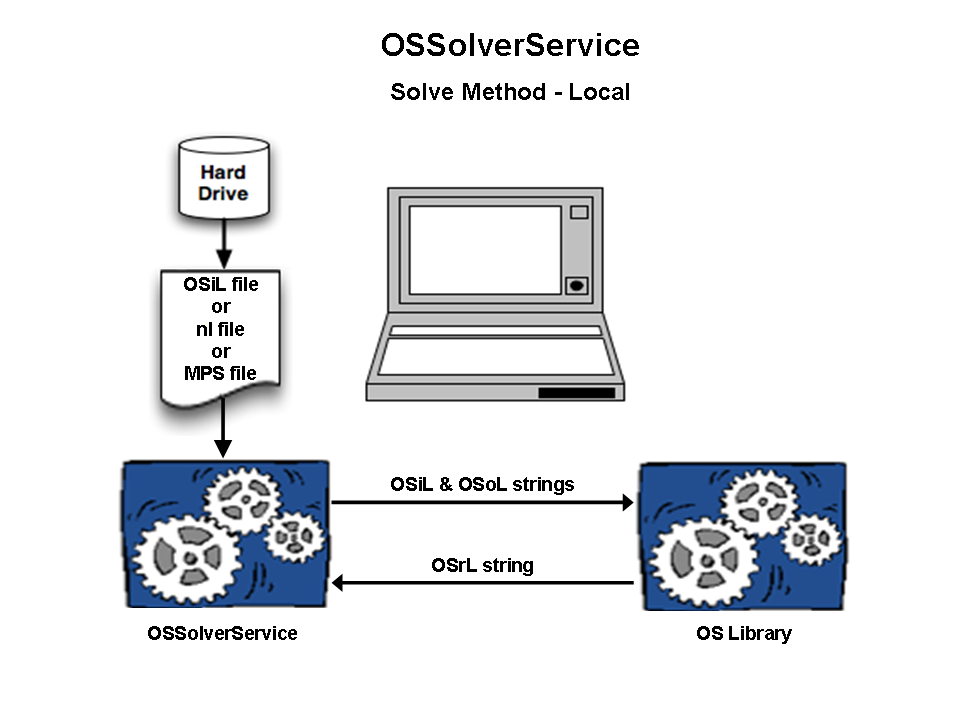
\includegraphics[scale=0.5]{./figures/Figure9.png}
\caption{A local call to {\tt solve}.}
\label{figure:ossolverservicelocal}
\end{figure}



Here is an example of using a configure file,  {\tt testlocal.config}\index{testlocal.config@{\tt testlocal.config}|(},
to invoke {\tt Ipopt}\index{COIN-OR projects!Ipopt@{\tt Ipopt}} locally using the {\tt solve}\index{solve@{\tt solve}} command.

\begin{verbatim}
-osil ../data/osilFiles/parincQuadratic.osil
-solver ipopt
-serviceMethod solve
-browser /Applications/Firefox.app/Contents/MacOS/firefox
-osrl /Users/kmartin/temp/test.osrl
\end{verbatim}



The first line of {\tt testlocal.config}\index{testlocal.config@{\tt testlocal.config}|)} gives the local location
of the OSiL file,
{\tt parincQuadratic.osil}, that contains the problem instance. The second parameter,
{\tt -solver ipopt},  is the solver to be invoked, in this case COIN-OR Ipopt.
The third parameter {\tt -serviceMethod solve} is not really needed, since the default solver service 
is {\tt solve}. It is included only for illustration. 
The fourth parameter is the location of the browser on the local machine. 
The fifth parameter is  {\tt osrl}. The value of this parameter, {\tt /Users/kmartin/temp/test.osrl}, 
specifies the location on the local machine where the OSrL\index{OSrL} result file will get written.


Parameters may also be contained in an XML-file in OSoL\index{OSoL} format. In the configuration file
{\tt testlocalosol.config} we illustrate specifying the instance location in an OSoL file.
\begin{verbatim}
-osol ../data/osolFiles/demo.osol
-solver clp
\end{verbatim}
The file {\tt demo.osol} is

\begin{verbatim}
<?xml version="1.0" encoding="UTF-8"?>
<osol xmlns="os.optimizationservices.org"
      xmlns:xsi="http://www.w3.org/2001/XMLSchema-instance"
      xsi:schemaLocation="os.optimizationservices.org
      http://www.optimizationservices.org/schemas/2.0/OSiL.xsd">
    <general>
        <instanceLocation locationType="local">
            ../data/osilFiles/parincLinear.osil
        </instanceLocation>
    </general>
</osol>
\end{verbatim}


\subsection{Solving Problems Remotely with Web Services}\label{section:servicemethods}

In many cases the client machine may be a ``weak client'' and  using a more powerful machine to solve a
hard optimization instance is required. Indeed, one of the major purposes of Optimization Services is to
facilitate optimization in a distributed environment.   We now provide examples that illustrate using the
{\tt OSSolverService} executable to call a remote solver service.   By remote solver service we mean a
solver service that is called using Web Services.  The OS implementation  of the solver service
uses Apache Tomcat\index{Apache Tomcat}. See \url{tomcat.apache.org}. The Web Service running on the server
is a Java program based on Apache Axis\index{Apache Axis}. See \url{ws.apache.org/axis}. This is described
in greater detail in Section~\ref{section:tomcat}.
This Web Service is called {\tt OSSolverService.jws}\index{OSSolverService.jws@{\tt OSSolverService.jws}}.
It is not necessary to use the Tomcat/Axis combination.



See Figure~\ref{figure:ossolverservice} for an illustration of this process.
The client machine uses {\tt OSSolverService} executable to call one of the
six service methods, e.g., {\tt solve}\index{solve@{\tt solve}}. 
The  information such as the problem
instance in OSiL\index{OSiL} format and solver options in OSoL\index{OSoL} format are packaged into
a SOAP\index{SOAP protocol} envelope and sent to the server. The server is running the Java Web
Service {\tt OSSolverService.jws}. This Java program running in the Tomcat
Java Servlet container implements the six service methods. If a {\tt solve}
or {\tt send} request is sent to the server from the client, an optimization
problem must be solved. The Java solver service solves the optimization instance
by  calling the  {\tt OSSolverService} on the server. So there is an {\tt OSSolverService}
on the client that calls the Web Service {\tt  OSSolverService.jws} that in turn
calls  the executable {\tt OSSolverService} on the server.
The Java solver service passes options to the local {\tt OSSolverService}
%such as where the OSiL file is located and where to write the solution result.
in form of two strings, an osil string representing the instance and an osol string
representing the options (if any). 


For remote calls the instance location can be specified either as a command parameter 
(on the command line or in a config file)
or through the {\tt <instanceLocation>} element in the OSoL\index{OSoL} options file.
OSiL files specified in the {\tt <instanceLocation>} element must be converted to an osil string
by the solver service.
If two instance files
are specified in this way --- one through the local command interface, the other in an options file --- 
the solver service is free to pick which one to choose.





\begin{figure}
\centering
%\includegraphics[scale=0.5]{\figurepath/OSSolverService.png}
%\includegraphics[scale=0.5]{./figures/OSSolverService.png}
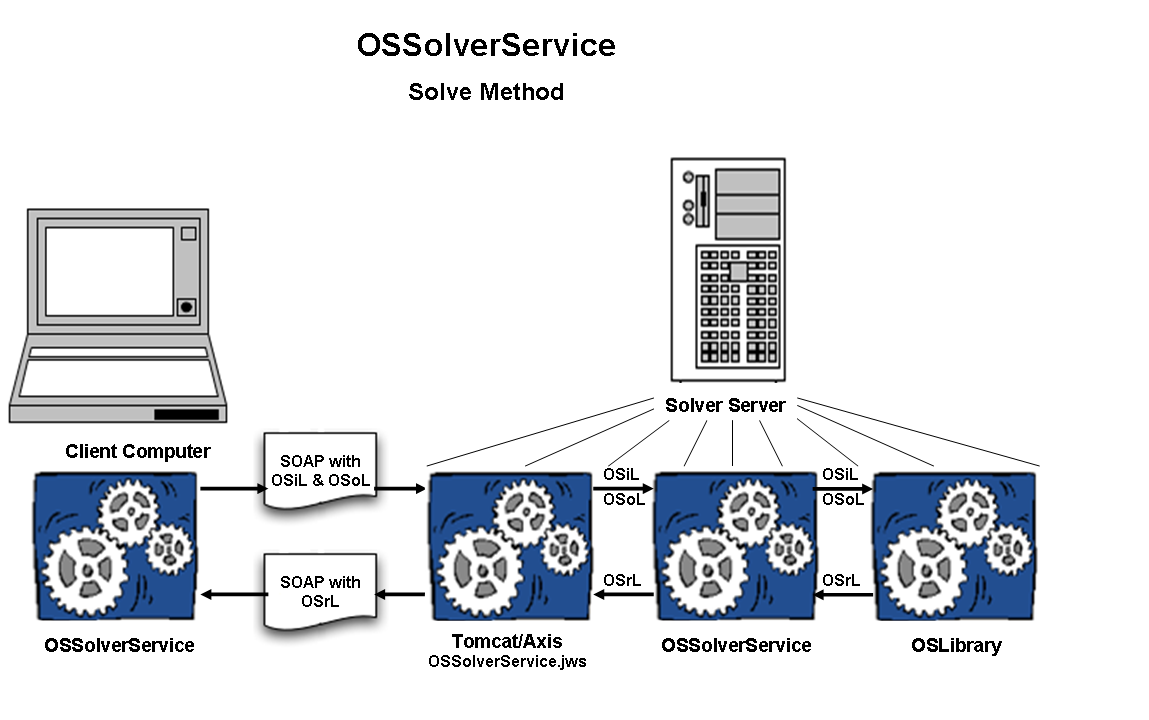
\includegraphics[scale=0.5]{./figures/Figure10.png}
\caption{A remote call to {\tt solve}.}
\label{figure:ossolverservice}
\end{figure}


In the following sections we illustrate each of the six service methods.

\subsubsection{The  {\tt solve} Service Method}\label{section:solve}

\index{solve@{\tt solve}|(}
First we illustrate a simple call to  {\tt OSSolverService.jws}.  The call on the client machine is
\index{testremote.config@{\tt testremote.config}|(}
\begin{verbatim}
./OSSolverService -config ../data/configFiles/testremote.config
\end{verbatim}
where the {\tt testremote.config} file is
\begin{verbatim}
-osil ../data/osilFiles/parincLinear.osil
-serviceLocation http://kipp.chicagobooth.edu/os/OSSolverService.jws
\end{verbatim}

No solver is specified and by default the  {\tt Clp} solver  is used by the {\tt OSSolverService}, 
since the problem is a continuous linar program.
If, for example, the user wished to solve the problem with the {\tt SYMPHONY} solver then this is accomplished
either by using the  {\tt -solver} option on the command line
\begin{verbatim}
./OSSolverService -config ../data/configFiles/testremote.config -solver symphony
\end{verbatim}
or by  adding  the line
\begin{verbatim}
 -solver symphony
\end{verbatim}
to the  {\tt testremote.config} file\index{testremote.config@{\tt testremote.config}|)}.

\index{remoteSolve1.osol@{\tt remoteSolve1.osol}|(}
Next we illustrate a call to the remote SolverService and specify an OSiL instance that is actually residing
on the remote machine that is hosting the {\tt OSSolverService} and not on the client machine.
\begin{verbatim}
./OSSolverService -osol ../data/osolFiles/remoteSolve1.osol
     -serviceLocation  http://kipp.chicagobooth.edu/os/OSSolverService.jws
\end{verbatim}
where the {\tt remoteSolve1.osol} file is
\begin{verbatim}
<?xml version="1.0" encoding="UTF-8"?>
<osol xmlns="os.optimizationservices.org"
      xmlns:xsi="http://www.w3.org/2001/XMLSchema-instance"
      xsi:schemaLocation="os.optimizationservices.org
      http://www.optimizationservices.org/schemas/2.0/OSiL.xsd">
    <general>
        <instanceLocation locationType="local">c:\parincLinear.osil</instanceLocation>
        <contact transportType="smtp">kipp.martin@chicagogsb.edu</contact>
        <solverToInvoke>ipopt</solverToInvoke>      
    </general>
</osol>
\end{verbatim}
\index{remoteSolve1.osol@{\tt remoteSolve1.osol}|)}

If we were to change the {\tt locationType} attribute in the {\tt <instanceLocation>} element to {\tt http} then we
could specify the instance location on yet another machine. This is illustrated below  for {\tt remoteSolve2.osol}.
The scenario is depicted in Figure~\ref{figure:ossolverservice2}.  The OSiL string passed from the client to the solver
service is empty.  However, the OSoL element {\tt <instanceLocation>}  has an attribute {\tt locationType} equal to
{\tt http}.  In this case, the text of the {\tt <instanceLoction>} element contains the URL of a third machine which
has the problem instance {\tt parincLinear.osil}.  The solver service will contact the machine with URL
{\tt\UrlParinclinear} and download this test problem. So the {\tt OSSolverService} is
running on the server {\tt kipp.chicagobooth.edu} which contacts the server {\tt www.coin-or.org} for the model instance.
\begin{verbatim}
<?xml version="1.0" encoding="UTF-8"?>
<osol xmlns="os.optimizationservices.org"
      xmlns:xsi="http://www.w3.org/2001/XMLSchema-instance"
      xsi:schemaLocation="os.optimizationservices.org
      http://www.optimizationservices.org/schemas/2.0/OSiL.xsd">
    <general>
        <instanceLocation locationType="http">
            http://www.coin-or.org/OS/parincLinear.osil
        </instanceLocation>
        <solverToInvoke>ipopt</solverToInvoke>      
    </general>
</osol>
\end{verbatim}

\begin{figure}
\centering
%\includegraphics[scale=0.5]{\figurepath/OSSolverService2.png}
%\includegraphics[scale=0.5]{./figures/OSSolverService2.png}
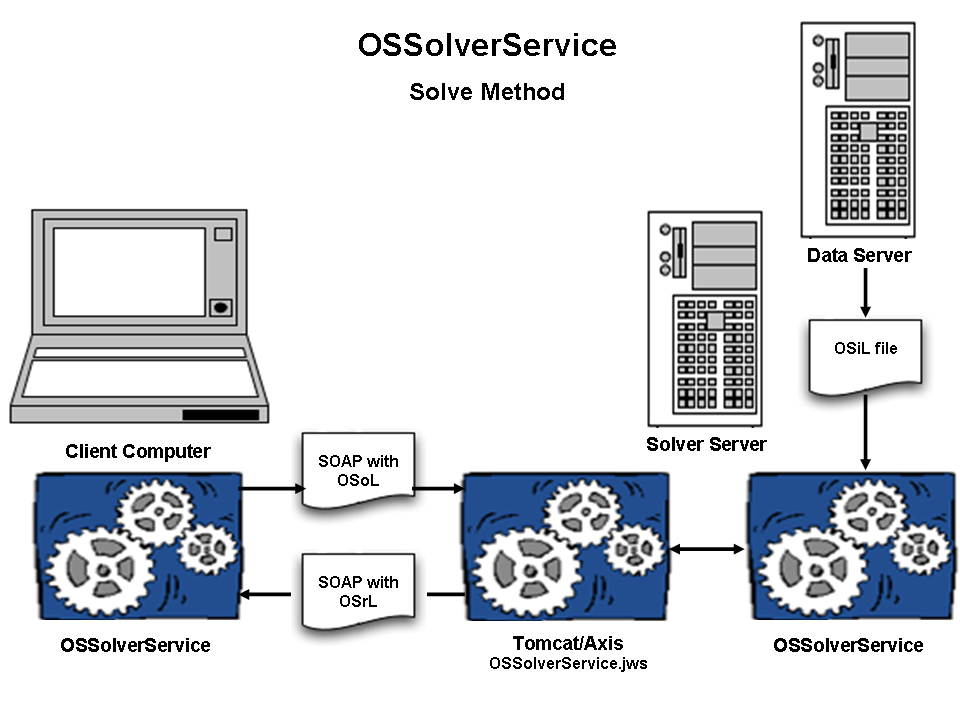
\includegraphics[scale=0.5]{./figures/Figure11.png}
\caption{Downloading the instance from a remote source.}
\label{figure:ossolverservice2}
\end{figure}

{\bf Note:} The {\tt solve} method communicates synchronously with the remote solver service
and once started, these jobs cannot be killed. This may not be desirable for large
problems when the user does not want to wait for a response or when there is a possibility
for the solver to enter an infinite loop. The {\tt send} service
method should be used when asynchronous communication is desired.\index{solve@{\tt solve}|)}


\subsubsection{The  {\tt send} Service Method}\label{section:send}

\index{send@{\tt send}|(}
When the {\tt solve} service method is used, then the {\tt OSSolverService} does not
finish execution until the solution is returned from the remote solver service.
 When the {\tt send}
method is used, the instance is communicated to the remote service and the
{\tt OSSolverService} terminates after submission. An example of this is
\begin{verbatim}
./OSSolverService -config ../data/configFiles/testremoteSend.config
\end{verbatim}
where the {\tt testremoteSend.config} file is
\begin{verbatim}
-nl ../data/amplFiles/hs71.nl
-serviceLocation http://kipp.chicagobooth.edu/os/OSSolverService.jws
-serviceMethod send
\end{verbatim}
In this example the COIN-OR {\tt Ipopt}\index{COIN-OR projects!Ipopt@{\tt Ipopt}} solver is specified. The input file {\tt hs71.nl}
is in AMPL nl format\index{AMPL nl format|(}.
Before sending this to the remote solver service the {\tt OSSolverService} executable converts  
the nl format\index{AMPL nl format|)} into the OSiL\index{OSiL} XML format and packages this 
into the SOAP\index{SOAP protocol} envelope used by Web Services.

Since the {\tt send} method involves asynchronous communication the remote solver service must keep track of jobs.
The {\tt send} method requires a {\tt JobID}\index{JobID@{\tt JobID}|(}. In the above example no {\tt JobID} was specified.
When no {\tt JobID} is specified the {\tt OSSolverService} method first invokes the {\tt getJobID} service method
to get a {\tt JobID}, puts this information into an OSoL\index{OSoL|(} file it creates, and sends the information
to the server. More information on the {\tt getJobID} service method is provided in Section~\ref{section:getjobid}.
The {\tt OSSolverService} prints the OSoL file to standard output before termination.
This is illustrated below,

\begin{verbatim}
<?xml version="1.0" encoding="UTF-8"?>
<osol xmlns="os.optimizationservices.org"
      xmlns:xsi="http://www.w3.org/2001/XMLSchema-instance"
      xsi:schemaLocation="os.optimizationservices.org
      http://www.optimizationservices.org/schemas/2.0/OSiL.xsd">
    <general>
        <jobID>
            gsbrkm4__127.0.0.1__2007-06-16T15.46.46.075-05.00149771253
        </jobID>
        <solverToInvoke>ipopt</solverToInvoke>      
    </general>
</osol>
\end{verbatim}

The {\tt JobID} is one that is randomly generated by the server and passed back to the {\tt OSSolverService}.
The user can also provide a {\tt JobID} in their OSoL file. For example, below is a user-provided OSoL file that could
be specified in a configuration file or on the command line.

\begin{verbatim}
<?xml version="1.0" encoding="UTF-8"?>
<osol xmlns="os.optimizationservices.org"
      xmlns:xsi="http://www.w3.org/2001/XMLSchema-instance"
      xsi:schemaLocation="os.optimizationservices.org
      http://www.optimizationservices.org/schemas/2.0/OSiL.xsd">
    <general>
        <jobID>123456abcd</jobID>
        <solverToInvoke>ipopt</solverToInvoke>      
    </general>
</osol>
\end{verbatim}

The same {\tt JobID} cannot be used twice, so if {\tt 123456abcd} was used earlier, the result of {\tt send} will be
{\tt false}\index{JobID@{\tt JobID}|)}.

In order to be of any use, it is necessary to get the result of the optimization. This is described in
Section~\ref{section:retrieve}. Before proceeding to this section, we describe two ways for knowing when
the optimization is complete. One feature of the standard OS remote SolverService is the ability to send an
email when the job is complete. Below is an example of the {\tt OSoL} that uses the email feature\index{OSoL|)}.

\begin{verbatim}
<?xml version="1.0" encoding="UTF-8"?>
<osol xmlns="os.optimizationservices.org"
      xmlns:xsi="http://www.w3.org/2001/XMLSchema-instance"
      xsi:schemaLocation="os.optimizationservices.org
      http://www.optimizationservices.org/schemas/2.0/OSiL.xsd">
    <general>
        <jobID>123456abcd</jobID>
        <contact transportType="smtp">
            kipp.martin@chicagogsb.edu
        </contact>
        <solverToInvoke>ipopt</solverToInvoke>      
    </general>
</osol>
\end{verbatim}

The remote Solver Service will send an email to the above address when the job is complete. A second option for
knowing when a job is complete is to use the {\tt knock}\index{knock@{\tt knock}} method.
(See Section~\ref{section:knock}.)

Note that in all of these examples we provided a value for the {\tt <solverToInvoke>} element.
%The remote solver service will use {\tt Cbc} if another solver is not specified.%
A default solver is used (see Table~\ref{table:defaultsolvers}\index{default solver} if another solver is not specified.%
\index{send@{\tt send}|)}



\subsubsection{The  {\tt retrieve} Service Method}\label{section:retrieve}

\index{retrieve@{\tt retrieve}|(}
The {\tt retrieve} method is used to get information about the instance solution.  This method has a single string argument which is an OSoL instance. Here is an example of using the {\tt retrieve} method with {\tt OSSolverService}.
\begin{verbatim}
./OSSolverService -config ../data/configFiles/testremoteRetrieve.config
\end{verbatim}
The {\tt testremoteRetrieve.config} file is
\begin{verbatim}
-serviceLocation http://kipp.chicagobooth.edu/os/OSSolverService.jws
-osol ../data/osolFiles/retrieve.osol
-serviceMethod retrieve
-osrl /home/kmartin/temp/test.osrl
\end{verbatim}
and the {\tt retrieve.osol} file is

\begin{verbatim}
<?xml version="1.0" encoding="UTF-8"?>
<osol xmlns="os.optimizationservices.org"
      xmlns:xsi="http://www.w3.org/2001/XMLSchema-instance"
      xsi:schemaLocation="os.optimizationservices.org
      http://www.optimizationservices.org/schemas/2.0/OSiL.xsd">
    <general>
        <jobID>123456abcd</jobID>
    </general>
</osol>
\end{verbatim}

The OSoL file {\tt retrieve.osol} contains a tag {\tt <jobID>} that is communicated to
the remote service. The remote service locates the result and returns it as a string.
The {\tt <jobID>}\index{JobID@{\tt JobID}} should reflect a {\tt <jobID>} that was previously submitted
using a {\tt send()} command.
The result is returned as a string in OSrL format.  The user must modify the line
\begin{verbatim}
-osrl /home/kmartin/temp/test.osrl
\end{verbatim}
to reflect a valid path for their own machine.  (It is also possible to delete the line
in which case the result will be displayed on the screen instead of being saved to the
file indicated in the {\tt -osrl} option.)\index{retrieve@{\tt retrieve}|)}


\subsubsection{The  {\tt getJobID} Service Method}\label{section:getjobid}

\index{getJobID@{\tt getJobID}|(}
Before  submitting a job with the {\tt send}\index{send@{\tt send}} method a {\tt JobID}\index{JobID@{\tt JobID}}
is required. The {\tt OSSolverService} can get a {\tt JobID} with the following options.
\begin{verbatim}
-serviceLocation http://kipp.chicagobooth.edu/os/OSSolverService.jws
-serviceMethod getJobID
\end{verbatim}
Note that no OSoL\index{OSoL} input file is specified. In this case, the {\tt OSSolverService} sends an empty string.
A string is returned with the {\tt JobID}. This {\tt JobID} is then put into a {\tt <jobID>} element in an
OSoL string that would be used by the {\tt send}\index{send@{\tt send}} method.
\index{getJobID@{\tt getJobID}|)}


\subsubsection{The  {\tt knock} Service Method}\label{section:knock}

\index{knock@{\tt knock}|(}
The OSSolverService terminates after executing the {\tt send}\index{send@{\tt send}} method. Therefore,
it is necessary to know when the job is completed on the remote server. One way is to include an email
address in the  {\tt <contact>}  element with the attribute {\tt transportType} set to {\tt smtp}.
This was illustrated in Section~\ref{section:solve}.  A second way to check on the status of a job is
to use the {\tt knock} service method.  For example, assume a user   wants to know if  the job
with {\tt JobID 123456abcd}\index{JobID@{\tt JobID}}  is complete. A user would make the request
\begin{verbatim}
./OSSolverService -config ../data/configFiles/testRemoteKnock.config
\end{verbatim}
where the {\tt testRemoteKnock.config} file is
\begin{verbatim}
-serviceLocation http://kipp.chicagobooth.edu/os/OSSolverService.jws
-osplInput ../data/osolFiles/demo.ospl
-osol ../data/osolFiles/retrieve.osol
-serviceMethod knock
\end{verbatim}
the {\tt demo.ospl} file is

% header to be temporarily hidden...
% <ospl xmlns="os.optimizationservices.org">
%       xmlns:xsi="http://www.w3.org/2001/XMLSchema-instance"
%       xsi:schemaLocation="os.optimizationservices.org
%       http://www.optimizationservices.org/schemas/2.0/OSiL.xsd">

\begin{verbatim}
<?xml version="1.0" encoding="UTF-8"?>
<ospl xmlns="os.optimizationservices.org">
    <processHeader>
        <request action="getAll"/>
    </processHeader>
    <processData/>
</ospl>
\end{verbatim}
and the {\tt retrieve.osol} file is
\begin{verbatim}
<?xml version="1.0" encoding="UTF-8"?>
<osol xmlns="os.optimizationservices.org"
      xmlns:xsi="http://www.w3.org/2001/XMLSchema-instance"
      xsi:schemaLocation="os.optimizationservices.org
      http://www.optimizationservices.org/schemas/2.0/OSiL.xsd">
    <general>
        <jobID>123456abcd</jobID>
    </general>
</osol>
\end{verbatim}

The result of this request is a string in OSpL\index{OSpL|(} format, with the data contained in its
{\tt processData} section.  The result is displayed on the screen; if the user desires it
to be redirected to a file, a command should be added to the {\tt testRemoteKnock.config}
file with a valid path name on the local system, e.g.,

\begin{verbatim}
-osplOutput ./result.ospl
\end{verbatim}

Part of the return format is illustrated below.

% Header to be temporarily hidden
% <ospl xmlns="os.optimizationservices.org"
%       xmlns:xsi="http://www.w3.org/2001/XMLSchema-instance"
%       xsi:schemaLocation="os.optimizationservices.org
%       http://www.optimizationservices.org/schemas/2.0/OSiL.xsd">

\begin{verbatim}
<?xml version="1.0" encoding="UTF-8"?>
<ospl xmlns="os.optimizationservices.org">
  <processHeader>
    <serviceURI>http://localhost:8080/os/ossolver/CGSolverService.jws</serviceURI>
    <serviceName>CGSolverService</serviceName>
    <time>2006-05-10T15:49:26.7509413-05:00</time>
  <processHeader>
  <processData>
     <statistics>
        <currentState>idle</currentState>
        <availableDiskSpace>23440343040</availableDiskSpace>
        <availableMemory>70128</availableMemory>
        <currentJobCount>0</currentJobCount>
        <totalJobsSoFar>1</totalJobsSoFar>
        <timeServiceStarted>2006-05-10T10:49:24.9700000-05:00</timeServiceStarted>
        <serviceUtilization>0.1</serviceUtilization>
        <jobs>
        <job jobID="123456abcd">
            <state>finished</state>
            <serviceURI>http://kipp.chicagobooth.edu/ipopt/IPOPTSolverService.jws</serviceURI>
            <submitTime>2007-06-16T14:57:36.678-05:00</submitTime>
            <startTime>2007-06-16T14:57:36.678-05:00</startTime>
            <endTime>2007-06-16T14:57:39.404-05:00</endTime>
            <duration>2.726</duration>
          </job>
        </jobs>
     </statistics>
  </processData>
</ospl>
\end{verbatim}
Notice that the {\tt <state>} element in {\tt <job jobID="123456abcd">} indicates that the job is finished.

When making a {\tt knock} request,  the OSoL string can be empty. In this example, if the OSoL string had been empty
the status of all jobs kept in the file ospl.xml is reported.  In our default solver service implementation,
there is a configuration file {\tt OSParameter} that has a parameter {\tt MAX\_JOBIDS\_TO\_KEEP }.
The current default setting is~100. In a large-scale or commercial implementation it might be wise to keep
problem results and statistics in a database. Also, there are values other than {\tt getAll} (i.e., get all
process information related to the jobs) for the OSpL {\tt action} attribute in the {\tt <request>} tag.
For example, the {\tt action} can be set to a value of {\tt ping} if the user just wants
to check if the remote solver service is up and running. For details, check the OSpL schema.\index{OSpL|)}
\index{knock@{\tt knock}|)}


\subsubsection{The  {\tt kill}   Service Method}

\index{kill@{\tt kill}|(}
If the user submits a job that is taking too long or is a mistake, it is possible to kill the job on the remote server using the {\tt kill} service method.
For example, to kill job {\tt 123456abcd}, at the command line type
\begin{verbatim}
./OSSolverService -config  ../data/configFiles/kill.config
\end{verbatim}
where the configure file {\tt kill.config} is
\begin{verbatim}
-osol ../data/osolFiles/kill.osol
-serviceLocation http://kipp.chicagobooth.edu/os/OSSolverService.jws
-serviceMethod kill
\end{verbatim}
and the {\tt kill.osol} file is
\begin{verbatim}
<?xml version="1.0" encoding="UTF-8"?>
<osol xmlns="os.optimizationservices.org"
      xmlns:xsi="http://www.w3.org/2001/XMLSchema-instance"
      xsi:schemaLocation="os.optimizationservices.org
      http://www.optimizationservices.org/schemas/2.0/OSiL.xsd">
    <general>
        <jobID>123456abcd</jobID>
    </general>
</osol>
\end{verbatim}

The result is returned in  OSpL format.
\index{kill@{\tt kill}|)}



\subsubsection{Summary and description of the API}

The six service methods just described are also available as callable routines.
Below is a summary of the inputs and outputs of the six methods. See also Figure~\ref{figure:osCommunicationMethods}.
A test program illustrating the use of the methods is described in Section~\ref{section:exampleOSRemoteTest}.

\begin{itemize}

\item {\tt solve( osil, osol ):}\index{solve@{\tt solve}}

\begin{itemize}

\item Inputs: a string with the instance in OSiL\index{OSiL} format and an optional string with the solver options
in OSoL\index{OSoL} format

\item Returns: a string with the solver solution in OSrL\index{OSrL} format

\item Synchronous call, blocking request/response

\end{itemize}



\item {\tt send( osil, osol ):}\index{solve@{\tt solve}}

\begin{itemize}

\item Inputs: a string with the instance in OSiL\index{OSiL} format and a string with the solver options
in OSoL\index{OSoL} format (same as in {\tt solve})

\item Returns:  a boolean, true if the problem was successfully submitted, false otherwise

\item Has the same signature as {\tt solve}

\item Asynchronous (server side), non-blocking call

\item The {\tt osol} string should have a {\tt JobID}\index{JobID@{\tt JobID}} in the {\tt <jobID>} element
\end{itemize}


\item {\tt getJobID( osol ):}\index{getJobID@{\tt getJobID}}

\begin{itemize}

\item Inputs: a string  with the solver options in OSoL\index{OSoL} format (in this case, the string
may be empty because no options are required to get the JobID)

\item Returns: a string which is the unique job id generated by the solver service

\item Used to maintain session and state on a distributed system
\end{itemize}



\item {\tt knock( ospl, osol ):}\index{knock@{\tt knock}}

\begin{itemize}

\item Inputs: a string in OSpL\index{OSpL} format and an optional string with the solver options in OSoL\index{OSoL} format

\item Returns: process and job status information from the remote server in OSpL format

\end{itemize}


\item {\tt retrieve( osol ):}\index{retrieve@{\tt retrieve}}

\begin{itemize}

\item Inputs: a string with the solver options  in OSoL\index{OSoL} format

\item Returns: a string with the solver solution in OSrL\index{OSrL} format

\item The {\tt osol} string should have a {\tt JobID}\index{JobID@{\tt JobID}} in the {\tt <jobID>} element

\end{itemize}


\item {\tt kill( osol ):}\index{kill@{\tt kill}}

\begin{itemize}

\item Inputs: a string with the solver options  in OSoL\index{OSoL} format

\item Returns: process and job status information from the remote server in OSpL\index{OSpL} format

\item Critical in long running optimization jobs

\end{itemize}

\end{itemize}
\index{OSSolverService@{\tt OSSolverService}|)}


\begin{figure}[ht]
\centering
%\includegraphics[scale=0.5]{\figurepath/osCommunicationMethods.pdf}
\includegraphics[scale=0.5]{./figures/osCommunicationMethods.pdf}
\caption{The OS Communication Methods}
\label{figure:osCommunicationMethods}
\end{figure}


\subsection{Passing Options to Solvers}

The OSoL (Optimization Services option Language) protocol is used to pass options to solvers.   
When using the {\tt OSSolverService} executable this will typically be done through an OSoL XML file 
by specifying the {\tt -osol} option followed by the location of the file.  However, it is also possible 
to write a custom application that links to the OS library and to build an OSOption object in memory 
and then pass this to a solver. We next describe the  feature of the OSoL protocol that will be the most 
useful to the typical user.

In the OSoL protocol there is an element {\tt <solverOptions>} that can have any number of {\tt <solverOption>} 
children. (See the file {\tt parsertest.osol} in OS/data/osolFiles.)  Each {\tt <solverOption>} child can have 
six attributes, all of which except one are optional. These attributes are:

\begin{itemize}

\item {\bf name:} this is the only required attribute and is the option name. It should be unique.

\item {\bf value:}  the value of the option.

\item {\bf solver:} the name of the solver associated with the option.

\item {\bf type:} this will usually be a data type (such as integer, string, double, etc.) but this is not necessary.

\item {\bf category:} the same solver option may apply to multiple categories so it may be necessary to specify a 
category for solver. For example, in LINDO an option can apply to a specific model or to every model in an environment. 
Hence we might have

\begin{verbatim}
<solverOption name="LS_IPARAM_LP_PRINTLEVEL" 
   solver="lindo" category="model"  type="integer" value="0"/>
<solverOption name="LS_IPARAM_LP_PRINTLEVEL" 
   solver="lindo" category="environment" type="integer" value="1"/>
\end{verbatim}
where we specify the print level for a specific model or the entire environment.   The category attribute should be 
separated by a colon (`:') if there is more than one  category or  additional subcategories, 
as in the following hypothetical example.
\begin{verbatim}
<solverOption name="hypothetical" 
   solver="SOLVER" category="cat1:subcat2:subsubcat3" 
      type="string" value="illustration"/>
\end{verbatim}

\item {\bf description:} a description of the option; typically this would not get passed to the solver.

\end{itemize}

As of trunk version 2164\index{OS project!trunk version} the reading of an
OSoL file is implemented in the {\tt OSCoinSolver}, {\tt OSBonmin} and
{\tt OSIpopt} solver interfaces.   The  {\tt OSBonmin}, and {\tt OSIpopt}
solvers have particularly easy interfaces. They have methods for integer,
string, and numeric data types and then take options in form of
{\tt (name, value)} pairs. Below is an example of options for {\tt Ipopt}.


\begin{verbatim}
<solverOption name="mu_strategy" solver="ipopt" 
     type="string" value="adaptive"/>
<solverOption name="tol" solver="ipopt" 
     type="numeric" value="1.e-9"/>
<solverOption name="print_level" solver="ipopt" 
     type="integer" value="5"/>
<solverOption name="max_iter" solver="ipopt" 
     type="integer" value="2000"/>
\end{verbatim}

We have also implemented the {\tt OSOption} class for the {\tt OSCoinSolver} interface. This can be done in two ways. 
First, options can be set through the Osi Solver interface (the OSCoinSolver interface wraps around the Osi Solver interface).    
We have implemented all of the options listed in {\tt OsiSolverParameters.hpp} in {\tt Osi} trunk version 1316.  
In the Osi solver interface, in addition to string, double, and integer types  there is a type called {\tt HintParam}
and a type called {\tt OsiHintParam}. The value of the {\tt OsiHintParam} is an {\tt OsiHintStrength} type, 
which may be confusing. For example, to have the following Osi method called

\begin{verbatim}
setHintParam(OsiDoReducePrint, true, hintStrength);
\end{verbatim}


the user should set the following {\tt <solverOption>} tags:
\begin{verbatim}
<solverOption name="OsiDoReducePrint" solver="osi" 
    type="OsiHintParam"  value="true" />
<solverOption name="OsiHintIgnore" solver="osi" 
     type="OsiHintStrength" />
\end{verbatim}
There should be only one {\tt <solverOption>} with type {\tt OsiHintStrength} and if there are more than one in the 
OSoL file (string) the last one is the one implemented. 

In addition to setting options using the Osi  Solver interface, it is possible to pass options directly to the {\tt Cbc} 
solver. By default the following options are sent to the {\tt Cbc} solver,

\begin{verbatim}
-log=0  -solve 
\end{verbatim}
The option {\tt -log=0} will keep the branch-and-bound output to a minimum.  Default options are overridden by 
putting into the OSoL file at least one {\tt <solverOption>} tag with the {\tt solver} attribute 
set to {\tt cbc}.    For example, the following sequence of options will limit the search to 100 nodes, 
cut generation turned off.

\begin{verbatim}
<solverOption name="maxN" solver="cbc" value="100" />
<solverOption name="cuts" solver="cbc" value="off" />
<solverOption name="solve" solver="cbc"  />
\end{verbatim}

Any option that {\tt Cbc} accepts at the command line can be put into a {\tt <solverOption>} tag. We list  those below.

{\small
\begin{verbatim}
Double parameters:
  dualB(ound)  dualT(olerance)  primalT(olerance)  primalW(eight)  
Branch and Cut double parameters:
  allow(ableGap)  cuto(ff)  inc(rement)  inf(easibilityWeight)  integerT(olerance)  
  preT(olerance)  ratio(Gap)  sec(onds)  
Integer parameters:
  cpp(Generate)  force(Solution)  idiot(Crash)  maxF(actor)  maxIt(erations)  
  output(Format)  slog(Level)  sprint(Crash)  
Branch and Cut integer parameters:
  cutD(epth)  log(Level)  maxN(odes)  maxS(olutions)  passC(uts)  
  passF(easibilityPump)  passT(reeCuts)  pumpT(une)  strat(egy)  strong(Branching)  
  trust(PseudoCosts)  
Keyword parameters:
  chol(esky)  crash  cross(over)  direction  dualP(ivot)  
  error(sAllowed)  keepN(ames)  mess(ages)  perturb(ation)  presolve  
  primalP(ivot)  printi(ngOptions)  scal(ing)  
Branch and Cut keyword parameters:
  clique(Cuts)  combine(Solutions)  cost(Strategy)  cuts(OnOff)  Dins  
  DivingS(ome)  DivingC(oefficient)  DivingF(ractional)  DivingG(uided)  DivingL(ineSearch)  
  DivingP(seudoCost)  DivingV(ectorLength)  feas(ibilityPump)  flow(CoverCuts)  gomory(Cuts)  
  greedy(Heuristic)  heur(isticsOnOff)  knapsack(Cuts)  lift(AndProjectCuts)  local(TreeSearch)  
  mixed(IntegerRoundingCuts)  node(Strategy)  pivot(AndFix)  preprocess  probing(Cuts)  
  rand(omizedRounding)  reduce(AndSplitCuts)  residual(CapacityCuts)  Rens  Rins  
  round(ingHeuristic)  sos(Options)  two(MirCuts)  
Actions or string parameters:
  allS(lack)  barr(ier)  basisI(n)  basisO(ut)  directory  
  dirSample  dirNetlib  dirMiplib  dualS(implex)  either(Simplex)  
  end  exit  export  help  import  
  initialS(olve)  max(imize)  min(imize)  netlib  netlibD(ual)  
  netlibP(rimal)  netlibT(une)  primalS(implex)  printM(ask)  quit  
  restore(Model)  saveM(odel)  saveS(olution)  solu(tion)  stat(istics)  
  stop  unitTest  userClp  
Branch and Cut actions:
  branch(AndCut)  doH(euristic)  miplib  prio(rityIn)  solv(e)  
  strengthen  userCbc  
\end{verbatim}
}


The user may also wish to specify an initial starting solution. This is particularly
useful with interior point methods.  This is accomplished by using the
{\tt <initialVariableValues>} tag.  Below we illustrate how to set the
initial values for variables with an index of 0, 1, and~3.

\begin{verbatim}
<initialVariableValues numberOfVar="3">
   <var idx="0" value="1"/>
   <var idx="1" value="4.742999643577776" />
   <var idx="3" value="1.379408293215363"/>
</initialVariableValues>
\end{verbatim}

As of trunk version 2164\index{OS project!trunk version} the initial values for variables can be passed
to the {\tt Bonmin} and {\tt Ipopt} solvers.


When implementing solver options in-memory, the typical calling sequence is:

\begin{verbatim}
solver->buildSolverInstance();
solver->setSolverOptions();
solver->solve();
\end{verbatim}






\section{Setting up a Solver Service with Apache Tomcat}\label{section:tomcat}

\index{Apache Tomcat|(}
This section explains how to download and use the Java implementation of the
remote solver service described in Section~\ref{section:servicemethods}.
The server side of the Java distribution is based on the Tomcat~6.0
implementation. In order to build an OS Solver Service, the user should do an
svn checkout:

\begin{verbatim}
svn co https://projects.coin-or.org/svn/OS/branches/OSjava OSjava
\end{verbatim}

The {\tt OSjava} folder contains the file {\tt INSTALL.txt}. Please follow the
instructions in {\tt  INSTALL.txt} under the heading:
\begin{verbatim}
== Install An OS Web Server==
\end{verbatim}

Installing the OS Web Server based on the instructions in {\tt INSTALL.txt}
assumes that the user has installed:

\begin{itemize}
  \item Eclipse IDE.  See  \url{http://www.eclipse.org/downloads/}. At this
  link we recommend that the user get {\tt Eclipse Classic}.  
  
  \item An {\tt OSSolverService} that is compatible  with the server platform.  
  The {\tt OSSolverService} executable for several different platforms is
  available at \url{http://www.coin-or.org/download/binary/OS/OSSolverService/}. 
  The user can also build the executable as described in this Manual.  See
  Section \ref{section:build}.
  
  \item Tomcat 6.0. See \url{http://tomcat.apache.org/}.
\end{itemize}

After the final installation is complete on the server we recommend testing  by
doing someting like the following. On a client machine, create  the file {\tt
testremote.config} with the following lines of text
\begin{verbatim}
-serviceLocation http://***.***.***.***:8080/OSServer/services/OSSolverService
-osil /parincLinear.osil
\end{verbatim}
where {\tt ***.***.***.***} is the IP address of the Tomcat server machine. Then, assuming the files
{\tt testremote.config} and {\tt parincLinear.osil} are in the same directory on the client machine as the
{\tt OSSolverService} execute:
\begin{verbatim}
./OSSolverService -config testremote.config
\end{verbatim}
You should get back an OSrL result printed to the screen.




\vskip 8pt
In the following discussion, we assume that the root folder for Tomcat running
on the server is named {\tt tomcat}. \vskip 8pt

If you already have a Tomcat 6.0 server with Axis installed, and have created an
{\tt OSServer.war} file based on {\tt INSTALL.txt}, do the following:
\begin{enumerate}
\item{} copy the file {\tt OSServer.war} into the Tomcat {\tt tomcat/webapps}
directory.

\item{}  Stop and start Tomcat.
\end{enumerate}

In the directory,
\begin{verbatim}
tomcat/webapps/OSServer/WEB-INF/code/OSConfig
\end{verbatim}
there is a configuration file {\tt OSParameter.xml} that can be modified to fit individual user needs. 
You can configure such parameters as service name, service URL/URI. 
Refer to the xml file for more detail. Descriptions for all the parameters are within the file itself.

\vskip 8pt

Below is a summary of the common and important directories
 and files you may want to know.

\begin{itemize}
\item
\begin{verbatim}
tomcat/webapps/OSServer/
\end{verbatim}
contains the OS Solver Service Web application. All directories and files
outside of this folder are Tomcat server related.
\item
\begin{verbatim}
tomcat/webapps/OSServer/WEB-INF
\end{verbatim}
contains private and important configuration, library, class and executable files to run the Optimization Service.

\item
\begin{verbatim}
tomcat/webapps/OSServer/WEB-INF/code/OSConfig
\end{verbatim}
contains configuration files for Optimization Services, such as the {\tt OSParameter.xml} file.
\item
\begin{verbatim}
tomcat/webapps/OSServer/WEB-INF/code/temp
\end{verbatim}
contains temporarily saved files such as submitted OSiL/OSoL input files, and OSrL output files. This folder can get bigger as the service starts to run more jobs. For maintenance purpose, you may want to keep an eye on it.
\item
\begin{verbatim}
tomcat/webapps/OSServer/WEB-INF/code/log
\end{verbatim}
contains log files from the running services in the current Web application.
\item
\begin{verbatim}
tomcat/webapps/OSServer/WEB-INF/classes
\end{verbatim}
contains solver binaries that actually carry out the optimization process.
\item
\begin{verbatim}
tomcat/webapps/OSServer/WEB-INF/code/backup
\end{verbatim}
contains backup files from some of the above directories. This folder can get bigger as the service starts to run more jobs.
\item
\begin{verbatim}
tomcat/webapps/OSServer/WEB-INF/classes
\end{verbatim}
contains class files to run the Optimization Services.
\item
\begin{verbatim}
tomcat/webapps/OSServer/WEB-INF/lib
\end{verbatim}
contains library files needed by the Optimization Services.
\item
\begin{verbatim}
tomcat/conf
\end{verbatim}
contains configuration files for the Tomcat server, such as http server port.
\item
\begin{verbatim}
tomcat/bin
\end{verbatim}
contains executables and scripts to start and shut down the Tomcat server.
\end{itemize}
\index{Apache Tomcat|)}



\section{OS Support for Modeling Languages, Spreadsheets and Numerical Computing Software}\label{section:modellang}

Algebraic modeling languages can be used to generate model instances as input to an OS compliant solver.
We describe two such hook-ups, {\tt OSAmplClient} for AMPL\index{AMPL}, and {\tt CoinOS} for GAMS\index{GAMS} (version 23.3 and above).


\subsection{AMPL Client:  Hooking AMPL to Solvers}\label{section:amplclient}

\index{OSAmplClient@{\tt OSAmplClient}|(}
\index{AMPL|(}




%This section is based on the assumption that the user has installed  AMPL  on his or her machine.   
It is possible to call all of the COIN-OR solvers listed in %Section~\ref{section:overview} 
Table~\ref{table:configurations}~(p.\pageref{table:configurations})
directly from the  AMPL (see {\tt http://www.ampl.com}) modeling language.  In this discussion we assume 
the user has already obtained and installed AMPL.  
Both the binary download described in Section~\ref{section:obtainingbinaries}
and the unix and Windows builds (Section \ref{section:unixbuilds}
and~\ref{section:windowsinstall}, respectively) contain
%In  the download described in Section~\ref{section:binary} there is 
an executable, {\tt OSAmplClient.exe},
that is linked to all of the COIN-OR solvers  listed in Table~\ref{table:configurations}. %Section~\ref{section:overview}.   
From the  perspective of AMPL, the   {\tt OSAmplClient} acts like an AMPL ``solver''.    
The {\tt OSAmplClient.exe}   can be used to solve problems either locally or remotely.   


\subsubsection{Using OSAmplClient for a Local Solver}\label{section:localampl}

In the following discussion we assume that the AMPL executable {\tt ampl.exe}, the {\tt OSAmplClient},  
and the test problem {\tt  eastborne.mod}\index{eastborne.mod@{\tt eastborne.mod}|(}
 are all in the same directory.  

The  problem instance {\tt eastborne.mod} is an AMPL model file included in the OS distribution 
in the {\tt amplFiles}\index{amplFiles@{\tt amplFiles}} directory.  To solve this problem locally 
by calling {\tt OSAmplClient.exe} from AMPL, first start AMPL and then open the {\tt eastborne.mod} file 
inside AMPL.  The test model {\tt eastborne.mod} is a linear integer program. 

\begin{verbatim}
# take in sample integer linear problem
# assume the problem is in the AMPL directory
model eastborne.mod;
\end{verbatim}

The next step is to tell AMPL that the solver it is going to use is {\tt OSAmplClient.exe}. 
Do this by issuing the following command inside AMPL.

\begin{verbatim}
# tell AMPL that the solver is OSAmplClient
option solver OSAmplClient;
\end{verbatim}

It is not necessary to provide the  {\tt OSAmplclient.exe} solver with any options. 
You can just issue the {\tt solve} command in AMPL as illustrated below.  

\begin{verbatim}
# solve the problem
solve;
\end{verbatim}

Of the six methods described in Section~\ref{section:ossolverservice} only the {\tt solve} method 
has been implemented to date.

If no options are specified, the default solver is used, depending on the problem characteristics 
(see Table~\ref{table:defaultsolvers}).\index{default solver}
%is to use {\tt Clp}\index{Clp@{\tt Clp}} for linear programs. 
%For continuous nonlinear models {\tt Ipopt}\index{Ipopt@{\tt Ipopt}} is used. 
%For mixed-integer linear models, {\tt Cbc}\index{Cbc@{\tt Cbc}} is used. 
%For mixed-integer nonlinear models  {\tt Bonmin}\index{Bonmin@{\tt Bonmin}} is used.  
If you wish to specify a specific solver, use the {\tt -solver} option.   For example,  
since the test problem {\tt eastborne.mod} is a linear integer program, {\tt Cbc} is used by default. 
If you want to instead use {\tt SYMPHONY}\index{COIN-OR projects!SYMPHONY@{\tt SYMPHONY}|(},
then you would pass a {\tt solver} option to the {\tt OSAmplclient.exe} solver as follows.%
\index{eastborne.mod@{\tt eastborne.mod}|)}

\begin{verbatim}
# now tell OSAmplClient to use SYMPHONY instead of Cbc
option OSAmplClient_options "-solver symphony";
\end{verbatim}

Valid values for the {\tt -solver} option are {\tt bonmin}, {\tt cbc}, {\tt clp}, {\tt couenne}, 
{\tt dylp}, {\tt symphony}, and {\tt vol}.   The solver name in the {\tt -solver} option is case insensitive.  


\subsubsection{Using OSAmplClient to Invoke the COIN-OR Solver Server}\label{section:remoteampl}

Next, assume that you have a large problem you want to solve on the remote solver. It is necessary 
to specify the location of the server solver as an option to OSAmplClient. 
The {\tt -serviceLocation} option is used to specify the location of a solver server. 
In this case, the string of options for {\tt OSAmplClient\_options} is:

\begin{verbatim}
-serviceLocation  http://webdss.ise.ufl.edu:2646/OSServer/services/OSSolverService
\end{verbatim}

This string is used to replace the string `{\tt -solver symphony}' in the previous example. 
We will omit the other parts (i.e., the AMPL instruction
\begin{verbatim}
option OSAmplClient_options
\end{verbatim}
the double quotes and the trailing semicolon) in this and the remaining examples.
 
This option will send the problem to the solver server at location {\tt http://webdss.ise.ufl.edu}.   


\medskip


Each call 
\begin{verbatim}
option OSAmplClient_options
\end{verbatim}
is memoryless. That is, the options set in the last call will overwrite any options set in previous calls
and cause them to be discarded.

For instance, the sequence of option calls
\begin{verbatim}
option OSAmplClient_options "-solver symphony";
option OSAmplClient_options "-serviceLocation  
    http://webdss.ise.ufl.edu:2646/OSServer/services/OSSolverService";
solve;
\end{verbatim}
will result in the default solver being called. 

\medskip

Finally, the user may wish to pass options to the individual solver. This is done by providing an options file.
A sample options file, {\tt solveroptions.osol}\index{solveroptions.osol@{\tt solveroptions.osol}} is 
provided with this distribution.  The name of the options file is the value of the {\tt -osol} option.
The string of options to {\tt OSAmplClient\_options} is now
\begin{verbatim}
-serviceLocation http://webdss.ise.ufl.edu:2646/OSServer/services/OSSolverService
-osol solveroptions.osol
\end{verbatim}
This   {\tt solveroptions.osol}  file contains four solver options; two for {\tt Cbc}, one for {\tt Ipopt}, 
and one for {\tt SYMPHONY}\index{COIN-OR projects!SYMPHONY@{\tt SYMPHONY}|)}.
You can have any number of options. Note the format for specifying an option:
\begin{verbatim}
<solverOption name="maxN" solver="cbc" value="5" />
\end{verbatim}
The attribute {\tt name} specifies that the option name is {\tt maxN} which is the maximum number of nodes 
allowed in the branch-and-bound tree, the {\tt solver} attribute specifies the name of the solver that the 
option should be applied to, and the {\tt value} attribute specifies the value of the option. 
As a second example, consider the specification
\begin{verbatim}
<solverOption name="max_iter" solver="ipopt" type="integer" value="2000"/> 
\end{verbatim}
In this example we are specifying an iteration limit for {\tt Ipopt}.  Note the additional attribute 
{\tt type} that has value  {\tt integer}. The Ipopt solver requires specifying the data type 
(string, integer, or numeric) for its options.   Different solvers have different options, 
and we recommend that the user look at the documentation for the solver of interest in order to see 
which options are available.  
A good summary of options for COIN-OR solvers is \url{http://www.coin-or.org/GAMSlinks/gamscoin.pdf}.


If you examine the file {\tt solveroptions.osol} you will see that there is an XML tag  with the name
{\tt <solverToInvoke>} and that the solver given is {\tt symphony}.   
This has no effect on a local solve. However, if this option file is paired with 

\begin{verbatim}
-serviceLocation http://webdss.ise.ufl.edu:2646/OSServer/services/OSSolverService
-osol solveroptions.osol
\end{verbatim}
then in our reference implementation the remote solver service will parse the file {\tt solveroptions.osol}, find the {\tt <solverToInvoke>} tag and then pass the {\tt symphony} solver option to the {\tt OSSolverService} on the remote server.

\subsubsection{AMPL Summary}

\begin{enumerate}
\item Tell  AMPL to use the OSAmplClient as the solver:

\begin{verbatim}
option solver OSAmplClient;
\end{verbatim}

\item Specify options to the OSAmplclient solver by using the AMPL command {\tt OSAmplClient\_options}.

\item There are three possible options to specify:

\begin{itemize}

\item the name of the solver using the  {\tt -solver} option; valid values for this option  are {\tt clp}, 
{\tt cbc},  {\tt dylp},  {\tt ipopt}, {\tt bonmin},   {\tt couenne},  {\tt symphony}, and {\tt vol};


\item the location of the remote server using   the {\tt -serviceLocation} option;

\item the location of the options file using  the {\tt -osol} option.

\end{itemize}

These three options behave {\it exactly like} the {\tt -solver}, {\tt -serviceLocation}, and {\tt -osol} options used by the {\tt OSSolverService} described in  Section \ref{section:commandlineparser}.


\item If no options are specified using {\tt OSAmplClient\_options},  the default solver is used.
(For details see Table~\ref{table:defaultsolvers}).\index{default solver}
%
% by default, for continuous
%inear models  {\tt clp} is used. For continuous nonlinear models {\tt ipopt} is used. 
%For mixed-integer linear models (MIP),   {\tt cbc} is used. For mixed-integer nonlinear models  
%\tt bonmin} is used.  
%
All solvers are invoked locally. 

\item  The options given to {\tt OSAmplClient\_options}  can be given in any order.

\item A remote solver is called if and only if the {\tt -serviceLocation} option is specified.

\end{enumerate}

\index{OSAmplClient@{\tt OSAmplClient}|)}
\index{AMPL|)}



\subsection{GAMS and Optimization Services}\label{section:gamslinks}

\index{GAMS|(}

This section pertains to GAMS version 23.3 (and above) that now includes support for OS.  
Here we describe the GAMS  implementation of Optimization Services.  We assume that the user has installed GAMS.

There are two ways to access an OS Solver Service from GAMS, on the local machine or on a remote server.
The difference between the two approaches is explained in the next two sections.

\subsubsection{Using GAMS to Invoke the Local OS Solver Service \tt CoinOS}\label{section:gamslocal}

   
In GAMS,  OS is implemented through the {\tt CoinOS} solver that is packaged with GAMS.      
The GAMS {\tt CoinOS} solver is really a {\it solver interface} and is linked through the OS library to the 
following COIN-OR solvers: {\tt Bonmin}, {\tt Cbc}, {\tt Clp},  {\tt Glpk}, and {\tt Ipopt}. 
Think of {\tt CoinOS} as a {\it metasolver}.    As an example (we assume a Windows operating system 
and use the .exe extension), consider:

\begin{verbatim}
gams.exe eastborne.gms MIP=CoinOS
\end{verbatim}
The solver name {\tt CoinOS} is not case sensitive and 
\begin{verbatim}
gams.exe eastborne.gms MIP=coinos
\end{verbatim}
will also work.  In addition, if
\begin{verbatim}
Option MIP = CoinOS ;
\end{verbatim}
is present in the GAMS file, then writing {\tt MIP=CoinOS} on the command line is unnecessary.
Since {\tt Option MIP = CoinOS;} is present in the GAMS model file {\tt eastborne.gms}, 
we will not specify it explicitly on the command line in the ensuing discussion. To summarize,
\begin{verbatim}
gams.exe eastborne.gms 
\end{verbatim}
is equivalent to the two versions of the command given previously.  Executing any of the commands will 
result in the model being solved on the local machine using the COIN-OR solver {\tt Cbc}, the default solver 
for 
%continuous linear models (LP and RMIP), {\tt CoinOS} chooses {\tt Clp}. For continuous nonlinear 
%models (NLP, DNLP, RMINLP, QCP, RMIQCP), {\tt Ipopt} is the default solver. For 
mixed-integer linear models (MIP).
%,  {\tt Cbc} is the default solver. For mixed-integer nonlinear models (MIQCP, MINLP), 
%{\tt Bonmin} is the default solver.

It is possible to control which solver is selected by {\tt CoinOS}.    This is done by providing an {\it options file}  to  GAMS.   
Since the solver is named {\tt  CoinOS}, the options file should  be named {\tt CoinOS.opt}  (the file name is not case sensitive)
and the command line call is 
\begin{verbatim}
gams.exe eastborne.gms optfile 1
\end{verbatim}
Calling multiple GAMS options files uses the convention
\begin{verbatim}
optfile=1 corresponds to CoinOS.opt
optfile=2 corresponds to CoinOS.op2
...
optfile=99 corresponds to CoinOS.o99
\end{verbatim}

We now explain the valid options that can go into a GAMS option file when using the {\tt CoinOS} solver.  They are:

\vskip 8pt
\noindent {\tt solver  (string)}:   Specifies the solver that is used to solve an instance. 
Valid values are {\tt clp},  {\tt cbc}, {\tt glpk}, {\tt ipopt},  and {\tt bonmin}.  
If a solver name is specified that is not recognized, the default solver for the problem type is used.  
The value for the solver option is case insensitive. 
For example, if the file {\tt CoinOS.opt} contains a single line
\begin{verbatim}
solver glpk
\end{verbatim}
then executing
\begin{verbatim}
gams.exe eastborne.gms optfile 1
\end{verbatim}
will result in  using {\tt Glpk}  to solve the problem.   


\vskip 8pt
\noindent {\tt writeosil  (string)}:  If this option is used, GAMS will write the optimization instance 
to file {\tt (string)} in    OSiL   format.
\vskip 8pt

\vskip 8pt
\noindent {\tt writeosrl  (string)}:  If this option is used, GAMS will write the result of the optimization 
to file {\tt (string)} in OSrL  format.
\vskip 8pt

The options just described are options for the GAMS modeling language.  
It is also possible to pass options directly to the COIN-OR solvers by using the {\tt OS} interface.
This is done by passing the name of an options file that conforms to the  OSoL  standard.  
%See \url{http://projects.coin-or.org/OS}  for information on Optimization Services.  
The option

\vskip 8pt
\noindent {\tt readosol  (string)}  specifies the name of an OS option  file in OSoL format that is 
given to the solver.  Note: The file  {\tt CoinOS.opt} is an option  file for GAMS but the GAMS option 
{\tt readosol} in the GAMS options file  is specifying the name of an OS options file. 
\vskip 8pt
The file {\tt solveroptions.osol} is contained in the OS distribution in the {\tt osolFiles} directory   
in the {\tt data} directory. This file contains four solver options; two for {\tt Cbc}, one for {\tt Ipopt},
and one for {\tt SYMPHONY} (which is available for remote server calls, but not locally).  
You can have any number of options. Note the format for specifying an option:
\begin{verbatim}
<solverOption name="maxN" solver="cbc" value="5" />
\end{verbatim}
The attribute {\tt name} specifies that the option name is {\tt maxN} which is the maximum number of nodes 
allowed in the branch-and-bound tree, the {\tt solver} attribute specifies the name of the solver to which
the option should be applied, and the {\tt value} attribute specifies the value of the option. 

As a second example, consider the specification
\begin{verbatim}
<solverOption name="max_iter" solver="ipopt" type="integer" value="2000"/> 
\end{verbatim}
In this example we are specifying an iteration limit for {\tt Ipopt}.  Note the additional attribute 
{\tt type} that has value  {\tt integer}. The Ipopt solver requires specifying the data type 
(string, integer, or numeric) for its options.   For a list of options that solvers take, 
see the file
\begin{verbatim}
docs/solvers/coin.pdf
\end{verbatim}
inside the GAMS directory. 
An up-to-date online version of this list is available at \url{http://www.coin-or.org/GAMSlinks/gamscoin.pdf}.



\subsubsection{Using GAMS  to Invoke a Remote OS Solver Service}\label{section:gamsremote}

We now describe how to call  a remote OS   solver service using the GAMS {\tt CoinOS}.  Before proceeding, 
it is important to emphasize that when calling a remote OS solver service, the remote service may be a 
different implementation of OS than the GAMS implementation in {\tt CoinOS}. For example, the remote 
implementation may also provide access to solvers such as {\tt SYMPHONY}, {\tt Couenne}, and {\tt DyLP}.  
There are several reason why you might wish to use a remote OS solver service. 

\begin{itemize}
\item Have access to a faster machine.

\item  Be able to  submit jobs to run in asynchronous mode -- submit your job,  turn off your laptop,  
and check later to see if the job ran.

\item Call several additional solvers ({\tt SYMPHONY}, {\tt Couenne} and {\tt DyLP}).

\end{itemize}

In order to use  the COIN-OR solver service it is necessary to specify the service URL. 
This is done using the {\tt service} option.

\vskip 8pt
\noindent{\tt service (string)}: Specifes the URL of  the COIN-OR solver service
\vskip 8pt
Use the following value for this option.
\begin{verbatim}
service http://webdss.ise.ufl.edu:2646/OSServer/services/OSSolverService
\end{verbatim}

%For linear models (LP and RMIP),  {\tt Clp} is the default solver. For continuous nonlinear models 
%(NLP, DNLP, RMINLP, QCP, RMIQCP), {\tt Ipopt} is the default solver. For mixed-integer linear models (MIP),
%{\tt  Cbc} is the default solver. For mixed-integer nonlinear models (MIQCP, MINLP), {\tt Bonmin} is 
%the default solver.  
Default solver values are present, depending on the problem for characteristics. For more details, consult 
Table~\ref{table:defaultsolvers} (p.\pageref{table:defaultsolvers}).
In order to control the solver used, it is necessary to specify the name of the solver
inside the XML tag {\tt <solverToInvoke>}. The example  {\tt solveroptions.osol} file contains the XML tag
\begin{verbatim}
<solverToInvoke>symphony</solverToInvoke>
\end{verbatim}
If, for example,  the {\tt CoinOS.opt} file is
\begin{verbatim}
solver ipopt
service http://webdss.ise.ufl.edu:2646/OSServer/services/OSSolverService
readosol  solveroptions.osol
writeosrl temp.osrl
\end{verbatim}
then {\tt Ipopt} is ignored as a solver option and the remote server uses the {\tt  SYMPHONY} solver.  
Valid values for the remote solver service specified in the {\tt <solverToInvoke>} tag are {\tt clp},  
{\tt cbc},  {\tt dylp}, {\tt glpk}, {\tt ipopt}, {\tt bonmin},   {\tt couenne},  {\tt symphony}, and 
{\tt vol}.  If the problem is solved using a remote solver service the value specified by the GAMS {\tt solver} option is irrelevant and ignored. 

The GAMS {\tt CoinOS} solver behaves differently from other implementiations of OS
%the {\tt OSAmplClient} 
in the following way.  
Although it is  possible to put the address of the remote server in the OS options file, it is not read 
by the GAMS {\tt CoinOS} solver. The only way to specify a remote solver is through the GAMS  
{\tt service} option.



By default, the call to the server is a {\it synchronous} call. The GAMS process will wait for the result 
and then display the result. This may not be desirable when solving large optimization models.  
The user may wish to submit a job, turn off his or her computer,  and then check at a later date to see 
if the job is finished.  In order to use the remote solver service in this fashion, i.e., 
{\it asynchronously}, it  is necessary to use the  {\tt service\_method} option.

\vskip 8pt
\noindent {\tt service\_method (string)} specifies the method to execute on a server.  
Valid values for this option are {\tt solve}, {\tt getJobID}, {\tt send}, {\tt knock}, {\tt retrieve}, 
and {\tt kill}. We explain how to use each of these.
\vskip 8pt
The default value of {\tt service\_method} is {\tt solve.} A {\tt solve} invokes the remote service 
in synchronous mode. When using the {\tt solve} method you can optionally specify a set of solver options 
in an OSoL file  by using the {\tt readosol} option. The  remaining values for the {\tt service\_method} 
option are used for an asynchronous call.  We illustrate them in the order in which they would most 
logically be executed. 

\vskip 8pt
\noindent {\tt service\_method getJobID}: When working in asynchronous mode, the server needs to 
uniquely identify each job. The {\tt getJobID} service method will result in the server returning 
a unique job id. For example if the following {\tt CoinOS.opt} file is used
\vskip 8pt
\begin{verbatim}
service http://webdss.ise.ufl.edu:2646/OSServer/services/OSSolverService
service_method getJobID
\end{verbatim}
with the command
\begin{verbatim}
gams.exe eastborne.gms optfile=1
\end{verbatim}
the user will see a rather long job id returned to the screen as output. Assume that the job id returned 
is {\tt coinor12345xyz}. This job id is used to submit a job to the server with the {\tt send} method.
Any job id can be sent to the server as long as it has not been used before.  

\vskip 8pt
\noindent {\tt service\_method send}: When working in asynchronous mode, use the {\tt send} service method 
to submit a job. When using  the {\tt send} service method option an option is required and the options file
must specify a  job id that has not been used before.  Assume that in the  {\tt CoinOS.opt}  we specify 
the options:
\vskip 8pt
\begin{verbatim}
service http://webdss.ise.ufl.edu:2646/OSServer/services/OSSolverService
service_method send
readosol sendWithJobID.osol
\end{verbatim}
The {\tt sendWithJobID.osol} options file is identical to the {\tt solveroptions.osol} options file except 
that it has an additional XML tag:
\begin{verbatim}
<jobID>coinor12345xyz</jobID> 
\end{verbatim}
We then execute
\vskip 8pt
\begin{verbatim}
gams.exe eastborne.gms optfile=1
\end{verbatim}
If all goes well, the response to the above command should  be: ``Problem instance successfully sent to 
OS service''. At this point the server will schedule the job and work on it. It is possible to turn off 
the user computer at this point. At some point the user will want to know if the job is finished. 
This is accomplished using the {\tt knock} service method.
\vskip 8pt
\noindent {\tt service\_method knock}: When working in asynchronous mode, this is used to check the status 
of a job.  Consider the following {\tt CoinOS.opt} file:
\vskip 8pt
\begin{verbatim}
service http://webdss.ise.ufl.edu:2646/OSServer/services/OSSolverService
service_method knock
readosol sendWithJobID.osol 
readospl knock.ospl
writeospl knockResult.ospl
\end{verbatim}
The {\tt knock} service method requires two  inputs. The first input is the name of an options file, 
in this case {\tt sendWithJobID.osol}, specified through the {\tt readosol} option. In addition, a file 
in OSpL format is required. You can use the {\tt knock.opsl} file provided in the binary distribution. 
This file name is specified using the {\tt readospl} option. If no job id is specified in the OSoL file 
then the status of all jobs on the server will be returned in the file specified by the {\tt writeospl} 
option. If a job id is specified in the OSoL file, then only information on the specified job id is 
returned in the file specified by the {\tt writeospl} option.  In this case the file name is 
{\tt knockResult.ospl}. We then execute
\vskip 8pt
\begin{verbatim}
gams.exe eastborne.gms optfile=1
\end{verbatim}
The file {\tt knockResult.ospl} will contain the information
\begin{verbatim}
<job jobID="coinor12345xyz">
<state>finished</state>
<serviceURI>http://192.168.0.219:8443/os/OSSolverService.jws</serviceURI>
<submitTime>2009-11-10T02:13:11.245-06:00</submitTime>
<startTime>2009-11-10T02:13:11.245-06:00</startTime>
<endTime>2009-11-10T02:13:12.605-06:00</endTime>
<duration>1.36</duration>
 </job>
\end{verbatim}
Note that the job is complete as indicated in the {\tt <state>} tag. It is now time to actually retrieve 
the job solution.  This is done with the {\tt retrieve} method.
\vskip 8pt
\noindent {\tt service\_method retrieve}: When working in asynchronous mode, this method is used 
to retrieve the job solution. It is necessary when using {\tt retrieve} %{\tt knock} ???
to specify an options file and in that options file specify a job id.   
Consider the following {\tt CoinOS.opt} file:
\vskip 8pt
\begin{verbatim}
service http://webdss.ise.ufl.edu:2646/OSServer/services/OSSolverService
service_method retrieve
readosol sendWithJobID.osol
writeosrl answer.osrl
\end{verbatim}
When we then execute
\vskip 8pt
\begin{verbatim}
gams.exe eastborne.gms optfile=1
\end{verbatim}
the result is written to the file {\tt answer.osrl}. 

Finally there is a {\tt kill} service method which is used to kill a job that was submitted by mistake 
or is running too long on the server. 
\vskip 8pt
\noindent {\tt service\_method kill:} When working in asynchronous mode, this method is used to terminate 
a job. You should specify an OSoL  file containing the JobID by using the {\tt readosol} option.
\vskip 8pt


\subsubsection{GAMS Summary:}\label{section:gamssummary}


\begin{enumerate}

\item[1.]   In order to use OS with GAMS you can either specify {\tt CoinOS} as an option to GAMS 
at the command line,
\begin{verbatim}
gams eastborne.gms MIP=CoinOS
\end{verbatim}
or you can  place the statement {\tt Option ProblemType = CoinOS;} somewhere in the model {\it before} 
the {\tt Solve} statement in the GAMS file.


\item[2.]   If no options are given, then the model will be solved locally using the default solver 
(see Table~\ref{table:defaultsolvers} on p.\pageref{table:defaultsolvers}).
%and {\tt Clp} will be used for 
%linear programs, {\tt Cbc} for integer linear programs, {\tt Ipopt} for continuous nonlinear programs, 
%and {\tt Bonmin} for nonlinear integer programs.

\item[3.] In order to control behavior (for example, whether a local or remote solver is used)  an options
 file,  {\tt CoinOS.opt}, must be used as follows

\begin{verbatim}
gams.exe  eastborne.gms optfile=1
\end{verbatim}

\item[4.]  The  {\tt CoinOS.opt} file is used to specify {\it eight potential options}:


\begin{itemize}
\item {\tt service (string)}: using the COIN-OR solver server; this is done by giving the option

\begin{verbatim}
service  http://webdss.ise.ufl.edu:2646/OSServer/services/OSSolverService
\end{verbatim}


\item  {\tt readosol (string)}: whether or not to send the solver an options file; this is done by 
giving the option
\begin{verbatim}
readosol  solveroptions.osol
\end{verbatim}


\item   {\tt solver (string)}: if a local solve is being done,  a specific solver is specified by 
the option
\begin{verbatim}
solver solver_name
\end{verbatim}

Valid values are {\tt clp},  {\tt cbc}, {\tt glpk}, {\tt ipopt} and {\tt bonmin}. %  and {\tt couenne}.  
When the COIN-OR solver service is being used, the only way to specify the solver to use is through 
the {\tt <solverToInvoke>} tag in an OSoL file. In this case the valid values for the solver are  
{\tt clp}, {\tt cbc}, {\tt dylp}, {\tt glpk}, {\tt ipopt}, {\tt bonmin}, {\tt couenne}, {\tt symphony}
and {\tt vol}.



\item  {\tt writeosrl (string)}:  the solution result can be put into an OSrL file by specifying the option

\begin{verbatim}
writeosrl  osrl_file_name
\end{verbatim}



\item    {\tt writeosil (string)}:   the optimization instance  can be put into an OSiL file by specifying 
the option



\begin{verbatim}
writeosil  osil_file_name
\end{verbatim}


\item {\tt writeospl (string):} Specifies the name of an OSpL  file in which the answer from the 
{\tt knock} or {\tt kill} method is written, e.g.,

\begin{verbatim}
writeospl  write_ospl_file_name
\end{verbatim}


\item {\tt readospl (string):} Specifies the name of an OSpL  file that the {\tt knock} method 
sends to  the server

\begin{verbatim}
readospl  read_ospl_file_name
\end{verbatim}

\item {\tt service\_method (string)}: Specifies the method to execute on a server.  Valid values 
for this option are {\tt solve}, {\tt getJobID}, {\tt send}, {\tt knock}, {\tt retrieve}, and {\tt kill}.

\end{itemize}

\item[5.]  If an OS options file is passed to the GAMS {\tt CoinOS} solver using the GAMS  {\tt CoinOS} option      {\tt readosol}, then GAMS does not interpret  or act on any options in this file. The options in the OS options file are passed directly to either: i) the default local solver, ii) the local solver specified by the  GAMS {\tt CoinOS}  option {\tt solver}, or iii)  to the remote OS solver service if one is specified by the GAMS  {\tt CoinOS} option {\tt service.}

\end{enumerate}

\index{GAMS|)}



\subsection{MATLAB:  Using MATLAB to Build and Run OSiL Model Instances}\label{section:usingmatlab}

\index{MATLAB|(}
This example differs from the other examples in that makefiles are not used.
Indeed, if the user has done a VPATH\index{VPATH} build, the relevant {\tt cpp} file remains
in the original OS download directory under {\tt OS/examples/matlab},
not in the VPATH directory.




Linear, integer, and quadratic problems can be formulated in MATLAB and then optimized
either locally or over the network using the OS Library. The {\tt OSMatlab} class functions much like
{\tt OSnl2osil}\index{OSnl2osil@{\tt OSnl2osil}} and {\tt OSmps2osil}\index{OSmps2osil@{\tt OSmps2osil}}
and takes MATLAB arrays to create an OSiL instance.  This class is part of the OS library.
In order to use the {\tt OSMatlab} class it is necessary to  compile
{\tt OSmatlabSolver.cpp}  into  a MATLAB Executable ({\tt mex}) file.
The {\tt OSmatlabSolver.cpp} file is in the {\tt  OS/examples/matlab} directory.
We  assume the user has already done a {\tt make install} and that in the OS root directory
\begin{verbatim}
/Users/kmartin/Documents/files/code/cpp/OScpp/COIN-OS
\end{verbatim}
there is an {\tt include} directory as well as a {\tt lib} directory resulting from the {\tt make install}.
The following steps should be followed.


\begin{enumerate}[{\bf Step 1:}]



\item{} Edit the MATLAB file {\tt mexopts.sh} (UNIX) or {\tt mexopts.bat}  (Windows) so that the {\tt CXXFLAGS} option includes the header files in the {\tt cppad} directory and the {\tt include} directory in the project root. For example, it  should look like:
\begin{verbatim}
CXXFLAGS='-fno-common -no-cpp-precomp -fexceptions
    -I/Users/kmartin/Documents/files/code/cpp/OScpp/COIN-OS/
    -I/Users/kmartin/Documents/files/code/cpp/OScpp/COIN-OS/include'
\end{verbatim}

Next edit the {\tt CXXLIBS} flag so that the OS and supporting libraries are included. For example, it should look like:

\begin{verbatim}
CXXLIBS="$MLIBS -lstdc++
    -L/Users/kmartin/Documents/files/code/ipopt/macosx/Ipopt-3.2.2/lib
    -L/Users/kmartin/Documents/files/code/cpp/OScpp/COIN-OSX/lib
    -lOS  -lbonmin -lIpopt -lOsiCbc -lOsiClp -lOsiSym -lCbc -lCgl -lOsi -lClp
    -lSym -lCoinUtils  -lm"
\end{verbatim}

For a UNIX system the {\tt mexopts.sh} file  is typically  found in a directory with the release name in 
{\tt  $\sim$/.matlab}. For example, {\tt $\sim$/.matlab/R14SP3}.  It may also be in the {\tt bin} directory 
in the MATLAB application root folder.


On a Windows system, the {\tt  mexopts.bat} file will usually be in a directory with the release name in 
{\tt C:$\backslash$Documents and Settings$\backslash$Username$\backslash$Application Data$\backslash$Mathworks$\backslash$MATLAB}


\item{}  Build the MATLAB executable file. Start MATLAB and in the MATLAB command window connect to the directory {\tt OS/examples/matlab} which  contains the file {\tt OSmatlabSolver.cpp}.    Execute the command:

\begin{verbatim}
mex -v OSMatlabSolver.cpp
\end{verbatim}

On an Intel MAC OS X the resulting executable will be named {\tt OSmatlabSolver.mexmaci}. On the Windows system the file is named {\tt OSmatlabSolver.mexw32}.

\item{}  Set the MATLAB path to include the directory with the {\tt OSmatlabSolver} executable.


\item{}   In the MATLAB command window, connect to the directory {\tt OS/data/matlabFiles}. Run either of the MATLAB
files {\tt markowitz.m} or {\tt parincLinear.m}.  The result should be displayed in the MATLAB browser window.

\end{enumerate}


To use the {\tt OSmatlabSolver} it is necessary to put the coefficients  from a linear, integer, or quadratic problem into MATLAB arrays.   We illustrate for the linear program:

\begin{alignat}{2}
& \mbox{Minimize} & \quad
10 x_{1} + 9 x_{2}\label{eq:parinobj}\\
& \mbox{Subject to} & \quad .7x_{1} + x_{2}  &\le 630  \label{eq:parinccon1}\\
& & .5x_{1} + (5/6) x_{2} &\le 600 \label{eq:parinccon2}\\
& &  x_{1} + (2/3) x_{2} &\le 708 \label{eq:parinccon3}\\
& & .1x_{1} + .25 x_{2} &\le 135 \label{eq:parinccon4}\\
& & x_{1}, x_{2} &\ge 0 \label{eq:parincnonneg}
\end{alignat}

The MATLAB representation of this problem in MATLAB arrays is
\begin{verbatim}
% the number of constraints
numCon = 4;
% the number of variables
numVar = 2;
% variable types
VarType='CC';
% constraint types
A = [.7  1; .5  5/6; 1   2/3  ; .1   .25];
BU = [630 600  708  135];
BL = [];
OBJ = [10  9];
VL = [-inf -inf];
VU = [];
ObjType = 1;
% leave Q empty if there are no quadratic terms
Q = [];
prob_name = 'ParInc Example'
password = 'chicagoesmuyFRIO';
%
%
%the solver
solverName = 'lindo';
%the remote service address
%if left empty we solve locally
serviceAddress='http://kipp.chicagobooth.edu/os/OSSolverService.jws';
% now solve
callMatlabSolver( numVar, numCon, A, BL, BU, OBJ, VL, VU, ObjType, ...
    VarType, Q, prob_name, password, solverName, serviceAddress)
\end{verbatim}
This example m-file is in the {\tt data} directory and is file {\tt parincLinear.m}. Note that in addition to the problem formulation
we can specify which solver to use through the {\tt solverName} variable.  If solution with a remote solver is desired
this can be specified with the {\tt serviceAddress} variable.  If the {\tt serviceAddress} is left empty, i.e.,
\begin{verbatim}
serviceAddress='';
\end{verbatim}
then a local solver is used. In this case  it is crucial that the appropriate solver is linked in with the {\tt matlabSolver}
executable using the {\tt CXXLIBS} option.


The data directory  also contains the m-file  {\tt template.m} which contains extensive comments about how to formulate
the problems in MATLAB.   The user can edit {\tt template.m} as necessary and create a new instance.




 A second example which is a quadratic problem is given in Section~\ref{section:usingmatlab}.
The appropriate MATLAB m-file is {\tt markowitz.m} in the {data/matlabFiles} directory.
The problem consists in investing  in a number of stocks. The expected returns and risks
(covariances) of the stocks are known. Assume that the decision variables $x_i$
represent the fraction of wealth invested in stock~$i$ and that no stock can have
more than 75\% of the total wealth. The problem then is to minimize the total risk
subject to a budget constraint and a lower bound on the expected portfolio return.

Assume that there are three stocks (variables) and two constraints (not counting the upper limit  %investment
of .75 on the investment variables).


\begin{verbatim}
% the number of constraints
numCon = 2;
% the number of variables
numVar = 3;
\end{verbatim}



All the variables are continuous:


\begin{verbatim}
VarType='CCC';
\end{verbatim}


Next define the constraint upper and lower bounds. There are two constraints, an equality  constraint (an $=$) and a lower bound on portfolio return of .15 (a $\ge$). These two constraints are expressed as



\begin{verbatim}
BL = [1   .15];
BU = [1  inf];
\end{verbatim}



The variables are nonnegative and have upper limits of .75 (no stock can comprise more than 75\% of the portfolio).  This is written as




\begin{verbatim}
VL = [];
VU = [.75 .75 .75];
\end{verbatim}



There are no nonzero linear coefficients in the objective function, but the objective function vector must always be defined and the number of components of this vector is the number of variables.



\begin{verbatim}
OBJ = [0 0 0 ]
\end{verbatim}


 Now the linear constraints.   In the model the two linear constraints are
 \begin{eqnarray*}
 x_{1} + x_{2} + x_{3} &=& 1 \\
 0.3221 x_{1} +   0.0963x_{2} +    0.1187x_{3}  &\ge& .15
 \end{eqnarray*}



 These are expressed as



 \begin{verbatim}
 A = [ 1 1 1  ;
  0.3221   0.0963   0.1187 ];
 \end{verbatim}


Now for the quadratic terms. The only quadratic terms are in the objective function. The objective function is


\begin{eqnarray*}
\min  0.425349694 x_{1}^{2} +  0.445784443 x_{2}^{2} + 0.231430983 x_{3}^{2} + 2 \times 0.185218694 x_{1} x_{2} \\
+ 2 \times 0.139312545 x_{1} x_{3} + 2 \times 0.13881692 x_{2} x_{3}
\end{eqnarray*}


The quadratic matrix $Q$ has four rows and a column for each quadratic term. In this example there are six quadratic terms.  
The first row of $Q$ is the row index where the terms appear. By convention, the objective function has index -1 and we count constraints starting at 0.  The first row of $Q$ is


 \begin{verbatim}
 -1 -1 -1 -1 -1 -1
 \end{verbatim}

The second row of $Q$ is the index of the first variable in the quadratic term. We use zero based counting.  Variable $x_{1}$ has index 0, variable  $x_{2}$ has index 1, and variable $x_{3}$ has index 2.  Therefore, the second row of $Q$ is



\begin{verbatim}
0 1 2 0 0 1
\end{verbatim}



The third row of $Q$ is the index of the second variable in the quadratic term.   Therefore, the third row of $Q$ is



\begin{verbatim}
0 1 2  1 2 2
\end{verbatim}



The last (fourth) row is the coefficient. Therefore, the fourth row reads





\begin{verbatim}
.425349654  .445784443  .231430983
.370437388  .27862509   .27763384
\end{verbatim}


The quadratic matrix is



\begin{verbatim}
Q = [ -1 -1 -1 -1 -1 -1;
      0 1 2 0 0 1 ;
      0 1 2 1 2 2;
      .425349654  .445784443  .231430983   ...
      .370437388  .27862509   .27763384
    ];
\end{verbatim}


Finally, name the problem, specify the solver (in this case {\tt ipopt}), the service address (and password if required by the service), and call the solver.



\begin{verbatim}
% replace Template with the name of your  problem
prob_name = 'Markowitz Example from Anderson, Sweeney, Williams, and Martin';
password = 'chicagoesmuyFRIO';
%
%the solver
solverName = 'ipopt';
%the remote service service address
%if left empty we solve locally
serviceAddress='http://kipp.chicagobooth.edu/os/OSSolverService.jws';
% now solve
OSCallMatlabSolver( numVar, numCon, A, BL, BU, OBJ, VL, VU, ObjType, VarType, ...
     Q, prob_name, password, solverName, serviceAddress)
\end{verbatim}
\index{MATLAB|)}



\section{The OS Library Components}\label{section:oslibrary}\index{OSLibrary@{\tt OSLibrary}|(} 

\subsection{OSAgent}\label{section:osagent}

The {\tt OSAgent}\index{OSAgent@{\tt OSAgent}|(}  part of the library is used to facilitate communication
with remote solvers. It is not used if the solver is invoked locally (i.e., on the same machine).
There are two key classes in the {\tt OSAgent} component of the OS library. The two classes are
{\tt OSSolverAgent}\index{OSSolverAgent@{\tt OSSolverAgent}} and {\tt WSUtil}\index{WSUtil@{\tt WSUtil}}.

The {\tt OSSolverAgent} class is used to contact a remote solver service.  For example, assume that {\tt sOSiL}
is a string with a problem instance and {\tt sOSoL} is a string with solver options. Then the following code
will call a solver service and invoke the {\tt solve} method.
\begin{verbatim}
OSSolverAgent *osagent;
string serviceLocation = http://kipp.chicagobooth.edu/os/OSSolverService.jws
osagent = new OSSolverAgent(  serviceLocation );
string sOSrL = osagent->solve(sOSiL, sOSoL);
\end{verbatim}
Other methods in the {\tt OSSolverAgent} class are {\tt send}, {\tt retrieve}, {\tt getJobID}, {\tt knock}, and {\tt kill}.  The use of these methods is described in Section~\ref{section:servicemethods}.



The methods in the {\tt OSSolverAgent} class call methods in the {\tt WSUtil} class that perform such tasks as creating and parsing SOAP messages and making low level socket calls to the server running the solver service. The average user will not use methods in the {\tt WSUtil} class, but they are available to anyone wanting to make socket calls or create SOAP messages.

There is also a method, {\tt OSFileUpload}, in the OSAgentClass that is used to upload files from the hard drive of a client to the server. It is very fast and does not involve SOAP or Web Services. The {\tt OSFileUpload}  method is illustrated and described in the example code {\tt OSFileUpload.cpp} described in Section~\ref{section:fileupload}.
\index{OSAgent@{\tt OSAgent}|)}

\subsection{OSCommonInterfaces}

The classes in the OSCommonInterfaces component of the OS library are used to read and write files and strings
in the OSiL and OSrL protocols. See Section~\ref{section:schemadescriptions} for more detail on OSiL, OSrL,
and other OS protocols. For a complete listing of all of the files in {\tt OSCommonInterfaces} see the 
Doxygen\index{Doxygen} documentation we deposited at {\tt\UrlDoxygen}. Users who have Doxygen installed on their system
can also create their own version of the documentation (see Section~\ref{section:documentation}). Below we highlight 
some key classes.





\subsubsection{The OSInstance Class}\label{section:osinstanceclass}

The OSInstance\index{OSInstance@{\tt OSInstance}|(} class is the in-memory representation of an optimization instance and is a key
class for users of the OS project. This class has an API defined by a collection of {\tt get()} methods for
extracting various components (such as bounds and coefficients) from a problem instance, a collection of
{\tt set()} methods for modifying or generating an optimization instance, and a collection of {\tt calculate()}
methods for function, gradient, and Hessian evaluations.  See Section~\ref{section:osinstanceAPI}.
We now describe how to create an {\tt OSInstance} object and the close relationship between the OSiL\index{OSiL} schema
and the {\tt OSInstance} class.

\subsubsection{Creating an {\tt OSInstance} Object}

The OSCommonInterfaces component contains an {\tt OSiLReader}  class for reading an instance in an OSiL string and
creating an in-memory {\tt OSInstance} object.  Assume that {\tt sOSiL} is a string that will hold the instance in OSiL format. Creating an {\tt OSInstance} object is illustrated in Figure~\ref{figure:creatingosinstanceobject}.

\begin{figure}[ht]
\centering
   \small {\obeyspaces\let =\
\fbox{\tt\begin{tabular}{@{}l@{}}
OSiLReader *osilreader = NULL;\\[\Sb]
OSInstance *osinstance = NULL;\\[\Sb]
osilreader = new OSiLReader();\\[\Sb]
osinstance = osilreader->readOSiL( sOSiL);\\[\Sb]
\end{tabular} }} \bigskip
\caption{Creating an {\tt OSInstance} Object} \label{figure:creatingosinstanceobject}
\end{figure}

\subsubsection{Mapping Rules}\label{section:mappingrules}

The {\tt OSInstance} class has two members, {\tt instanceHeader} and {\tt instanceData}.  
These correspond to the XML elements {\tt <instanceHeader>} and {\tt <instanceData>}.
They are of type {\tt InstanceHeader} and {\tt InstanceData}, respectively, which in turn  
correspond to the OSiL schema's complexTypes {\tt InstanceHeader} and {\tt InstanceData}, and 
in themselves are C++ classes.

    Moving down one level, Figure~\ref{figure:instancedata} shows that the {\tt InstanceData} class has in turn 
the members {\tt variables}, {\tt objectives}, {\tt constraints}, {\tt linearConstraintCoefficients}, 
{\tt quadraticCoefficients}, and {\tt nonlinearExpressions}, corresponding to the respective elements 
in the OSiL file that have the same name. Each of these are instances of associated classes which correspond
to complexTypes in the OSiL schema.


\begin{figure}[ht]
\centering
   \small {\obeyspaces\let =\
\fbox{\tt\begin{tabular}{@{}l@{}}
class OSInstance\{\\[\Sb]
public:\\[\Sb]
     OSInstance(); \\[\Sb]
     InstanceHeader *instanceHeader;\\[\Sb]
     InstanceData *instanceData;    \\[\Sb]
\}; //class OSInstance\\[\Sb]
\end{tabular} }} \bigskip
\caption{The {\tt OSInstance} class} \label{figure:osinstance}
\end{figure}


\begin{figure}[ht]
\centering
   \small {\obeyspaces\let =\
\fbox{\tt\begin{tabular}{@{}l@{}}
class InstanceData\{\\[\Sb]
public:\\[\Sb]
     InstanceData();\\[\Sb]
     Variables *variables;\\[\Sb]
     Objectives *objectives;\\[\Sb]
     Constraints *constraints;\\[\Sb]
     LinearConstraintCoefficients *linearConstraintCoefficients;\\[\Sb]
     QuadraticCoefficients *quadraticCoefficients;\\[\Sb]
     NonlinearExpressions *nonlinearExpressions;\\[\Sb]
\}; // class InstanceData
\end{tabular} }} \bigskip
\caption{The {\tt InstanceData} class} \label{figure:instancedata}
\end{figure}


\begin{figure}[hb]
%\includegraphics[scale=0.8]{../../figures/paradigm1.eps}
\centering
   \scriptsize {\obeyspaces\let =\
\fbox{\tt\begin{tabular}{@{}l@{}}
\textsf{\textbf{Schema complexType  \hspace{3.64in}  In-memory class}}\\[\Sa]
<xs:complexType name="Variables">  <-------------------------------------------->  class Variables\{\\[\Sb]
                                                                                   public:\\[\Sb]
  <xs:sequence>                                                                      Variables();\\[\Sb]
    <xs:element name="var" type="Variable" maxOccurs="unbounded"/>  <----------->    Variable *var;\\[\Sb]
  </xs:sequence>                                                                   \\[\Sb]
  <xs:attribute name="numberOfVariables" type="xs:positiveInteger"                 \\[\Sb]
                use="required"/>  <--------------------------------------------->    int numberOfVariables;\\[\Sb]
</xs:complexType>                                                                  \}; // class Variables\\[\Sb]
 \\[\Sb]
 \\[\Sb]
<xs:complexType name="Variable">  <--------------------------------------------->  class Variable\{\\[\Sb]
                                                                                   public:\\[\Sb]
                                                                                     Variable();\\[\Sb]
  <xs:attribute name="name" type="xs:string" use="optional"/>  <---------------->    string name;\\[\Sb]
  <xs:attribute name="type" use="optional" default="C">  <---------------------->    char type;\\[\Sb]
    <xs:simpleType>\\[\Sb]
      <xs:restriction base="xs:string">\\[\Sb]
        <xs:enumeration value="C"/>\\[\Sb]
        <xs:enumeration value="B"/>\\[\Sb]
        <xs:enumeration value="I"/>\\[\Sb]
        <xs:enumeration value="S"/>\\[\Sb]
      </xs:restriction>\\[\Sb]
    </xs:simpleType>\\[\Sb]
  </xs:attribute>\\[\Sb]
  <xs:attribute name="lb" type="xs:double" use="optional" default="0"/>  <------>    double lb;\\[\Sb]
  <xs:attribute name="ub" type="xs:double" use="optional" default="INF"/>  <---->    double ub;\\[\Sb]
</xs:complexType>                                                                  \}; // class Variable\\[\Sb]
 \\[\Sb]
 \\[\Sb]
\textsf{\textbf{OSiL elements          \hspace{1.97in}  In-memory objects}}\\[\Sa]
<variables numberOfVariables="2">                   OSInstance osinstance;\\[\Sb]
   <var lb="0" name="x0" type="C"/>                 osinstance.instanceData.variables.numberOfVariables=2;\\[\Sb]
   <var lb="0" name="x1" type="C"/>                 osinstance.instanceData.variables.var=new Var[2];\\[\Sb]
</variables>                                        osinstance.instanceData.variables.var[0].lb=0;\\[\Sb]
                                                    osinstance.instanceData.variables.var[0].name=x0;\\[\Sb]
                                                    osinstance.instanceData.variables.var[0].type=C;\\[\Sb]
                                                    osinstance.instanceData.variables.var[1].lb=0;\\[\Sb]
                                                    osinstance.instanceData.variables.var[1].name=x1;\\[\Sb]
                                                    osinstance.instanceData.variables.var[1].type=C;
\end{tabular} }} \medskip\\[\Sb]
\caption{The {\tt <variables>} element as an {\tt OSInstance} object} \label{figure:osinstancevariables}
\end{figure}


Figure~\ref{figure:osinstancevariables} uses the {\tt Variables} class to provide a closer look 
at the correspondence between schema and class. On the right, the {\tt Variables} class contains 
the data member {\tt numberOfVariables} and a sequence of {\tt var} objects of class {\tt Variable}. 
The {\tt Variable} class has {\tt lb} (double), {\tt ub} (double), {\tt name} (string), and {\tt type} 
(char) data members. On the left the corresponding XML complexTypes are shown, with arrows indicating 
the correspondences. The following rules describe the mapping between the OSiL schema and the 
{\tt OSInstance} class.
%
\begin{itemize}

\Titem  Each complexType in an OSiL schema corresponds to a class in {\tt OSInstance.}
Thus the OSiL schema's complexType {\tt Variables} corresponds to {\tt OSInstance}'s class {\tt Variables}.
Elements in an actual XML file then correspond to objects in {\tt OSInstance};
for example, the {\tt <variables>} element that is of type {\tt Variables} in an OSiL file
corresponds to a {\tt variables} object in class {\tt Variables} of {\tt OSInstance}.

\Titem An attribute or element used in the definition of a {\tt complexType} is a member of the 
corresponding {\tt OSInstance} class, and the type of the attribute or element matches the type 
of the member.  In Figure~\ref{figure:osinstancevariables}, for example, {\tt lb} is an attribute 
of the OSiL {\tt complexType} named {\tt Variable}, and {\tt lb} is a member of the {\tt OSInstance} 
class {\tt Variable}; both have type {\tt double}.  Similarly, {\tt <var>} is an element in the definition 
of the OSiL {\tt complexType} named {\tt Variables}, and {\tt var} is a member of the {\tt OSInstance} 
class {\tt Variables}; the {\tt <var>} element has type {\tt Variable} and the {\tt var} member is a 
{\tt Variable} object.

\Titem A schema sequence corresponds to an array. For example, in Figure~\ref{figure:osinstancevariables} the complexType {\tt Variables} has a sequence of {\tt <var>} elements that are of type {\tt Variable}, and the corresponding {\tt Variables} class has a member that is an array of type {\tt Variable}.

\end{itemize}
%
General nonlinear terms are stored in the data structure as {\tt OSExpressionTree} objects, which are the subject of the next section.

     The {\tt OSInstance} class has a collection of {\tt get()}, {\tt set()}, and {\tt calculate()} methods 
that act as an API for the optimization instance and are described in Section~\ref{section:osinstanceAPI}.




\subsubsection{The OSExpressionTree OSnLNode Classes}\label{section:osexpressiontreeclass}

The {\tt OSExpressionTree}\index{OSExpressionTree@{\tt OSExpressionTree}} class provides the in-memory representation
of the nonlinear terms.  Our design goal is  to allow for efficient parsing of OSiL\index{OSiL} instances,
while providing an API that meets the needs of diverse solvers.  Conceptually, any nonlinear expression in the
objective or constraints is represented by a tree.  The expression tree for the nonlinear part of the
objective function~(\ref{eq:roobj}), for example, has the form illustrated in Figure~\ref{figure:expressiontree}.
The choice of a data structure to store such a tree --- along with the associated methods of an API --- is a key aspect
in the design of the {\tt OSInstance} class.

\begin{figure}[ht]
\centering
%\includegraphics[scale=0.38]{\figurepath/expressiontree.png}
\includegraphics[scale=0.38]{./figures/expressiontree.png}
\caption{Conceptual expression tree for the nonlinear part of the objective (\ref{eq:roobj}).}\label{figure:expressiontree}
\end{figure}


A base abstract class {\tt OSnLNode} is defined and  all of an OSiL file's
operator and operand elements used in defining a
nonlinear expression are extensions of the base element type {\tt OSnLNode}. There is an element type {\tt OSnLNodePlus}, 
for example, that extends {\tt OSnLNode}; then in an OSiL instance file, there are {\tt <plus>} elements that 
are of type {\tt OSnLNodePlus}.   Each {\tt OSExpressionTree} object contains a pointer to an {\tt OSnLNode} object 
that is the root of the corresponding expression tree.  To every element that extends the {\tt OSnLNode} type in an 
OSiL instance file, there corresponds a class that derives from the {\tt OSnLNode} class in an {\tt OSInstance} 
data structure.  Thus we can construct an expression tree of homogenous nodes, and methods that operate on the 
expression tree to calculate function values, derivatives, postfix notation, and the like do not require switches 
or complicated logic.


\begin{figure}[ht]
\centering
   \small {\obeyspaces\let =\
\fbox{\tt\begin{tabular}{@{}l@{}}
   double OSnLNodePlus::calculateFunction(double *x)\{\\[\Sb]
      m\_dFunctionValue = \\[\Sb]
         m\_mChildren[0]->calculateFunction(x) +\\[\Sb]
         m\_mChildren[1]->calculateFunction(x);\\[\Sb]
      return m\_dFunctionValue;\\[\Sb]
   \} //calculateFunction\\[\Sb]
\end{tabular} }} \medskip
\caption{The function calculation method for the {\tt plus} node class with polymorphism}
   \vspace{-8pt} \label{figure:calcfunction}
\end{figure}


The {\tt OSInstance} class has a variety of {\tt calculate()} methods, based on two pure virtual functions 
in the {\tt OSInstance} class.  The first of these, {\tt calculateFunction()}, takes an array of {\tt double} 
values corresponding to decision variables, and evaluates the expression tree for those values.  Every class
that extends {\tt OSnLNode} must implement this method.  As an example, the {\tt calculateFunction} method 
for the {\tt OSnLNodePlus} class is shown in Figure~\ref{figure:calcfunction}.  Because the OSiL instance 
file must be validated against its schema, and in the schema each {\tt <OSnLNodePlus>} element is specified 
to have exactly two child elements, this {\tt calculateFunction} method can assume that there are exactly 
two children of the node that it is operating on.  The use of polymorphism and recursion makes adding new 
operator elements easy; it is simply a matter of adding a new class and implementing the {\tt calculateFunction()} 
method for it.



Although in the OSnL schema, there are 200+ nonlinear operators, only the following {\tt  OSnLNode} classes are currently supported in our implementation.

\begin{itemize}
\item OSnLNodeVariable
\item OSnLNodeTimes
\item OSnLNodePlus
\item OSnLNodeSum
\item OSnLNodeMinus
\item OSnLNodeNegate
\item OSnLNodeDivide
\item OSnLNodePower
\item OSnLNodeProduct
\item OSnLNodeLn
\item OSnLNodeSqrt
\item OSnLNodeSquare
\item OSnLNodeSin
\item OSnLNodeCos
\item OSnLNodeExp
\item OSnLNodeIf
\item OSnLNodeAbs
\item OSnLNodeMax
\item OSnLNodeMin
\item OSnLNodeE
\item OSnLNodePI
\item OSnLNodeAllDiff
\end{itemize}
\index{OSInstance@{\tt OSInstance}|)}



\subsubsection{The OSOption Class}\label{section:osoptionclass}

The {\tt OSOption}\index{OSOption@{\tt OSOption}|(} class is the in-memory representation of the options 
associated with a particular optimization task. It is another key
class for users of the OS project. This class has an API defined by a collection of {\tt get()} methods for
extracting various components (such as initial values for decision variables, solver options, job parameters, etc.), 
and a collection of {\tt set()} methods for modifying or generating an option instance. The relationship between
in-memory classes and objects on one hand and complexTypes and elements of the OSoL schema follow the same mapping rules
laid out in Section~\ref{section:mappingrules}.
\index{OSOption@{\tt OSOption}|)}

\subsubsection{The OSResult Class}\label{section:osresultclass}

Similarly the {\tt OSResult}\index{OSResult@{\tt OSResult}|(} class is the in-memory representation of the 
results returned by the solver and other information associated with a particular optimization task. 
This class has an API defined by a collection of {\tt set()} methods that allow a solver to create a result instance
and a collection of {\tt get()} methods for
extracting various components (such as optimal values for decision variables, optimal objective function value, 
optimal dual variables, etc.). The relationship between
in-memory classes and objects on one hand and complexTypes and elements of the OSoL schema follow the same 
mapping rules laid out in Section~\ref{section:mappingrules}.
\index{OSResult@{\tt OSResult}|)}



\subsection{OSModelInterfaces}\label{section:osmodelinterfaces}

This part of the OS library is designed to help integrate the OS standards with other standards and modeling systems.

\subsubsection{Converting MPS Files}

The MPS standard\index{MPS format|(} is still a popular format for representing linear and integer programming problems.
In {\tt OSModelInterfaces,} there is a class {\tt OSmps2osil}\index{OSmps2osil@{\tt OSmps2osil}|(} that can be used
to convert files in MPS format into the OSiL\index{OSiL} standard. It is used as follows.

\begin{verbatim}
OSmps2osil *mps2osil = NULL;
DefaultSolver *solver  = NULL;
solver = new CoinSolver();
solver->sSolverName = "cbc";
mps2osil = new OSmps2osil(  mpsFileName);
mps2osil->createOSInstance() ;
solver->osinstance = mps2osil->osinstance;
solver->solve();
\end{verbatim}

The {\tt OSmps2osil} class constructor takes a string which should be the
file name of the instance in MPS format. The constructor then uses the
{\tt CoinUtils}\index{COIN-OR projects!CoinUtils@{\tt CoinUtils}} library to read and parse the MPS file.  The class method {\tt createOSInstance} then builds  an in-memory {\tt osinstance} object  that can be used by a solver.
\index{OSmps2osil@{\tt OSmps2osil}|)}\index{MPS format|)}

\subsubsection{Converting AMPL nl Files}\label{section:nl2osil}

AMPL is a popular modeling language that saves  model instances in the AMPL nl format\index{AMPL nl format|(}.
The {\tt OSModelInterfaces} library provides a class, {\tt OSnl2osil}\index{OSnl2osil@{\tt OSnl2osil}},
for reading an nl file and creating a
corresponding in-memory  {\tt osinstance}\index{OSInstance@{\tt OSInstance}} object. It is used as follows.

\begin{verbatim}
OSnl2osil *nl2osil = NULL;
DefaultSolver *solver  = NULL;
solver = new LindoSolver();
nl2osil = new OSnl2osil( nlFileName);
nl2osil->createOSInstance() ;
solver->osinstance = nl2osil->osinstance;
solver->solve();
\end{verbatim}


The {\tt OSnl2osil} class works much like the {\tt OSmps2osil}\index{OSmps2osil@{\tt OSmps2osil}} class. The
{\tt OSnl2osil} class constructor takes a string which should be the file name of the instance in nl format. The constructor then uses the AMPL ASL library routines to read and parse the nl file. The class method {\tt createOSInstance} then builds  an in-memory {\tt osinstance} object  that can be used by a solver.

In Section~\ref{section:amplclient}  we describe the {\tt OSAmplClient}\index{OSAmplClient@{\tt OSAmplClient}}
executable that acts as a ``solver'' for AMPL. The {\tt OSAmplClient} uses the {\tt OSnl2osil} class to convert
the instance in nl format to OSiL\index{OSiL} format before calling a solver either locally or remotely.
\index{AMPL nl format|)}


\subsection{OSParsers}\label{section:osparsers}

The OSParsers component of the OS library contains reentrant parsers that  read OSiL\index{OSiL|(},
OSoL\index{OSoL} and OSrL\index{OSrL} strings and build, respectively, in-memory 
OSInstance\index{OSInstance@{\tt OSInstance}}, OSOption\index{OSOption@{\tt OSOption}} and 
OSResult\index{OSResult@{\tt OSResult}}  objects.


The OSiL parser is invoked through an {\tt OSiLReader} object as illustrated below. Assume {\tt osil} is a string with the problem instance.
\begin{verbatim}
OSiLReader *osilreader = NULL;
OSInstance *osinstance = NULL;
osilreader = new OSiLReader();
osinstance = osilreader->readOSiL( osil);
\end{verbatim}
The {\tt  readOSiL} method  has a single argument which is a (pointer to a) string. 
The {\tt  readOSiL} method then calls an underlying method {\tt yygetOSInstance} that parses the OSiL string. 
The major components of the OSiL schema  recognized by the parser are
\begin{verbatim}
<instanceHeader>
<instanceData>
<variables>
<objectives>
<constraints>
<linearConstraintCoefficients>
<quadraticCoefficients>
<nonlinearExpressions>
\end{verbatim}
There are other components in the OSiL\index{OSiL|)} schema, but they are not yet implemented.
In most large-scale applications the {\tt <variables>,} {\tt <objectives>}, {\tt <constraints>}, and {\tt <linearConstraintCoefficients>}
will comprise the bulk of the instance memory.  Because of this, we have ``hard-coded'' the OSiL parser
to read these specific elements very efficiently.
The parsing of the {\tt <quadraticCoefficients>} and {\tt <nonlinearExpressions>} is done using code generated
by {\tt flex}\index{flex@{\tt flex}} and {\tt bison}\index{bison@{\tt bison}}. The file  
{\tt OSParseosil.l} is used by {\tt flex}\index{flex@{\tt flex}} to generate {\tt OSParseosil.cpp} and the file 
{\tt OSParseosil.y} is used by {\tt bison}\index{bison@{\tt bison}} to generate {\tt OSParseosil.tab.cpp}.
In {\tt OSParseosil.l} we use the {\tt reentrant} option and in {\tt OSParseosil.y} we use the
{\tt pure-parser} option to generate reentrant parsers. The {\tt OSParseosil.y} file  contains both our
``hard-coded'' parser and the grammar rules for the  {\tt <quadraticCoefficients>} and
{\tt <nonlinearExpressions>} sections.
We are currently using GNU {\tt bison} version 3.2 and {\tt flex} 2.5.33.

The typical OS user will have no need to edit either {\tt OSParseosil.l} or {\tt OSParseosil.y} 
and therefore will not have to worry about running either {\tt flex} or {\tt bison} to generate the parsers. 
The generated parser code from {\tt flex} and {\tt bison} is distributed with the project and works on all 
of the platforms listed in Table~\ref{table:testedplatforms}.  If the user does edit either {\tt parseosil.l} 
or {\tt parseosil.y} then {\tt parseosil.cpp} and {\tt parseosil.tab.cpp} need to be regenerated with 
{\tt flex} and {\tt bison}. If these programs are present, in the OS directory  execute
\begin{verbatim}
make  run_parsers
\end{verbatim}
%
(This requires Unix or a unix-like environment (Cygwin, MinGW, MSYS, etc.) under Windows.)

The files {\tt OSParseosrl.l} and {\tt OSParseosrl.y} are used by {\tt flex} and {\tt bison} to  generate the code 
{\tt OSParseosrl.cpp} and {\tt OSParseosrl.tab.cpp} for parsing strings in OSrL format. The comments made above about the 
OSiL parser apply to the OSrL parser. The OSrL parser, like the OSiL parser, is invoked using an {\tt OSrL} reading object.
This is illustrated below ({\tt osrl} is a string in OSrL format).
\begin{verbatim}
OSrLReader *osrlreader = NULL;
osrlreader = new OSrLReader();
OSResult *osresult = NULL;
osresult = osrlreader->readOSrL( osrl);
\end{verbatim}

The OSoL parser follows the same layout and rules.
The files {\tt OSParseosol.l} and {\tt OSParseosol.y} are used by {\tt flex} and {\tt bison} to  generate the code 
{\tt OSParseosol.cpp} and {\tt OSParseosol.tab.cpp} for parsing strings in OSoL format. The OSoL parser
is invoked using an {\tt OSoL} reading object.
This is illustrated below ({\tt osol} is a string in OSoL format).
\begin{verbatim}
OSoLReader *osolreader = NULL;
osolreader = new OSoLReader();
OSOption *osoption = NULL;
osoption = osolreader->readOSoL( osol);
\end{verbatim}


There is also a lexer {\tt OSParseosss.l} for tokenizing the command line for the OSSolverService executable 
described in Section~\ref{section:ossolverservice}.



\subsection{OSSolverInterfaces}\label{section:ossolverinterfaces}


The {\tt OSSolverInterfaces} library is designed to facilitate linking the OS library with various solver APIs.
We first describe how to take a problem instance in OSiL\index{OSiL} format and connect to a solver 
that has a COIN-OR OSI interface. See the OSI project \url{www.projects.coin-or.org/Osi}.
We then describe hooking to the COIN-OR nonlinear code {\tt Ipopt}\index{COIN-OR projects!Ipopt@{\tt Ipopt}}. 
See \url{www.projects.coin-or.org/Ipopt}.
\ifknitro
Finally we describe hooking to two commercial solvers Knitro\index{Knitro} and LINDO\index{LINDO}.
\else
Finally we describe hooking to the commercial solver LINDO\index{LINDO}.
\fi
The OS library has been tested with the following solvers using the Osi Interface.

\begin{itemize}
\item Bonmin
\item Cbc
\item Clp
\item Couenne
\item Cplex
\item DyLP
\item Glpk
\item Ipopt
\item SYMPHONY
\item Vol
\end{itemize}

In the {\tt OSSolverInterfaces} library there is an abstract class
{\tt DefaultSolver} that has the following key members:

\begin{verbatim}
std::string osil;
std::string osol;
std::string osrl;
OSInstance *osinstance;
OSResult   *osresult;
OSOption   *osoption;
\end{verbatim}
and the pure virtual function
\begin{verbatim}
virtual void solve() = 0 ;
\end{verbatim}
In order to use a solver through the COIN-OR {\tt Osi} interface it is
necessary to create an object in the {\tt CoinSolver} class which inherits
from the {\tt DefaultSolver} class and implements the appropriate
{\tt solve()} function.  We illustrate with the {\tt Clp} solver.

\begin{verbatim}
DefaultSolver *solver  = NULL;
solver = new CoinSolver();
solver->m_sSolverName = "clp";
\end{verbatim}

Assume that the data file containing the problem has been read into
the string {\tt osil} and the solver options are in the string {\tt osol}.
Then the {\tt Clp} solver is invoked as follows.

\begin{verbatim}
solver->osil = osil;
solver->osol = osol;
solver->solve();
\end{verbatim}

Finally, get the solution in {\tt OSrL} format as follows

\begin{verbatim}
cout << solver->osrl << endl;
\end{verbatim}

\ifknitro   %--------------------------------------------------------------------------
Even though LINDO and Knitro are commercial solvers and do not have a COIN-OR {\tt Osi} interface, these solvers are
used in exactly the same manner as a COIN-OR solver. For example, to invoke the LINDO solver we do the following.

\begin{verbatim}
solver = new LindoSolver();
\end{verbatim}

Similarly for Knitro and Ipopt. In the case of  Knitro, the {\tt KnitroSolver} class inherits from both
{\tt DefaultSolver} class and the Knitro {\tt NlpProblemDef} class. See {\tt\UrlKnitroMan} for more information 
on the Knitro solver C++ implementation and the {\tt NlpProblemDef} class.  Similarly, for Ipopt 
\else

Commercial solvers like LINDO\index{LINDO} do not have a COIN-OR {\tt Osi} interface, but it is possible to
write wrappers so that they can be used in exactly the same manner as a COIN-OR solver. For example, to invoke the
LINDO\index{LINDO} solver we do the following.

\begin{verbatim}
solver = new LindoSolver();
\end{verbatim}

A similar call is used for {\tt Ipopt}\index{COIN-OR projects!Ipopt@{\tt Ipopt}}. In this case, 
\fi         %--------------------------------------------------------------------------
the {\tt IpoptSolver} class inherits from both the {\tt DefaultSolver} class and the Ipopt {\tt TNLP} class. See 

\medskip
\noindent{small\tt\UrlIpoptDoc}
\medskip

\noindent for more information on the Ipopt solver C++ implementation and the {\tt TNLP} class.


In the examples above,  the problem instance was assumed to be read from a file into the string {\tt osil}
and then into the class member {\tt solver->osil.} However, everything can be done entirely in memory.
For example, it is possible to use the {\tt OSInstance}\index{OSInstance@{\tt OSInstance}} class to create
an in-memory problem representation and give this representation directly to a solver class that inherits
from {\tt DefaultSolver}. The class member to use is {\tt osinstance.} This is illustrated in the example
given in Section~\ref{section:exampleOSInstanceGeneration}.


\subsection{OSUtils}

The OSUtils component of the OS library contains utility codes. For example, the {\tt FileUtil} class contains
useful methods for reading files into {\tt string} or {\tt char*} and writing files from {\tt string} and {\tt char*}.
The {\tt OSDataStructures} class holds other classes for things such as sparse vectors, sparse Jacobians, and sparse
Hessians. The {\tt MathUtil} class contains a method for converting between sparse matrices in row and column major form.%
\index{OSLibrary@{\tt OSLibrary}|)}


\section{The  OSInstance API}\label{section:osinstanceAPI}

The OSInstance API can be used to:

\begin{itemize}

\item  get information about model parameters, or convert the {\tt OSExpressionTree} into a prefix or postfix
representation through a collection  of {\tt get()} methods,

\item modify, or even create an instance from scratch, using a number of {\tt set()} methods,

\item provide information to solvers that require function evaluations, Jacobian and Hessian sparsity patters,  
function gradient evaluations, and Hessian evaluations.

\end{itemize}



\subsection{Get Methods}

The {\tt get()} methods are used by other classes to access data in an existing {\tt OSInstance} object or get 
an expression tree representation of an instance in postfix or prefix format.   Assume {\tt osinstance} is an 
object in the {\tt OSInstance} class created as illustrated in Figure~\ref{figure:creatingosinstanceobject}. 
Then, for example,
\begin{verbatim}
osinstance->getVariableNumber();
\end{verbatim}
will return an integer which is the number of variables in the problem,
\begin{verbatim}
osinstance->getVariableTypes();
\end{verbatim}
will return a {\tt char} pointer to the variable types ({\tt C} for continuous, {\tt B} for binary, 
and {\tt I} for general integer),
\begin{verbatim}
getVariableLowerBounds();
\end{verbatim}
will  return a {\tt double} pointer to the lower bound on each variable. There are similar {\tt get()} methods 
for the constraints. There are numerous {\tt get()} methods for the data in the {\tt <linearConstraintCoefficients>} 
 element, the {\tt <quadraticCoefficients>} element, and the {\tt <nonlinearExpressions>} element.

When an {\tt osinstance} object is created, it is stored as an expression tree in an {\tt OSExpressionTree} object. 
However, some solver APIs (e.g., LINDO) may take the data in a different format such as postfix and prefix. 
There are methods to return the data in either postfix or prefix format.

First define a {\tt vector} of pointers to {\tt OSnLNode} objects.
\begin{verbatim}
std::vector<OSnLNode*> postfixVec;
\end{verbatim}
then get the expression tree for the objective function (index = -1) as a postfix vector of nodes.
\begin{verbatim}
postfixVec = osinstance->getNonlinearExpressionTreeInPostfix( -1);
\end{verbatim}
If, for example, the {\tt osinstance} object was the in-memory representation of   the instance illustrated 
in  Section~\ref{section:rosenbrockXML} and Figure~\ref{figure:expressiontree} then the code
\begin{verbatim}
for (i = 0 ; i < n; i++){
    cout << postfixVec[i]->snodeName << endl;
}
\end{verbatim}
will produce
\begin{verbatim}
number
variable
minus
number
power
number
variable
variable
number
power
minus
number
power
times
plus
\end{verbatim}

This postfix traversal of the expression tree in Figure~\ref{figure:expressiontree} lists all the nodes
by recursively processing all subtrees, followed by the root node.
The method {\tt processNonlinearExpressions()} in the {\tt LindoSolver} class in the {\tt OSSolverInterfaces} 
library component illustrates the use of a postfix vector of {\tt OSnLNode} objects to build a Lindo model instance.


\subsection{Set Methods}

The {\tt set()} methods can be used to build an in-memory {\tt OSInstance}
 object. A code example of how to do this is in Section~\ref{section:exampleOSInstanceGeneration}.

\subsection{Calculate Methods}

The {\tt calculate()} methods are described in Section~\ref{section:ad}.


\subsection{Modifying an   {\tt OSInstance} Object}\label{section:osinstanceMod}

The OSInstance API is designed to be used to either build an in-memory {\tt OSInstance} object 
or provide information about the in-memory object (e.g., the number of variables).   
This interface is not designed for problem modification.  We plan on later providing an {\tt OSModification} 
object for this task. However, by directly accessing an {\tt OSInstance} object it is possible 
to modify parameters in the following classes:

\begin{itemize}
\item {\tt Variables}

\item {\tt Objectives}

\item {\tt Constraints}

\item {\tt LinearConstraintCoefficients}
\end{itemize}

For example, to modify the first nonzero objective function coefficient of the first objective  function to 10.7 the user would write,

\begin{verbatim}
osinstance->instanceData->objectives->obj[0]->coef[0]->value = 10.7;
\end{verbatim}
If the user wanted to modify the actual number of nonzero coefficients as declared by 
\begin{verbatim}
osinstance->instanceData->objectives->obj[0]->numberOfObjCoef;
\end{verbatim}
then the only safe course of action would be to delete the current {\tt OSInstance} object 
and build a new one  with the modified coefficients. It is strongly recommend that no changes 
are made involving allocated memory -- i.e., any kind of {\tt numberOf***}.  
Modifying an objective function coefficient is illustrated in the OSModDemo example. 
See Section \ref{section:exampleOSModDemo}.

After modifying an {\tt OSInstance} object, it is necessary to set certain boolean variables 
to true in order for these changes to get reflected in the OS solver interfaces.

\begin{itemize}
\item {\tt Variables} -- if any changes are made to a parameter in this class set

\begin{verbatim}
osinstance->bVariablesModified = true;
\end{verbatim}

\item {\tt Objectives} -- if any changes are made to a parameter in this class set

\begin{verbatim}
osinstance->bObjectivesModified = true;
\end{verbatim}

\item {\tt Constraints} -- if any changes are made to a parameter in this class set

\begin{verbatim}
osinstance->bConstraintsModified = true;
\end{verbatim}

\item {\tt LinearConstraintCoefficients} -- if any changes are made to a parameter in this class set

\begin{verbatim}
osinstance->bAMatrixModified = true;
\end{verbatim}
\end{itemize}

At this point, if the user desires to modify an {\tt OSInstance} object that contains nonlinear terms, 
the only safe strategy is to delete the object and build a new object that contains the modifications. 



\subsection{Printing a Model for Debugging}\label{section:printModel}

The OSiL representation for the test problem {\tt rosenbrockmod.osil} is given in 
Appendix~\ref{section:rosenbrockXML}.  Many users will not find the OSiL representation 
useful for model debugging purposes.  For users who wish to see a model in a standard infix 
representation we provide a method {\tt printModel()}.  Assume that we have an {\tt osinstance} 
object in the {\tt OSInstance} class that represents the model of interest.  The call
\begin{verbatim}
osinstance->printModel( -1)
\end{verbatim}
will result in printing the (first) objective function indexed by -1.  In order to print 
constraint~$k$ use
\begin{verbatim}
osinstance->printModel( k)
\end{verbatim}
In order to print the entire model use
\begin{verbatim}
osinstance->printModel( )
\end{verbatim}

 
Below we give the result of {\tt osintance->printModel( )} for the problem {\tt rosenbrockmod.osil}.
\begin{verbatim}
Objectives:
min 9*x_1 + (((1 - x_0) ^ 2) + (100*((x_1 - (x_0 ^ 2)) ^ 2)))

Constraints:
(((((10.5*x_0)*x_0) + ((11.7*x_1)*x_1)) + ((3*x_0)*x_1)) + x_0) <= 25  
10 <= ((ln( (x_0*x_1)) + (7.5*x_0)) + (5.25*x_1))

Variables:
x_0 Type = C  Lower Bound =  0  Upper Bound =  1.7976931348623157e308
x_1 Type = C  Lower Bound =  0  Upper Bound =  1.7976931348623157e308
\end{verbatim}
 


\section{Code samples to illustrate the OS Project}\label{section:examples}

These example executable files are not built by running {\tt configure} and {\tt make}.  In order to build the examples
in a unix environment the user must first run
\begin{verbatim}
make install
\end{verbatim}
in the COIN-OS project root directory (the discussion in this section assumes that the project root directory is
{\tt COIN-OS}).  Running {\tt make install}  will  place all the header files required by the examples in the directory
\begin{verbatim}
COIN-OS/include
\end{verbatim}
and all of the libraries required by the examples in the directory
\begin{verbatim}
COIN-OS/lib
\end{verbatim}
The source code for the examples is in the directory {\tt COIN-OS/OS/examples}.  For instance, the {\tt osModDemo}
example is in the directory
\begin{verbatim}
COIN-OS/OS/examples/osModDemo
\end{verbatim}
Next, the user should connect to the appropriate example directory and run {\tt make}.
If the user has done a VPATH\index{VPATH} build, the Makefiles will be in each respective example directory under
\begin{verbatim}
vpath_root/OS/examples
\end{verbatim}
otherwise, the Makefiles will be in each respective example directory under
\begin{verbatim}
COIN-OS/OS/examples
\end{verbatim}

The {\tt Makefile} in each example directory is fairly simple and is designed to be easily modified by the user
if necessary.  The part of the Makefile to be adjusted, if necessary, is
%\begin{verbatim}
%##########################################################################
%#    You can modify this example makefile to fit for your own program.   #
%#    Usually, you only need to change the five CHANGEME entries below.   #
%##########################################################################
%
%# CHANGEME: This should be the name of your executable
%EXE = OSTestCode
%# CHANGEME: Here is the name of all object files corresponding to the source
%#           code that you wrote in order to define the problem statement
%OBJS =  OSTestCode.o
%# CHANGEME: Additional libraries
%ADDLIBS =
%# CHANGEME: Additional flags for compilation (e.g., include flags)
%ADDINCFLAGS =  -I${prefix}/include
%# CHANGEME: SRCDIR and VPATH should be the path to the source code. It is assumed
%# that the lib directory is in prefix/lib and the header files are in
%# prefix/include
%SRCDIR = /Users/kmartin/Documents/files/code/cpp/OScpp/COIN-OS/OS/examples/osTestCode
%VPATH = /Users/kmartin/Documents/files/code/cpp/OScpp/COIN-OS/OS/examples/osTestCode
%prefix = /Users/kmartin/Documents/files/code/cpp/OScpp/vpath
%\end{verbatim}

\begin{verbatim}
##########################################################################
#    You can modify this example makefile to fit for your own program.   #
#    Usually, you only need to change the five CHANGEME entries below.   #
##########################################################################

# CHANGEME: This should be the name of your executable
EXE = OSModDemo
# CHANGEME: Here is the name of all object files corresponding to the source
#           code that you wrote in order to define the problem statement
OBJS =  OSModDemo.o
# CHANGEME: Additional libraries
ADDLIBS =
# CHANGEME: Additional flags for compilation (e.g., include flags)
ADDINCFLAGS =  -I${prefix}/include
# CHANGEME: SRCDIR is the path to the source code; VPATH is the path to
# the executable. It is assumed # that the lib directory is in prefix/lib
# and the header files are inprefix/include
SRCDIR = /Users/kmartin/Documents/files/code/cpp/OScpp/COIN-OS/OS/examples/osModDemo
VPATH = /Users/kmartin/Documents/files/code/cpp/OScpp/COIN-OS/OS/examples/osModDemo
prefix = /Users/kmartin/Documents/files/code/cpp/OScpp/vpath
\end{verbatim}


Developers can use the Makefiles as a starting point for building applications that use the 
OS project libraries.

\medskip
Users of Microsoft Visual Studio can obtain the executables by opening the solution file 
{\tt OS.sln}\index{OS sln@{\tt OS.sln}} in
Visual Studio (or by double-clicking on the file in Windows Explorer). Once the file is opened, 
select the Configuration Manager from the Build menu and select the projects you desire to be built. 
Then select Build Solution from the Build menu (or press F7). 

The executables are also part of the binary distribution described in Section~\ref{section:vsexamples}.


\subsection{Algorithmic Differentiation:  Using the OS Algorithmic Differentiation Methods}\label{section:cppad}

\index{Algorithmic differentiation|(}
In the {\tt OS/examples/algorithmicDiff} folder is test code {\tt OSAlgorithmicDiffTest.cpp}. This code
illustrates the key methods in the {\tt OSInstance}\index{OSInstance@{\tt OSInstance}} API that are used for
algorithmic differentiation.   These methods are described in Section~\ref{section:ad}.



\subsection{Instance Generator: Using the OSInstance API to Generate Instances}\label{section:exampleOSInstanceGeneration}

This example is found in the {\tt instanceGenerator} folder in the {\tt examples} folder. This example illustrates
how to build a complete in-memory model instance using the {\tt OSInstance}\index{OSInstance@{\tt OSInstance}} API.
See the code {\tt OSInstanceGenerator.cpp} for the complete example. Here we provide a few highlights to illustrate
the power of the API.

The first step is to create an {\tt OSInstance} object.
\begin{verbatim}
OSInstance *osinstance;
osinstance = new OSInstance();
\end{verbatim}

The instance has two variables, $x_{0}$ and $x_{1}$. Variable $x_{0}$ is a continuous variable with lower bound of $-100$ and upper bound of $100$. Variable $x_{1}$ is a binary variable. First declare the instance to have two variables.
\begin{verbatim}
osinstance->setVariableNumber( 2);
\end{verbatim}
Next, add each variable. There is an {\tt addVariable} method with the signature
\begin{verbatim}
addVariable(int index, string name, double lowerBound, double upperBound, char type);
\end{verbatim}
Then the calls for these two variables are
\begin{verbatim}
osinstance->addVariable(0, "x0", -100, 100, 'C');
osinstance->addVariable(1, "x1", 0, 1, 'B');
\end{verbatim}
There is also a method {\tt setVariables} for adding more than one variable simultaneously.  The objective function(s) and constraints are added through similar calls.

Nonlinear terms are also easily added.  The following code illustrates how to add a nonlinear term
$x_{0}*x_{1}$ in the {\tt <nonlinearExpressions>} section of  OSiL. This term is part of constraint~1
and is the second of six constraints contained in the instance.
\begin{verbatim}
osinstance->instanceData->nonlinearExpressions->numberOfNonlinearExpressions = 6;
osinstance->instanceData->nonlinearExpressions->nl = new Nl*[ 6 ];
osinstance->instanceData->nonlinearExpressions->nl[ 1] = new Nl();
osinstance->instanceData->nonlinearExpressions->nl[ 1]->idx = 1;
osinstance->instanceData->nonlinearExpressions->nl[ 1]->osExpressionTree =
new OSExpressionTree();
// the nonlinear expression is stored as a vector of nodes in postfix format
// create a variable nl node for x0
nlNodeVariablePoint = new OSnLNodeVariable();
nlNodeVariablePoint->idx=0;
nlNodeVec.push_back( nlNodeVariablePoint);
// create the nl node for x1
nlNodeVariablePoint = new OSnLNodeVariable();
nlNodeVariablePoint->idx=1;
nlNodeVec.push_back( nlNodeVariablePoint);
// create the nl node for *
nlNodePoint = new OSnLNodeTimes();
nlNodeVec.push_back( nlNodePoint);
// now the expression tree
osinstance->instanceData->nonlinearExpressions->nl[ 1]->osExpressionTree->m_treeRoot =
nlNodeVec[ 0]->createExpressionTreeFromPostfix( nlNodeVec);
\end{verbatim}
\index{Algorithmic differentiation|)}

%\subsection{Excel:  Using VBA To Generate OSiL}\label{section:exampleExcel}

%\subsection{Matlab:  Using  MATLAB To Generate OSiL}\label{section:exampleMatlab}

\subsection{branchCutPrice:  Using Bcp}\label{section:examplebranchCutPrice}

This example illustrates the use of the COIN-OR Bcp (Branch-cut-and-price) project.  This project offers the user with the ability to have control over each node in the branch and process. This makes it possible to add user-defined cuts and/or user-defined variables. At each node in the tree, a call is made to the method {\tt process\_lp\_result()}. In the example problem we illustrate 1) adding COIN-OR Cgl cuts, 2) a user-defined cut, and 3) a user-defined variable. 


\subsection{OSModificationDemo: Modifying an In-Memory {\tt OSInstance} Object}\label{section:exampleOSModDemo}

The {\tt osModificationDemo} folder holds the file {\tt OSModificationDemo.cpp}.
This is similar to the {\tt instanceGenerator} example. In this case, a simple
linear program is generated. However, this example also illustrates how to
modify an in-memory OSInstance object. In particular, we illustrate how to
modify an objective function coeffient. Note the dual occurrence of the
following code

\begin{verbatim}
solver->osinstance->bObjectivesModified = true;
\end{verbatim}

in the {\tt OSModificationDemo.cpp} file (lines 177 and 187).
This line is critical, since otherwise changes made to the OSInstance object
will not be passed to the solver.

This example also illustrates calling a COIN-OR solver,
in this case {\tt Clp}\index{COIN-OR projects!Clp@{\tt Clp}}.

\vskip 8pt

{\bf Important:} the ability to modify a problem instance is still extremely limited in this release.
A better API for problem modification will come with a later release of OS.



\subsection{OSSolverDemo: Building In-Memory Solver and Option Objects}\label{section:exampleOSSolverDemo}

The code in the  example file {\tt OSSolverDemo.cpp} in the folder {\tt osSolverDemo}  illustrates  how to build solver interfaces and  an in-memory {\tt OSOption} object. In this example we  illustrate building a solver interface and corresponding {\tt OSOption} object for the solvers {\tt Clp}, {\tt Cbc}, {\tt SYMPHONY}, {\tt Ipopt},   {\tt Bonmin}, and {\tt Couenne}.   Each solver class inherits from a virtual {\tt OSDefaultSolver} class. Each solver class has the string data members

\begin{itemize}
\item {\tt osil --} this string conforms to the OSiL standard and holds the model instance.

\item {\tt osol --} this string conforms to the OSoL standard and holds an instance with the 
solver options (if there are any); this string can be empty.

\item {\tt osrl --} this string conforms to the OSrL standard and holds the solution instance; 
each solver interface produces an osrl string.
\end{itemize}

Corresponding to each string there is an in-memory object data member, namely

\begin{itemize}
\item {\tt osinstance --}  an in-memory {\tt OSInstance} object containing the model instance
and get() and set() methods to access various parts of the model.


\item {\tt osoption --} an in-memory {\tt OSOption} object; solver options can be accessed or 
set using get() and set() methods.


\item {\tt osresult --}  an in-memory {\tt OSResult} object; various parts of the model solution  
are accessible through get() and set() methods.
\end{itemize}


For each solver we detail five steps:

\begin{itemize}
\item[Step 1:]  Read a model instance from a file  and create the corresponding {\tt OSInstance} object.
For four of the solvers we read a file with the model instance in OSiL format. For the Clp example 
we read an MPS file and convert to OSiL. For the Couenne example we read an AMPL nl file and convert 
to OSiL.

\item[Step 2:]  Create an {\tt OSOption} object and set options appropriate for the given solver.   
This is done by defining

\begin{verbatim}
OSOption* osoption = NULL;
osoption = new OSOption();
\end{verbatim}

A key method in the {\tt OSOption} interface is {\tt setAnotherSolverOption()}.  This method 
takes the following arguments in order.

\begin{itemize}
\item[] {\tt std::string name} -- the option name;
\item[] {\tt std::string value}  -- the value of the option;
\item[] {\tt std::string solver} -- the name of the solver to which the option applies;
\item[] {\tt std::string category} -- options may fall into categories. For example, consider the  
Couenne solver.  This solver is also linked to the Ipopt and Bonmin solvers and  it is possible 
to set options for these solvers through the Couenne API. In order to set an Ipopt option 
you would set the {\tt solver} argument to {\tt couenne} and set the {\tt category} option 
to {\tt ipopt}.

\item[] {\tt std::string type} -- many solvers require knowledge of the data type, so you can set 
the type to {\tt double}, {\tt integer}, {\tt boolean} or {\tt string}, depending on the solver 
requirements. Special types defined by the solver, such as the type {\tt numeric} used by the
Ipopt solver, can also be accommodated. It is the user's responsibility to verify the type
expected by the solver.


\item[] {\tt std::string  description} -- this argument is used to provide any detail or 
additional information about the option. An empty string ({\tt""}) can be passed if such additional
information is not needed.
\end{itemize}

For excellent documentation that details solver options for Bonmin, Cbc, and Ipopt  we recommend 

\begin{center}
\url{http://www.coin-or.org/GAMSlinks/gamscoin.pdf}
\end{center}


\item[Step 3:] Create the solver object. In the OS project there is a {\it virtual} solver that 
is declared by

\begin{verbatim}
DefaultSolver *solver  = NULL;
\end{verbatim}

The Cbc, Clp and SYMPHONY solvers as well as other solvers of linear and integer linear programs
are all invoked by creating a {\tt CoinSolver().} For example, the following is used to invoke Cbc.

\begin{verbatim}
solver = new CoinSolver();
solver->sSolverName ="cbc";
\end{verbatim}

%Then to declare a specific, for example, an {\tt Ipopt} solver, simply write
Other solvers, particularly Ipopt, Bonmin and Couenne are implemented separately. So to declare,
for example, an Ipopt solver, one should write

\begin{verbatim}
solver = new IpoptSolver();
\end{verbatim}

The syntax is the same regardless of solver. 

\item[Step 4:] Import the {\tt OSOption} and {\tt OSInstance} into the solver and solve the model. 
This process is identical regardless of which solver is used. The syntax is:

\begin{verbatim}
solver->osinstance = osinstance;
solver->osoption = osoption;	
solver->solve();
\end{verbatim}

\item[Step 5:] After optimizing the instance,  each of the OS solver interfaces uses the underlying solver API to get the solution result and write the result to a string 
named {\tt osrl} which is a string representing the solution instance in the {\tt OSrL} XML standard.  
This string is accessed by

\begin{verbatim}
solver->osrl
\end{verbatim}


In the example code {\tt OSSolverDemo.cpp} we have written a method,  

\begin{verbatim}
void getOSResult(std::string osrl)
\end{verbatim}

that takes the {\tt osrl} string and creates an {\tt OSResult} object.   
We then illustrate several of the {\tt OSResult} API methods 

\begin{verbatim}
double getOptimalObjValue(int objIdx, int solIdx);
std::vector<IndexValuePair*>  getOptimalPrimalVariableValues(int solIdx);
\end{verbatim}
to get and write out the optimal objective function value, and optimal primal values.  See also Section \ref{section:exampleOSResultDemo}.

\end{itemize}

We now highlight some of the features illustrated by each of the solver examples.

\begin{itemize}
\item {\bf Clp --}  In this example we read in a problem instance in MPS format.  The class 
{\tt OSmps2osil}  has a method {\tt mps2osil} that is used to convert the MPS instance contained 
in a file into an in-memory {\tt OSInstance} object. This example also illustrates how to 
set options using the Osi interface. In particular we turn on intermediate output which is 
turned off by default in the Coin Solver Interface. 

\item {\bf Cbc --}  In this example we read a problem instance that is in OSiL format and create 
an in-memory {\tt OSInstance} object.  We then create an {\tt OSOption} object.  This is quite trivial.  
A  plain-text XML file conforming to the OSiL schema is read into a string {\tt osil} which is then 
converted into the in-memory {\tt OSInstance} object by

\begin{verbatim}
OSiLReader *osilreader = NULL;
OSInstance *osinstance = NULL;
osilreader = new OSiLReader(); 
osinstance = osilreader->readOSiL( osil);
\end{verbatim}


 We set the linear programming algorithm to be the primal simplex method and then set the option 
on the pivot selection to be Dantzig rule.  Finally, we set the print level to be 10.

\item {\bf SYMPHONY --}   In this example we also read a problem instance that is in OSiL format and 
create an in-memory {\tt OSInstance} object.  We then create an {\tt OSOption} object and 
illustrate setting the {\tt verbosity} option.

\item {\bf Ipopt --}   In this example we also read a problem instance that is in OSiL format.  
However, in this case we do  not create an {\tt OSInstance} object. We read the OSiL file into 
a string {\tt osil}.  We then feed the {\tt osil} string directly into the Ipopt solver by
\begin{verbatim}
solver->osil = osil;
\end{verbatim} 
The user always has the option of providing the OSiL to the solver as either a string or in-memory object.

Next we create an {\tt OSOption} object. For Ipopt, we illustrate setting the maximum iteration limit 
and also provide the name of the output file. In addition, the OSOption object can hold initial solution 
values. We illustrate how to initialize all of the variable to 1.0.

\begin{verbatim}
numVar = 2; //rosenbrock mod has two variables 
xinitial = new double[numVar];
for(i = 0; i < numVar; i++){
    xinitial[ i] = 1.0;
}
osoption->setInitVarValuesDense(numVar, xinitial);
\end{verbatim}



\item {\bf Bonmin --}  In this example we read a problem instance that is in OSiL format and create 
an in-memory {\tt OSInstance} object just as was done in the Cbc and SYMPHONY examples.   
We then create an {\tt OSOption} object.  In setting the  {\tt OSOption} object we intentionally 
set an option that will cause the Bonmin solver to terminate early.  In particular we set the 
{\tt node\_limit} to zero. 

\begin{verbatim}
osoption->setAnotherSolverOption("node_limit","0","bonmin","","integer","");
\end{verbatim}

This results in early termination of the algorithm. The {\tt OSResult} class API has a method
\begin{verbatim}
std::string getSolutionStatusDescription(int solIdx);
\end{verbatim}

For this example, invoking
\begin{verbatim}
osresult->getSolutionStatusDescription( 0)
\end{verbatim}
gives the result:
\begin{verbatim}
LIMIT_EXCEEDED[BONMIN]: A resource limit was exceeded, we provide the current solution.
\end{verbatim}


\item {\bf Couenne --}   In this example we read in a problem instance in AMPL nl format.  
The class {\tt OSnl2osil}  has a method {\tt nl2osil} that is used to convert the nl instance 
contained in a file into an in-memory {\tt OSInstance} object. This is done as follows:

\begin{verbatim}
// convert to the OS native format
OSnl2osil *nl2osil = NULL;
nl2osil = new OSnl2osil( nlFileName);
// create the first in-memory OSInstance
nl2osil->createOSInstance() ;
osinstance =  nl2osil->osinstance;
\end{verbatim}
\end{itemize}

This part of the example also illustrates setting options in one solver from another. 
Couenne uses Bonmin which uses Ipopt.  So for example,

\begin{verbatim}
osoption->setAnotherSolverOption("max_iter","100","couenne","ipopt","integer","");
\end{verbatim}
identifies the solver as {\tt couenne}, but the category of value of {\tt ipopt}  tells the solver 
interface to set the iteration limit on the Ipopt algorithm that is solving the continuous relaxation 
of the problem.  Likewise, the setting
\begin{verbatim}
osoption->setAnotherSolverOption("num_resolve_at_node","3","couenne","bonmin","integer","");
\end{verbatim}
identifies the solver as {\tt couenne}, but the category of value of {\tt bonmin}  tells the solver 
interface to tell the Bonmin solver to try three starting points at each node. 

 

\subsection{OSResultDemo: Building In-Memory Result Object to Display Solver Result}\label{section:exampleOSResultDemo}

The OS protocol for representing an optimization result is {\tt OSrL}. Like the {\tt OSiL} and {\tt OSoL} protocol, this protocol has an associated in-memory {\tt OSResult} class with corresponding API.  The use of the API is demonstrated in the code {\tt OSResultDemo.cpp} in the folder {\tt OS/examples/OSResultDemo}.  In the code we solve a linear program with the {\tt Clp} solver.  The OS solver interface builds an {\tt OSrL} string that we read into the {\tt OSrLReader} class and create and {\tt OSResult} object. We then use the {\tt OSResult} API to get the optimal primal and dual solution. We also use the API to get the reduced cost values. 


\subsection{OSCglCuts: Using the OSInstance API to Generate Cutting Planes}\label{section:exampleOSAddCuts}

In this example, we show how to add cuts to tighten an LP using COIN-OR
{\tt Cgl} (Cut Generation Library)\index{COIN-OR projects!Cgl@{\tt Cgl}}.
A file ({\tt p0033.osil}) in OSiL format is used to create an OSInstance object. The linear programming relaxation
is solved. Then, Gomory, simple rounding, and knapsack cuts are added using {\tt Cgl}.  The model is then optimized
using {\tt Cbc}.

\subsection{OSRemoteTest:  Calling a Remote Server}\label{section:exampleOSRemoteTest}

This example illustrates the API for the six service methods described in Section~\ref{section:servicemethods}.
The file {\tt osRemoteTest.cpp} in folder {\tt osRemoteTest} first builds a small linear
example, solves it remotely in synchronous mode and displays the solution.
The asynchronous mode is also tested by submitting the problem to a remote solver,
checking the status and either retrieving the answer or killing the process if it has not
yet finished.

{\bf Windows users should note}
that this project links to {\tt wsock32.lib}, which is not part of the Visual Studio  Express Package.  It is necessary
to also download and install the Windows Platform SDK\index{Windows Platform SDK}, which can be found at

\medskip
\noindent{\scriptsize\tt\UrlSdk}. 
\medskip
\noindent See also Section~\ref{section:msvs}.


\subsection{OSJavaInstanceDemo:  Building an OSiL Instance in
Java}\label{section:exampleOSJavaDemo}
\index{Java|(}

In this example we demonstrate how to build an OSiL instance using the Java
OSInstance API.  The example code also  illustrates calling the {\tt
OSSolverService} executable from Java. In order to use this example, the user should do an svn
checkout:

\begin{verbatim}
svn co https://projects.coin-or.org/svn/OS/branches/OSjava OSjava
\end{verbatim}

The {\tt OSjava} folder contains the file {\tt INSTALL.txt}. Please follow the
instructions in {\tt  INSTALL.txt} under the heading:
\begin{verbatim}
== Install Without a Web Server==
\end{verbatim}

These instructions assume that the user has installed the Eclipse IDE. See
\url{http://www.eclipse.org/downloads/}. At this link we recommend that the 
user get {\tt Eclipse Classic}.  In addition, the user should also have a copy of the
{\tt OSSolverService} executable that is compatible with his or her platform.
The {\tt OSSolverService} executable for several different platforms is
available at \url{http://www.coin-or.org/download/binary/OS/OSSolverService/}. 
The user can also build the executable as described in this Manual.  See Section
\ref{section:build}. The code base for this example is in the folder:
\begin{verbatim}
OSjava/OSJavaExamples/src/OSJavaInstanceDemo.java
\end{verbatim}
The code in the file {\tt OSJavaInstanceDemo.java} demonstrates how the
Java OSInstance API that is in {\tt OSCommon} can be used to generate a linear
program and then call the C++ {\tt OSSolverService} executable 
to solve the problem.\index{Java|)}  Running this example in Eclipse will
generate in the folder
\begin{verbatim}
OSjava/OSJavaExamples
\end{verbatim}
two files. It will generate {\tt parincLinear.osil} which is a linear program in
the OS OSiL format, it will also call the {\tt OSSolverService} executable which
generates the result file {\tt result.osrl} in the OS OSrL format. 


\subsection{  template }\label{section:exampleTemplate} The code {\tt template.cpp} is in the {\tt template} 
directory.  This is an empty example that comes with a {\tt Makefile}  that links to all of the necessary 
header files and libraries. For Windows users there is also a solution file configured to link with all
of the libraries in the {\tt lib} directory and pointing to all of the header files in the {\tt include} directory.
The user can write his or her own code here.

 




\section{The OS Algorithmic Differentiation Implementation}\label{section:ad}

The OS library provides a set of {\tt calculate} methods for calculating  function values, gradients, and Hessians.
The {\tt calculate} methods are part of the {\tt OSInstance} class and are designed to work with solver APIs.
For instance, {\tt Ipopt} requires derivatives but does not provide its own differentiation routines, 
expecting the user to make them available through callbacks.


\subsection{Algorithmic Differentiation:  Brief Review}\label{section:adtheory}

First and second derivative calculations are made using 
{\it algorithmic differentiation}\index{Algorithmic differentiation|(}.
Here we provide a brief review of this topic.  An excellent reference on algorithmic differentiation
is Griewank\index{Griewank, A.@{\it Griewank, A.}}~\cite{griewank2000}.  The OS package uses the COIN-OR project 
CppAD\index{COIN-OR projects!CppAD@{\tt CppAD}|(} ({\tt\UrlCppad}), which  is also an excellent resource with extensive  
documentation and information about algorithmic differentiation.
See the documentation written by  Brad Bell\index{Bell, Bradley M.@{\it Bell, Bradley M.}}~\cite{bell2007}.    
The development here is from the CppAD documentation.  
Consider the function $f:X \rightarrow Y$ from $ \mathbb{R}^{n}$ to $ \mathbb{R}^{m}$.
(That is, $Y = f(X).$) Assume that $f$ is twice continuously differentiable, so that in particular the second order 
partials
\begin{eqnarray}
\DD{f_{k}}{x_{i}}{x_{j}}\ \ \  \mbox{and}\ \ \     \DD{f_{k}}{x_{j}}{x_{i}} \label{eq:mixedPartials}
\end{eqnarray}
exist and are equal to each other for all $k=1,\ldots,m$ and $i,j=1,\ldots,n$. The task is to compute the derivatives 
of~$f$.
 
First express the input vector as a function of~$t$ by
\begin{eqnarray}
X(t) = x^{(0)} +  x^{(1)} t +  x^{(2)} t^{2}
\end{eqnarray}
where $ x^{(0)},$ $x^{(1)},$ and $x^{(2)}$ are vectors in $ \mathbb{R}^{n}$  and $t$ is a scalar.  By judiciously choosing $x^{(0)}, x^{(1)},$ and $x^{(2)}$ we will be able to derive many different expressions of interest.  Note first that
\begin{eqnarray*}
X(0) &=& x^{(0)}, \\
X^{\prime}(0) &=& x^{(1)}, \\
X^{\prime \prime }(0) &=& 2 x^{(2)}.
\end{eqnarray*}
In general,  $x^{(k)}$ corresponds to the $k^{\rm th}$ order Taylor coefficient, i.e.,
\begin{eqnarray}
x^{(k)} = \frac{1}{k!}X^{(k)}(0), \quad k = 0, 1, 2.  \label{eq:xTaylorCoeff}
\end{eqnarray}
Then $Y(t) = f(X(t))$ is a function from $ \mathbb{R}^{1}$ to $ \mathbb{R}^{m}$ and is expressed in terms of its Taylor series expansion as
\begin{eqnarray}
Y(t)  = y^{(0)} +  y^{(1)} t +  y^{(2)} t^{2} + o(t^{3}),
\end{eqnarray}
where
\begin{eqnarray}
y^{(k)} = \frac{1}{k!} Y^{(k)}(0), \quad k = 0, 1, 2.  \label{eq:yTaylorCoeff}
\end{eqnarray}



The following are shown in Bell~\cite{bell2007}.
\begin{eqnarray}
y^{(0)} = f(x^{(0)}). \label{eq:forward0Result}
\end{eqnarray}
Let $e^{(i)}$ denote the $i^{\rm th}$ unit vector.  If $x^{(1)} = e^{(i)}$ then $y^{(1)}$ is equal to the
$i^{\rm th}$ column of the Jacobian matrix of $f(x)$ evaluated at $x^{(0)}.$ That is
\begin{eqnarray}
y^{(1)} = \D{f}{x_{i}}(x^{(0)}).  \label{eq:forward1Result}
\end{eqnarray}

In addition, if $x^{(1)} = e^{(i)}$ and $x^{(2)} = 0$ then for function $f_{k}(x),$ (the $k^{\rm th}$ 
component of~$f$)
\begin{eqnarray}
y^{(2)}_{k} =  \frac{1}{2} \DD{f_{k}(x^{(0)})}{x_{i}}{x_{i}}.  \label{eq:forward2Resulta}
\end{eqnarray}

In order to evaluate the mixed partial derivatives, one can instead set $x^{(1)} = e^{(i)} + e^{(j)}$ and $x^{(2)} = 0.$    This gives for function $f_{k}(x),$
\begin{eqnarray}
y^{(2)}_{k} =  \frac{1}{2} \left( \DD{f_{k}(x^{(0)})}{x_{i}}{x_{i}}  +   \DD{f_{k}(x^{(0)})}{x_{i}}{x_{j}} 
+  \DD{f_{k}(x^{(0)})}{x_{j}}{x_{i}} +  \DD{f_{k}(x^{(0)})}{x_{j}}{x_{j}}  \right), \label{eq:forward2Resultb}
\end{eqnarray}
or, expressed in terms of the mixed partials,
\begin{eqnarray}
  \DD{f_{k}(x^{(0)})}{x_{i}}{x_{j}}  = y_{k}^{(2)}  -  \frac{1}{2} \left( \DD{f_{k}(x^{(0)})}{x_{i}}{x_{i}}  
+  \DD{f_{k}(x^{(0)})}{x_{j}}{x_{j}}  \right). \label{eq:forward2Resultc}
\end{eqnarray}
\index{Algorithmic differentiation|)}\index{COIN-OR projects!CppAD@{\tt CppAD}|)}




\subsection{Using OSInstance Methods: Low Level Calls}\label{section:lowlevelADcalls}

  The code snippets used in this section  are from the example code {\tt algorithmicDiffTest.cpp} in the
{\tt algorithmicDiffTest} folder in the {\tt examples} folder.  The  code is based on the following example.

\begin{alignat}{2}
& \mbox{Minimize} & \quad  x_{0}^{2} + 9x_{1} \label{eq:adobj}\\
& \mbox{s.t.} & 33 - 105 + 1.37 x_{1} + 2x_{3} + 5 x_{1} &\le 10  \label{eq:adeq0}\\
& & \ln(x_{0} x_{3}) + 7x_{2} &\ge 10 \label{eq:adeq1} \\
& & x_{0}, x_{1}, x_{2}, x_{3} &\ge 0 \label{eq:adeq2}
\end{alignat}

The OSiL representation of the instance  (\ref{eq:adobj})--(\ref{eq:adeq2}) is given in Appendix~\ref{section:adexample}.
This example is designed to illustrate several features of OSiL. Note that in constraint  (\ref{eq:adeq0}) the
constant~33 appears in the {\tt <con>} element corresponding to this constraint
and the constant~105 appears as a {\tt <number>} OSnL node in the {\tt <nonlinearExpressions>} section.
This distinction is important, as it will lead to different treatment by the code as documented below.
%There are no nonlinear terms in the instance that involve variable $x_{1}.$
Variables $x_{1}$ and $x_{2}$  do not appear in any nonlinear terms.
The terms $5x_{1}$ in  (\ref{eq:adeq0}) and $7 x_{2}$ in (\ref{eq:adeq1}) are expressed in the
{\tt <objectives>} and {\tt <linearConstraintCoefficients>} sections, respectively, and will again
receive special treatment by the code. However, the term $1.37x_1$ in (\ref{eq:adeq0}),
along with the term $2x_3$, is expressed in the {\tt <nonlinearExpressions>} section,
%Variables $x_{1}$ and $x_{2}$  do not appear in any nonlinear terms.
%However, in the OSInstance API, variable $x_{1}$  appears in the   {\tt <nonlinearExpressions>} section;
hence $x_1$  is treated as a nonlinear variable for purposes of algorithmic differentiation.
Variable $x_{2}$ never appears in the  {\tt <nonlinearExpressions>} section and is therefore treated as a linear variable and not used  in any algorithmic differentiation calculations.
Variables that do not appear in the {\tt <nonlinearExpressions>} are never part of the algorithmic differentiation calculations.

Ignoring the nonnegativity constraints, instance (\ref{eq:adobj})--(\ref{eq:adeq2})  defines a mapping  
from $ \mathbb{R}^{4}$ to~$\mathbb{R}^{3}$:




\begin{eqnarray}
    \left[
        \begin{array}{r}
            x_0^2+9x_1 \\
            33 - 105 + 1.37x_1 + 2x_3 + 5x_1 \\
            \ln (x_0x_3) + 7x_2
        \end{array}
    \right]
&=&
    \left[
        \begin{array}{r}
            9x_1 \\
            33 + 5x_1 \\
            7x_2
        \end{array}
    \right]
+
    \left[
        \begin{array}{r}
            x_0^2 \\
            - 105 + 1.37x_1 + 2x_3  \\
            \ln (x_0x_3)
        \end{array}
    \right]
  \nonumber  \\
  &=&  \left[
        \begin{array}{r}
            9x_1 \\
            33 + 5x_1 \\
            7x_2
        \end{array}
    \right]
+
    \left[
        \begin{array}{r}
            f_1(x) \\
            f_2(x) \\
            f_3(x)
        \end{array}  \label{eq:definef1}
    \right],
\end{eqnarray}

\begin{eqnarray}
\hbox{\rm where}\ f(x) :=
%
    \left[
        \begin{array}{r}
            f_1(x) \\
            f_2(x) \\
            f_3(x)
        \end{array}   \label{eq:definef}
    \right].
\end{eqnarray}


The OSiL representation for the instance  in  (\ref{eq:adobj})--(\ref{eq:adeq2})  is read into an in-memory
OSInstance object as follows (we assume that {\tt osil} is a {\tt string} containing the OSiL instance)
\begin{verbatim}
osilreader = new OSiLReader();
osinstance = osilreader->readOSiL( &osil);
\end{verbatim}
There is a method in the {\tt OSInstance} class, {\tt initForAlgDiff()} that is used to initialize the nonlinear data structures.  A call to this method
\begin{verbatim}
osinstance->initForAlgDiff( );
\end{verbatim}
will generate a map of the indices of the nonlinear variables. This is critical because the algorithmic 
differentiation only operates on variables that appear in the {\tt <nonlinearExpressions>} section.  
An example of this map follows.
\begin{verbatim}
std::map<int, int> varIndexMap;
std::map<int, int>::iterator posVarIndexMap;
varIndexMap = osinstance->getAllNonlinearVariablesIndexMap( );
for(posVarIndexMap = varIndexMap.begin(); posVarIndexMap
    != varIndexMap.end(); ++posVarIndexMap){
    std::cout <<  "Variable Index = "   << posVarIndexMap->first  << std::endl ;
}
\end{verbatim}
The variable indices listed are 0, 1, and~3. Variable~2 does not appear in the {\tt <nonlinearExpressions>} section and
is not included in {\tt varIndexMap}. That is, the function $f$ in~(\ref{eq:definef}) will be considered as a map from 
$\mathbb{R}^{3}$ to~$\mathbb{R}^{3}$.

Once the nonlinear structures are initialized it is possible to take derivatives using algorithmic differentiation.
Algorithmic differentiation is done using either a forward or reverse sweep through an expression tree (or operation
sequence) representation of~$f$.  The two key {\tt public} algorithmic differentiation  methods in the {\tt OSInstance}%
\index{OSInstance@{\tt OSInstance}} class are {\tt forwardAD} and {\tt reverseAD}.
These are actually  generic ``wrappers'' around the corresponding CppAD methods with the same signature.
This keeps the OS API  public methods independent of any underlying algorithmic differentiation package.

The {\tt forwardAD} signature is
\begin{verbatim}
std::vector<double> forwardAD(int k, std::vector<double> vdX);
\end{verbatim}
where {\tt k} is the highest order Taylor coefficient of $f$ to be returned,  $\tt vdX$ is a vector of doubles in 
$ \mathbb{R}^{n},$ and the function return is a vector of doubles in~$\mathbb{R}^{m}.$  Thus, {\tt k} corresponds 
to the $k$ in Equations  (\ref{eq:xTaylorCoeff}) and (\ref{eq:yTaylorCoeff}),  where {\tt vdX} corresponds to the $x^{(k)}$ in Equation (\ref{eq:xTaylorCoeff}), and the $y^{(k)}$ in Equation (\ref{eq:yTaylorCoeff}) is the vector in range space returned by the call to {\tt  forwardAD}.    For example, by  Equation (\ref{eq:forward0Result}) the following call will evaluate each component function defined in (\ref{eq:definef}) corresponding only to the nonlinear part of (\ref{eq:definef1}) -- the part denoted by $f(x)$.
\begin{verbatim}
funVals = osinstance->forwardAD(0, x0);
\end{verbatim}
Since there are three components in the vector defined by  (\ref{eq:definef}), the return value  {\tt funVals} will have three components. For an input vector,
\begin{verbatim}
x0[0] = 1; // the value for variable x0 in function f
x0[1] = 5; // the value for variable x1 in function f
x0[2] = 5; // the value for variable x3 in function f
\end{verbatim}
the values returned by {\tt osinstance->forwardAD(0, x0)}  are 1, -63.15, and 1.6094, respectively.
The Jacobian of the example in (\ref{eq:definef}) is

\begin{eqnarray}
J =
\left[
\begin{array}{rrrr}
2x_{0} &9.00&0.00&0.00   \\
0.00&6.37&0.00&2.00 \\
1/x_{0}&0.00&7.00&1/x_{3}
\end{array}
\right] \label{eq:jac}
\end{eqnarray}
and the Jacobian $J_f$ of the nonlinear part is
%
\begin{equation}
    J_f = \left[
        \begin{array}{ccc}
            2x_0 & 0.00 & 0.00 \\
            0.00  & 1.37 & 2.00 \\
            1/x_0 & 0.00 & 1/x_3
        \end{array}
    \right].  \label{eq:jac2}
\end{equation}
When $x_{0} = 1,$ $x_{1} = 5,$ $x_{2} = 10,$ and $x_{3} = 5$ the Jacobian $J_f$ is
\begin{eqnarray}
    J_f = \left[
        \begin{array}{ccc}
            2.00 & 0.00 & 0.00 \\
            0.00 & 1.37 & 2.00 \\
            1.00 & 0.00 & 0.20
        \end{array}
    \right]. \label{eq:jac3}
\end{eqnarray}
A forward sweep with $k = 1$ will calculate the Jacobian column-wise.  See~(\ref{eq:forward1Result}).  
The following code will return column 3 of the Jacobian (\ref{eq:jac3}) which corresponds to the nonlinear variable~$x_{3}$.
\begin{verbatim}
x1[0] = 0;
x1[1] = 0;
x1[2] = 1;
osinstance->forwardAD(1, x1);
\end{verbatim}

Now calculate second derivatives.  To illustrate we use the results in (\ref{eq:forward2Resulta})-(\ref{eq:forward2Resultc}) and calculate
\begin{eqnarray*}
\DD{f_{k}(x^{(0)})}{x_{0}}{x_{3}} \quad k = 1, 2, 3.
\end{eqnarray*}
Variables $x_{0}$ and $x_{3}$ are the first and third nonlinear variables so by  (\ref{eq:forward2Resultb}) the $x^{(1)}$ should be the sum of the $e^{(1)}$ and $e^{(3)}$ unit vectors and used in the  first-order forward sweep calculation.
\begin{verbatim}
x1[0] = 1;
x1[1] = 0;
x1[2] = 1;
osinstance->forwardAD(1, x1);
\end{verbatim}
Next set $x^{(2)} = 0$ and do a second-order forward sweep.
\begin{verbatim}
std::vector<double> x2( n);
x2[0] = 0;
x2[1] = 0;
x2[2] = 0;
osinstance->forwardAD(2, x2);
\end{verbatim}
This call returns the vector of  values
\begin{eqnarray*}
y_{1}^{(2)}  = 1, \quad y_{2}^{(2)}  = 0, \quad y_{3}^{(2)} = -0.52.
\end{eqnarray*}
By inspection of (\ref{eq:definef1}) (or by appropriate calls to {\tt osinstance->forwardAD} --- not shown here),
$$
\begin{array}{rclcrcl}
\displaystyle{\DD{f_{1}(x^{(0)})}{x_{0}}{x_{0}}} &=&  2, & \qquad & 
\displaystyle{\DD{f_{1}(x^{(0)})}{x_{3}}{x_{3}}} &=&  0, \\ [12pt]
\displaystyle{\DD{f_{2}(x^{(0)})}{x_{0}}{x_{0}}} &=&  0, & \qquad & 
\displaystyle{\DD{f_{2}(x^{(0)})}{x_{3}}{x_{3}}} &=&  0, \\ [12pt]
\displaystyle{\DD{f_{3}(x^{(0)})}{x_{0}}{x_{0}}} &=& -1, & \qquad & 
\displaystyle{\DD{f_{3}(x^{(0)})}{x_{3}}{x_{3}}} &=& -0.04.
\end{array}
$$
Then by (\ref{eq:forward2Resultc}),
\begin{eqnarray*}
\DD{f_{1}(x^{(0)})}{x_{0}}{x_{3}} &=&  y_{1}^{(2)}  -  \frac{1}{2} \left( \DD{f_{1}(x^{(0)})}{x_{0}}{x_{0}}  +  \DD{f_{k}(x^{(0)})}{x_{3}}{x_{3}}  \right) = 1   -    \frac{1}{2}(2 +  0) = 0, \\
\DD{f_{2}(x^{(0)})}{x_{0}}{x_{3}} &=&  y_{2}^{(2)}  -  \frac{1}{2} \left( \DD{f_{2}(x^{(0)})}{x_{0}}{x_{0}}  +  \DD{f_{k}(x^{(0)})}{x_{3}}{x_{3}}  \right) = 0   -    \frac{1}{2}(0 +  0) = 0, \\
\DD{f_{3}(x^{(0)})}{x_{0}}{x_{3}} &=&  y_{3}^{(2)}  -  \frac{1}{2} \left( \DD{f_{3}(x^{(0)})}{x_{0}}{x_{0}}  +  \DD{f_{k}(x^{(0)})}{x_{3}}{x_{3}}  \right) = -0.52 -  \frac{1}{2}(-1 - 0.04) = 0.
\end{eqnarray*}
Making all of the first and second derivative calculations using forward sweeps is most effective when the number of rows exceeds the number of variables.


The {\tt reverseAD} signature is
\begin{verbatim}
std::vector<double> reverseAD(int k, std::vector<double> vdlambda);
\end{verbatim}
where {\tt vdlambda} is a vector of Lagrange multipliers.  This method returns a vector in the range space. If a reverse sweep of order $k$ is called, a forward sweep of all orders  through  $k -1$ must have been made prior to the call.

\subsubsection{First Derivative Reverse Sweep Calculations}

In order to calculate first derivatives execute the following sequence of calls.
\begin{verbatim}
x0[0] = 1;
x0[1] = 5;
x0[2] = 5;
std::vector<double> vlambda(3);
vlambda[0] = 0;
vlambda[1] = 0;
vlambda[2] = 1;
osinstance->forwardAD(0, x0);
osinstance->reverseAD(1, vlambda);
\end{verbatim}
Since {\tt vlambda} only includes
the third function $f_3$, this sequence of calls will produce the third row of the
Jacobian $J_f$, i.e.,
$$
\D{f_{3}(x^{(0)})}{x_{0}}  = 1,  \quad \D{f_{3}(x^{(0)})}{x_{1}}  = 0, \quad  \D{f_{3}(x^{(0)})}{x_{3}}  = 0.2.
$$

\subsubsection{Second Derivative Reverse Sweep Calculations}

In order to calculate second derivatives using {\tt reverseAD} forward sweeps of order 0 and 1 must have been 
completed.  The call to {\tt reverseAD(2, vlambda)} will return a vector of dimension $2n$ where~$n$ is the 
number of variables.  If the zero-order forward sweep is {\tt forwardAD(0,x0)} and the first-order forward 
sweep is {\tt forwardAD(1, x1)} where {\tt x1} $= e^{(i)},$ then the return vector 
{\tt z = reverseAD(2,  vlambda)} is
\begin{eqnarray}
z[2j - 2]  = \D{L (x^{(0)}, \lambda^{(0)})}{x_{j}}, \quad j = 1, \ldots, n
\end{eqnarray}
\begin{eqnarray}
z[2j - 1]  = \DD{L(x^{(0)}, \lambda^{(0)})}{x_{i}}{x_{j}}, \quad j = 1, \ldots, n
\end{eqnarray}
where
\begin{eqnarray}
L (x, \lambda) = \sum_{k = 1}^{m} \lambda_{k} f_{k}(x).
\end{eqnarray}



For example, the  following calls will calculate the third row (column) of the Hessian of the Lagrangian.
\begin{verbatim}
x0[0] = 1;
x0[1] = 5;
x0[2] = 5;
osinstance->forwardAD(0, x0);
x1[0] = 0;
x1[1] = 0;
x1[2] = 1;
osinstance->forwardAD(1, x1);
vlambda[0] = 1;
vlambda[1] = 2;
vlambda[2] = 1;
osinstance->reverseAD(2, vlambda);
\end{verbatim}
This returns
\begin{eqnarray*}
\D{L (x^{(0)}, \lambda^{(0)})}{x_{0}} = 3, \quad  
\D{L (x^{(0)}, \lambda^{(0)})}{x_{1}} = 2.74, \quad  
\D{L (x^{(0)}, \lambda^{(0)})}{x_{3}} = 4.2,
\end{eqnarray*}
\begin{eqnarray*}
\DD{L(x^{(0)}, \lambda^{(0)})}{x_{3}}{x_{0}} =0, \quad  
\DD{L(x^{(0)}, \lambda^{(0)})}{x_{3}}{x_{0}} = 0, \quad   
\DD{L(x^{(0)}, \lambda^{(0)})}{x_{3}}{x_{3}} =  -.04.
\end{eqnarray*}
The reason why
$$
\D{L (x^{(0)}, \lambda^{(0)})}{x_{1}} = 2 \times 1.37 = 2.74
$$
and not
$$
\D{L (x^{(0)}, \lambda^{(0)})}{x_{1}} = 1 \times  9 + 2 \times 6.37 = 9 + 12.74 = 21.74
$$
is that the terms $9x_1$ in the objective and $5x_1$ in the first constraint
are captured in the linear section of the OSiL input and therefore do not appear as nonlinear terms
in {\tt  <nonlinearExpressions>}. As noted before, {\tt forwardAD} and {\tt reverseAD} only operate on variables and terms
in either the {\tt <quadraticCoefficients>} or {\tt <nonlinearExpressions>} sections.

\subsection{Using OSInstance Methods: High Level Calls}

The methods {\tt forwardAD} and {\tt reverseAD} are low-level calls and are not designed to work directly with solver APIs. The {\tt OSInstance} API has other methods that most users will want to invoke when linking with solver APIs.  We describe these now.


\subsubsection{Sparsity Methods}

Many solvers such as {\tt Ipopt}\index{COIN-OR projects!Ipopt@{\tt Ipopt}} (\url{projects.coin-or.org/Ipopt}) 
\ifknitro or Knitro\index{Knitro} (\url{www.ziena.com}) \fi
require the sparsity pattern of the Jacobian of the constraint matrix and the Hessian of the Lagrangian function.
Note well that the constraint matrix of the example in Section~\ref{section:lowlevelADcalls}
constitutes only the last two rows of (\ref{eq:definef}) but does include the linear terms.
The following code illustrates how to get the sparsity pattern of the constraint Jacobian matrix

\begin{verbatim}
SparseJacobianMatrix *sparseJac;
sparseJac = osinstance->getJacobianSparsityPattern();
for(idx = 0; idx < sparseJac->startSize; idx++){
    std::cout << "number constant terms in constraint "   <<  idx << " is "
    << *(sparseJac->conVals + idx)  << std::endl;
    for(k = *(sparseJac->starts + idx); k < *(sparseJac->starts + idx + 1); k++){
        std::cout << "row idx = " << idx <<  "
        col idx = "<< *(sparseJac->indexes + k) << std::endl;
    }
}
\end{verbatim}

For the example problem this will produce

\begin{verbatim}
JACOBIAN SPARSITY PATTERN
number constant terms in constraint 0 is 0
row idx = 0  col idx = 1
row idx = 0  col idx = 3
number constant terms in constraint 1 is 1
row idx = 1  col idx = 2
row idx = 1  col idx = 0
row idx = 1  col idx = 3
\end{verbatim}

The   constant term in constraint 1 corresponds to the linear term $7x_2$,
which is added after the algorithmic differentiation has taken place.
However, the linear  term $5x_1$ in constraint 0 does not
contribute a nonzero in the Jacobian, as it is combined with the
term $1.37x_1$ that is treated as a nonlinear term and
therefore accounted for explicitly.
The {\tt SparseJacobianMatrix} object has a data member {\tt starts}
which is the index of the start of each constraint row.
The {\tt int} data member {\tt indexes}  gives  the variable index
of every potentially nonzero derivative. There is also a {\tt double} data member
{\tt values} that gives the value of the partial derivative of the corresponding
index at each iteration. Finally, there is an {\tt int} data member
{\tt conVals} that is the number of constant terms in each gradient.
A constant term is a partial derivative that cannot change at an iteration.
A variable is considered to have a constant derivative
if it appears in the {\tt <linearConstraintCoefficients>} section
but not in the {\tt <nonlinearExpressions>}.  For a row indexed by {\tt idx}
the variable indices are in the  {\tt indexes} array between the elements
{\tt sparseJac->starts + idx} and {\tt sparseJac->starts + idx + 1}.
The first  {\tt sparseJac->conVals + idx} variables listed are indices
of  variables with constant derivatives. In this example, when {\tt idx} is 1,
there is one  variable with a constant derivative and it is variable $x_{2}$.
(Actually variable $x_{1}$ has a constant derivative but the code does not check
to see if variables that appear in the {\tt <nonlinearExpressions>} section
have constant derivative.) The  variables with constant derivatives
never appear in the AD evaluation.

The following code illustrates how to get the sparsity pattern of the Hessian of the Lagrangian.
\begin{verbatim}
SparseHessianMatrix *sparseHessian;
sparseHessian = osinstance->getLagrangianHessianSparsityPattern( );
for(idx = 0; idx < sparseHessian->hessDimension; idx++){
    std::cout <<  "Row Index = " << *(sparseHessian->hessRowIdx + idx) ;
    std::cout <<  "  Column Index = " << *(sparseHessian->hessColIdx + idx);
}
\end{verbatim}
The {\tt SparseHessianMatrix} class has the {\tt int} data members {\tt hessRowIdx} and {\tt hessColIdx} 
for indexing  potential nonzero elements in the Hessian matrix. The {\tt double} data member {\tt hessValues} 
holds the value of the respective second derivative at each iteration.   
The data member {\tt hessDimension} is the number of nonzero elements in the Hessian.


\subsubsection{Function Evaluation Methods}

There are several overloaded methods for calculating objective and constraint values.  The method
\begin{verbatim}
double *calculateAllConstraintFunctionValues(double* x, bool new_x)
\end{verbatim}
will return a {\tt double} pointer to an array of constraint function values evaluated at {\tt x.}  
If the value of {\tt x} has not changed since the last function call, then {\tt new\_x} should be set 
to {\tt false} and the most recent function values are returned.  When using this method, with this signature,  
all function values are calculated in {\tt double} using an {\tt OSExpressionTree} object.

A second signature for the {\tt calculateAllConstraintFunctionValues} is
\begin{verbatim}
double *calculateAllConstraintFunctionValues(double* x, double *objLambda,
    double *conLambda, bool new_x, int highestOrder)
\end{verbatim}
In this  signature, {\tt x} is a pointer to the current primal values, {\tt objLambda} is a vector of dual multipliers, 
{\tt conLambda} is a vector of dual multipliers on the constraints,  {\tt new\_x} is true if any components of {\tt x} 
have changed since the last evaluation, and {\tt highestOrder} is the highest order of derivative to be calculated 
at this iteration. The following code snippet illustrates defining a set of variable values for the example we are 
using and then the function call.
\begin{verbatim}
double* x = new double[4]; //primal variables
double* z = new double[2]; //Lagrange multipliers on constraints
double* w = new double[1]; //Lagrange multiplier on objective
x[ 0] = 1;    // primal variable 0
x[ 1] = 5;    // primal variable 1
x[ 2] = 10;   // primal variable 2
x[ 3] = 5;    // primal variable 3
z[ 0] = 2;    // Lagrange multiplier on constraint 0
z[ 1] = 1;    // Lagrange multiplier on constraint 1
w[ 0] = 1;    // Lagrange multiplier on the objective function
calculateAllConstraintFunctionValues(x, w, z,  true, 0);
\end{verbatim}
When making all high level calls for function, gradient, and Hessian evaluations we pass all the 
primal variables in the {\tt x} argument, not just the nonlinear variables. Underneath the call, 
the nonlinear variables are identified and used in AD function calls.

The use of the parameters  {\tt new\_x} and {\tt highestOrder}  is important and requires further explanation.    
The parameter  {\tt highestOrder}  is an integer variable that will take on the value 0, 1, or 2 (actually 
higher values if we want third derivatives etc.).  The value of this variable is the highest order derivative 
that is required of the current iterate. For example, if  a callback requires a function evaluation and 
{\tt highestOrder = 0} then only the function is evaluated at the current iterate.  However,  
if {\tt highestOrder = 2} then the function call
\begin{verbatim}
calculateAllConstraintFunctionValues(x, w, z, true, 2)
\end{verbatim}
will trigger  first and second derivative evaluations in addition to the function evaluations.

In the {\tt OSInstance} class code,  every time a forward ({\tt forwardAD}) or reverse sweep ({\tt reverseAD}) 
is executed a private  member, {\tt m\_iHighestOrderEvaluated}  is  set to the order of the sweep. For example, 
{\tt forwardAD(1, x)} will result in {\tt  m\_iHighestOrderEvaluated = 1}.  Just knowing the value  of 
 {\tt new\_x} alone is not sufficient. It is also necessary  to know {\tt highestOrder} and compare it with 
{\tt m\_iHighestOrderEvaluated.}  For example, if  {\tt new\_x}  is  false,  but {\tt m\_iHighestOrderEvaluated = 0},  
and   the callback requires a Hessian calculation, then it is necessary to calculate the first and second derivatives 
at the current iterate.

There are {\it  exactly two} conditions that  require a new function or derivative evaluation.   
A new evaluation is required if and only if

\begin{enumerate}
\item{}   The value of {\tt new\_x} is  true

\begin{center}
 --OR--
\end{center}


\item{} For the callback function the value of the input parameter {\tt highestOrder} is strictly greater 
than the current value  of    {\tt m\_iHhighestOrderEvaluated.}
\end{enumerate}

For an efficient implementation of AD it is important to be able to get the Lagrange multipliers and highest order 
derivative that is required from inside {\it any} callback -- not just the Hessian evaluation callback. 
For example, in {\tt Ipopt,} if  {\tt eval\_g}  or {\tt eval\_f} are called, and  for the current iterate, 
{\tt eval\_jac} and {\tt eval\_hess} are also going to be called, then  a more efficient AD implementation 
is possible if the Lagrange multipliers are available for {\tt eval\_g} and {\tt eval\_f}.

Currently, whenever {\tt new\_x = true} in the underlying AD implementation we do not retape 
(record into the CppAD data structure)  the function. This is because we currently throw an exception 
if there are any logical operators involved in the AD calculations. This may change in a future implementation.


There are also similar methods for objective function evaluations.  The method
\begin{verbatim}
double calculateFunctionValue(int idx, double* x, bool new_x);
\end{verbatim}
 will return the value of any constraint or objective function indexed by {\tt idx}. 
This method works strictly with {\tt double} data using an {\tt OSExpressionTree} object.

There is also a public variable, {\tt bUseExpTreeForFunEval} that, if set to {\tt true}, will cause the method
\begin{verbatim}
calculateAllConstraintFunctionValues(x, objLambda,  conLambda, true, highestOrder)
\end{verbatim}
to also use the OS expression tree for function evaluations when {\tt highestOrder = 0} rather than use 
the operator overloading in the CppAD tape.

\subsubsection{Gradient Evaluation Methods}

One {\tt OSInstance} method for gradient calculations is
\begin{verbatim}
SparseJacobianMatrix *calculateAllConstraintFunctionGradients(double* x, double *objLambda,
     double *conLambda, bool new_x, int highestOrder)
\end{verbatim}
If a call has been placed to {\tt calculateAllConstraintFunctionValues} with {\tt highestOrder = 0}, then the appropriate call to get gradient evaluations is
\begin{verbatim}
calculateAllConstraintFunctionGradients( x, NULL, NULL,  false, 1);
\end{verbatim}
Note that in this function call {\tt new\_x = false}. This prevents a call to {\tt forwardAD()} with order 0 to get the function values.


If, at the current iterate, the Hessian of the Lagrangian function is also desired then an appropriate call is
\begin{verbatim}
calculateAllConstraintFunctionGradients(x, objLambda, conLambda, false, 2);
\end{verbatim}
In this case, if there was a prior call
\begin{verbatim}
calculateAllConstraintFunctionValues(x, w, z,  true, 0);
\end{verbatim}
then only first and second derivatives are calculated, not function values.

When calculating the gradients, if the number of nonlinear variables exceeds or is equal  to the number of rows,  a {\tt forwardAD(0, x)} sweep is used to get the function values,  and   a {\tt reverseAD(1, $e^{k}$)}  sweep for each unit vector  $e^{k}$ in the row space  is used to get the vector of first order partials for each row in the constraint Jacobian.  If the number of nonlinear variables is less then the number of rows then a {\tt forwardAD(0, x)} sweep  is used to get the function values and a {\tt forwardAD(1,  $e^{i}$)}  sweep for each unit vector  $e^{i}$ in the column space is used to get the vector of first order partials for each column in the constraint Jacobian.

Two other gradient methods are
\begin{verbatim}
SparseVector *calculateConstraintFunctionGradient(double* x,
    double *objLambda, double *conLambda,  int idx, bool new_x, int highestOrder);
\end{verbatim}
and
\begin{verbatim}
SparseVector *calculateConstraintFunctionGradient(double* x, int idx,
    bool new_x );
\end{verbatim}

Similar methods are available for the objective function; however, the objective function gradient methods treat the gradient of each objective function as a dense vector.


\subsubsection{Hessian Evaluation Methods}

There are two methods for Hessian calculations.  The first method has the signature
\begin{verbatim}
SparseHessianMatrix *calculateLagrangianHessian( double* x,
    double *objLambda, double *conLambda, bool new_x, int highestOrder);
\end{verbatim}
so if either function or first derivatives have been calculated an appropriate call is
\begin{verbatim}
calculateLagrangianHessian( x, w, z, false, 2);
\end{verbatim}
If the Hessian of a single row or objective function is desired the following method is available
\begin{verbatim}
SparseHessianMatrix *calculateHessian( double* x, int idx, bool new_x);
\end{verbatim}











\section{File Upload:  Using a File Upload Package}\label{section:fileupload}

\index{OSFileUpload@{\tt OSFileUpload}|(}
When the {\tt OSAgent}\index{OSAgent@{\tt OSAgent}}  class methods {\tt solve}\index{solve@{\tt solve}} and
{\tt send}\index{send@{\tt send}} are used, the problem instance in OSiL\index{OSiL} format is packaged into
a SOAP\index{SOAP protocol} envelope and communication with the server is done using Web Services (for example Tomcat
Axis)\index{Apache Tomcat}. However, packing an XML file into a SOAP envelope may add considerably to the
size of the file (e.g., each {\tt $<$} is replaced with {\tt \&lt;}  and each {\tt $>$} is replaced with {\tt \&gt;}).
Also, communicating with a Web Services servlet can further slow down the communication process.
This could be a problem for large instances. An alternative approach is to use the {\tt OSFileUpload}
executable on the client end and the Java servlet {\tt OSFileUpload} on the server end.  The {\tt OSFileUpload}
client executable is contained in the {\tt fileUpload}  directory inside the {\tt applications} directory.

This servlet is based upon the Apache Commons FileUpload. See 

\medskip
\noindent{\tt\UrlApacheFileupload}
\medskip

The {\tt OSFileUpload} Java class, {\tt OSFileUpload.class} is in the directory
\begin{verbatim}
webapps\os\WEB-INF\classes\org\optimizationservices\oscommon\util
\end{verbatim}
relative to the Web server root.  The source code {\tt OSFileUpload.class} is in the directory
\begin{verbatim}
COIN-OS/OS/applications/fileUpload
\end{verbatim}

Before you can use {\tt OSFileUpload}, you must give a valid URL for the location of the server.
This information must be provided in line 82 of the source code {\tt OSFileUpload.cpp} before 
issuing the {\tt make} command (in a unix environment) or the build (under MS VisualStudio).

The {\tt OSFileUpload} client executable (see {\tt OS/applications/fileUpload}) takes one argument on the command line,
which is the location of the file on the local directory to upload to the server. For example,
\begin{verbatim}
OSFileUpload ../../data/osilFiles/parincQuadratic.osil
\end{verbatim}
The {\tt OSFileUpload} executable first creates an {\tt OSAgent} object.
\begin{verbatim}
OSSolverAgent* osagent = NULL;
osagent = new OSSolverAgent("http://kipp.chicagobooth.edu/fileupload/servlet/OSFileUpload");
\end{verbatim}
The {\tt OSAgent}  has a method {\tt OSFileUpload} with the signature
\begin{verbatim}
std::string OSFileUpload(std::string osilFileName, std::string osil);
\end{verbatim}
where {\tt osilFileName} is  the name of the OSiL problem instance to be written on the server and {\tt osil}
is the string with the actual instance. Then
\begin{verbatim}
osagent->OSFileUpload(osilFileName, osil);
\end{verbatim}
will place a call to the server, upload the problem instance in the {\tt osil} string, and cause the server
to write on its hard drive a file named {\tt osilFileName}. In our implementation, the uploaded file
({\tt parincQuadratic.osil}) is saved to the {\tt/home/kmartin/temp/parincQuadratic.osil} on the server hard drive.
This location is used in the {\tt osol} file as shown below.

Once the file is on the server, invoke the local {\tt OSSolverService} by
\begin{verbatim}
./OSSolverService -config ../data/configFiles/testremote.config
\end{verbatim}
where the {\tt config} file is as follows. Notice there is no {\tt -osil}  option as the OSiL file has already
been uploaded and its instance location (``local'' to the server) is specified in the {\tt osol} file.
\begin{verbatim}
-osol ../data/osolFiles/remoteSolve2.osol
-serviceLocation http://kipp.chicagobooth.edu/os/OSSolverService.jws
-serviceMethod solve
\end{verbatim}
and the {\tt osol} file is
\begin{verbatim}
<osol xmlns="os.optimizationservices.org"
      xmlns:xsi="http://www.w3.org/2001/XMLSchema-instance"
      xsi:schemaLocation="os.optimizationservices.org
      http://www.optimizationservices.org/schemas/2.0/OSiL.xsd">
    <general>
         <instanceLocation locationType="local">
             /home/kmartin/temp/parincQuadratic.osil
         </instanceLocation>
        <solverToInvoke>ipopt</solverToInvoke>      
    </general>
</osol>
\end{verbatim}

\iffalse   %this needs more work...
As an alternative to using the command line executable {\tt OSFileUpload}, there is also an html form
{\tt fileupload.html} that can be used to upload files. For example, the URL
%\begin{verbatim}
%http://gsbkip.chicagogsb.edu/os/fileupload.html
%\end{verbatim}

\medskip
\noindent{\tt\UrlKippFileupload}
\medskip

\noindent will bring up the necessary form that allows the user to browse a directory and select the file to upload.
This URL is based on the assumption that the {\tt OSJava} classes were deployed as described in
Section~\ref{section:tomcat}. The file {\tt fileupload.html} is in the directory {\tt WebApps/os}.
In our html form implementation, after you upload the OSiL\index{OSiL} file, it shows you the path of the
uploaded file that is saved on the server, so that you can put it in the corresponding {\tt osol} file.
\fi
\index{OSFileUpload@{\tt OSFileUpload}|)}


%\iffalse %------------------------------------------------------

\section{Wish List for Next Release}\label{section:wishlist} 

\input{Future_work}
%\begin{itemize}
%\item Implement a Gurobi solver interface.
%
%\item Implement the {\tt mult} and {\tt inc} features in OSiL.
%
%\item Implement the SOS feature in OSiL
%
%\item Implement a switch so that the solver output is put into OSrL output. This output should go into a {\tt solutionResult} element in {\tt otherSolutionResults.}
%
%\item Put the GAMS OSiL read and OSrL write into the OSModelingInterfaces
%
%\item Implement the Bcp solver
%
%\item Implement OS as part of CoinUtils. (That is, break out some of the basic routines.)
%
%\item Write a document on how to hook your solver to OS
%
%\item Add a module to FlopC++ that writes OSiL
%
%\item Add an OS option to the OSSolverInterfaces that allows the user to get the log file of the solver. The user would have to use the specific solver option to set the level of log output.
%
%\item Investigate the Amazon cloud computing
%
%\item Installer for Windows
%
%\item Documentation on the new Java example 
%
%\item  Building some sort of Java distribution for users who want to build OSiL from Java and call OSSolverService from Java. The demand for this may be nontrivial.  And then document this.
%
%\item  Treat \url{https://projects.coin-or.org/OS/ticket/14} 
%
%\item Figure out how to put the version number on the executables
%

%\item GAMS list -- SOS can be used with Cbc and Bonmin, semicontinuous+semiinteger
%variables with Cbc, user defined functions with Ipopt and Bonmin,
%parameters for Cbc, and - most important - you can redirect the output  ;-) .
%\end{itemize}

\begin{comment}
I like the message handling of Ipopt, where you can register several
journals that can handle output for different categories with differing
print levels. For the GAMSlinks we then have a GamsJournal that is used
to direct the output into the GAMS output channels.

Cbc and Osi-interfaced solvers use CoinMessageHandler. I do not really
like them because the message handler sometimes insert spaces or
newlines which make them very inflexible about what kind of output you
can print, but we have a GamsMessageHandler that does the job. Not all
Osi links support this yet. For Clp, Cbc, DyLP it should work. For the
trunk versions of Cpx, Msk, Xpr it should also work. Symphony I don't
remember.

For Bonmin and Couenne one has to pass in both an Ipopt::Journal and a
CoinMessageHandler.
\end{comment}

%\fi %--------------------------------------------------
 

\section{Appendix -- Sample OSiL files}\label{section:appendix}

\index{OSiL|(}
\subsection{OSiL representation for problem given in (\ref{eq:roobj})--(\ref{eq:ro3}) (p.\pageref{eq:roobj})}\label{section:rosenbrockXML}


{\normalsize \baselineskip 16pt \vspace{2pt}
\begin{verbatim}
<?xml version="1.0" encoding="UTF-8"?>
<osil xmlns="os.optimizationservices.org"
      xmlns:xsi="http://www.w3.org/2001/XMLSchema-instance"
      xsi:schemaLocation="os.optimizationservices.org
      http://www.optimizationservices.org/schemas/2.0/OSiL.xsd">
    <instanceHeader>
        <name>Modified Rosenbrock</name>
        <source>Computing Journal 3:175-184, 1960</source>
        <description>Rosenbrock problem with constraints</description>
    </instanceHeader>
    <instanceData>
        <variables numberOfVariables="2">
            <var lb="0" name="x0" type="C"/>
            <var lb="0" name="x1" type="C"/>
        </variables>
        <objectives numberOfObjectives="1">
            <obj maxOrMin="min" name="minCost" numberOfObjCoef="1">
                <coef idx="1">9.0</coef>
            </obj>
        </objectives>
        <constraints numberOfConstraints="2">
            <con ub="25.0"/>
            <con lb="10.0"/>
        </constraints>
        <linearConstraintCoefficients numberOfValues="3">
            <start>
                <el>0</el><el>2</el><el>3</el>
            </start>
            <rowIdx>
                <el>0</el><el>1</el><el>1</el>
            </rowIdx>
            <value>
                <el>1.</el><el>7.5</el><el>5.25</el>
            </value>
        </linearConstraintCoefficients>
        <quadraticCoefficients numberOfQuadraticTerms="3">
            <qTerm idx="0" idxOne="0" idxTwo="0" coef="10.5"/>
            <qTerm idx="0" idxOne="1" idxTwo="1" coef="11.7"/>
            <qTerm idx="0" idxOne="0" idxTwo="1" coef="3."/>
        </quadraticCoefficients>
        <nonlinearExpressions numberOfNonlinearExpressions="2">
            <nl idx="-1">
                <plus>
                    <power>
                        <minus>
                            <number type="real" value="1.0"/>
                            <variable coef="1.0" idx="0"/>
                        </minus>
                        <number type="real" value="2.0"/>
                    </power>
                    <times>
                        <power>
                            <minus>
                                <variable coef="1.0" idx="0"/>
                                <power>
                                    <variable coef="1.0" idx="1"/>
                                    <number type="real" value="2.0"/>
                                </power>
                            </minus>
                            <number type="real" value="2.0"/>
                        </power>
                        <number type="real" value="100"/>
                    </times>
                </plus>
            </nl>
            <nl idx="1">
                <ln>
                    <times>
                        <variable coef="1.0" idx="0"/>
                        <variable coef="1.0" idx="1"/>
                    </times>
                </ln>
            </nl>
        </nonlinearExpressions>
    </instanceData>
</osil>
\end{verbatim}

}% end


\subsection{OSiL representation for problem given in (\ref{eq:adobj})--(\ref{eq:adeq2}) (p.\pageref{eq:adobj})
}\label{section:adexample}

\begin{verbatim}
<?xml version="1.0" encoding="UTF-8"?>
<osil xmlns="os.optimizationservices.org"
      xmlns:xsi="http://www.w3.org/2001/XMLSchema-instance"
      xsi:schemaLocation="os.optimizationservices.org
      http://www.optimizationservices.org/schemas/2.0/OSiL.xsd">
    <instanceHeader>
        <description>A test problem for Algorithmic Differentiation</description>
    </instanceHeader>
    <instanceData>
        <variables numberOfVariables="4">
            <var lb="0" name="x0" type="C"/>
            <var lb="0" name="x1" type="C"/>
            <var lb="0" name="x2" type="C"/>
            <var lb="0" name="x3" type="C"/>
        </variables>
        <objectives numberOfObjectives=" 1">
            <obj maxOrMin="min" name="minCost" numberOfObjCoef="1">
                <coef idx="1">9.0</coef>
            </obj>
        </objectives>
        <constraints numberOfConstraints="2">
            <con ub="10.0" constant="33"/>
            <con lb="10.0"/>
        </constraints>
        <linearConstraintCoefficients numberOfValues="2">
            <start>
                <el>0</el>
                <el>0</el>
                <el>1</el>
                <el>2</el>
                <el>2</el>
            </start>
            <rowIdx>
                <el>0</el>
                <el>1</el>
            </rowIdx>
            <value>
                <el>5</el>
                <el>7</el>
            </value>
        </linearConstraintCoefficients>
        <nonlinearExpressions numberOfNonlinearExpressions="3">
            <nl idx="1">
                <ln>
                    <times>
                        <variable coef="1.0" idx="0"/>
                        <variable coef="1.0" idx="3"/>
                    </times>
                </ln>
            </nl>
            <nl idx="0">
                <sum>
                    <number type="real" value="-105"/>
                    <variable coef="1.37" idx="1"/>
                    <variable coef="2" idx="3"/>
                </sum>
            </nl>
            <nl idx="-1">
                <power>
                    <variable coef="1.0" idx="0"/>
                    <number type="real" value="2.0"/>
                </power>
            </nl>
        </nonlinearExpressions>
    </instanceData>
</osil>
\end{verbatim}
\index{OSiL|)}




\addcontentsline{toc}{section}{Bibliography}
% \addcontentsline{toc}{section}{Bibliography}% alternative for article class
%\bibliography{\bibpath/kippbib}
\bibliographystyle{amsplain}
\bibliography{kippbib}
 
\printindex
  
\end{document}

%===========================================================================================================
%
%  This is the end of the document. Below are some private things we like to keep for future reference...
%
%===========================================================================================================

Here is where you get winsock.h
 
 
ftp://sunsite.unc.edu/pub/micro/pc-stuff/ms-windows/winsock/winsock-1.1/winsock.h

see also

ftp://sunsite.unc.edu/pub/micro/pc-stuff/ms-windows/winsock/winsock-1.1/


For the SDK (windows.h)

http://www.microsoft.com/downloads/details.aspx?FamilyId=A55B6B43-E24F-4EA3-A93E-40C0EC4F68E5&displaylang=en#Instructions

   
Important comments from Lou:

	Using Coin-All as of late afternoon (up-to-date, according to svn
update), and after installing the SDK as per Andreas' email, I have a `minimal
Msys' build using cl, with ASL, and OS, but it's definitely not clean. Here are
the issues, and the workarounds I used.

	Cbc.exe doesn't link with ampl in the mix, and I put the blame on
amplsolv.lib. MS link reports a conflict, apparently libcmt.lib and libcmtd.lib
(normal and debugging malloc, respectively) are both pulled in. There's a fix:
The link message says `use NODEFAULTLIB', and sure enough, if I edit the
Makefile to read

 $(CXXLINK) $(cbc_LDFLAGS) $(cbc_OBJECTS) $(cbc_LDADD) $(LIBS) \
   "-link -NODEFAULTLIB:libcmt.lib"

then cbc.exe will link. The quotes are necessary because the cl mechanism for
passing things to the linker is `everything on the line after -link', and
without the quotes libtool rearranges things. I don't know enough about MSVS
defaults to say whether libcmtd is the default on a debug build, or libcmt. JP
might have some insight. I have no immediate ideas on how to work this hack
through autotools from a Makefile.am. Might be easier to fix amplsolv.lib.

	The same hack is necessary to link OSSolverService.exe, the OS
unitTest.exe, and the OS OSAmplClient.exe.

	When building OSAgent, the -I/include and -I/mingw/include have to go.
The cl include order is `current directory, -I options, INCLUDE environment
variable.' When either of /include or /mingw/include are specified with -I,
MinGW include files are selected first, and they're not compatible with MS
include files.

	I didn't run into the problem Ted describes, but that's probably
because I'm doing static links and the function (CbcOrClpReadCommand) is never
used anywhere except in cbc.exe. Link is bright enough to know it doesn't need
it.

	The Alps unit test crashes. Which is odd because the Bcps and Blis unit
tests run just fine.

	The OS unit test runs until it gets to the Ampl testing section,
and dies because it can't find parinc.nl. I'm not an Ampl user --- is a .nl
file Ampl output? If so, the result makes sense, because I don't have Ampl on
this machine.

	While we're here, the -rpath <path> going into libtool seems to
translate into an attempt to pass -L<path> to cl, which it ignores with a
warning about an invalid option.  Whatever libtool is hoping to achieve, it's
failing. And not necessary, apparently, at least for a static build.

%%%%

Important comments from Andreas:



This is a well-known problem with the free cl compiler.  I had the same problem and search the web.

This is what I believe I did:

Download and install the (free) SDK, which has the missing header files:

http://www.microsoft.com/downloads/details.aspx?FamilyId=0BAF2B35-C656-4969-ACE8-E4C0C0716ADB&displaylang=en

or so.

After that, there was still something wrong with the PATH setup for cl.  I edited my

/media/win/c/Program Files/Microsoft Visual Studio 8/Common7/Tools/vsvars32.bat

file so that the INCLUDE variable includes the correct path to the SDK include files, something like:

@set PATH=C:\Program Files\Microsoft Visual Studio 8\Common7\IDE;C:\Program Files\Microsoft Visual Studio 8\VC\BIN;C:\Program Files\Microsoft Visual Studio 8\Common7\Tools;C:\Program Files\Microsoft Visual Studio 8\SDK\v2.0\bin;C:\WINDOWS\Microsoft.NET\Framework\v2.0.50727;C:\Program Files\Microsoft Visual Studio 8\VC\VCPackages;C:\Program Files\Microsoft Platform SDK\Bin;%PATH%
@set INCLUDE=C:\Program Files\Microsoft Visual Studio 8\VC\INCLUDE;C:\Program Files\Microsoft Platform SDK\Include;%INCLUDE%
@set LIB=C:\Program Files\Microsoft Visual Studio 8\VC\LIB;C:\Program Files\Microsoft Visual Studio 8\SDK\v2.0\lib;C:\Program Files\Microsoft Platform SDK\Lib%LIB%
@set LIBPATH=C:\WINDOWS\Microsoft.NET\Framework\v2.0.50727

There are a number of discussions about this on the web, e.g.,

http://www.gamedev.net/community/forums/topic.asp?topic_id=440340

I hope this helps,

%%%%%%

Andreas bug report:

<!DOCTYPE html
    PUBLIC "-//W3C//DTD XHTML 1.0 Strict//EN"
    "http://www.w3.org/TR/xhtml1/DTD/xhtml1-strict.dtd">
<html xmlns="http://www.w3.org/1999/xhtml" lang="en" xml:lang="en">
<head>
 <title>#3 (Problem compiling on AIX (CppAD trouble?)) - Optimization Services - Trac</title><link rel="start" href="/OS/wiki" /><link rel="search" href="/OS/search" /><link rel="help" href="/OS/wiki/TracGuide" /><link rel="stylesheet" href="/OS/chrome/common/css/trac.css" type="text/css" /><link rel="stylesheet" href="/OS/chrome/common/css/ticket.css" type="text/css" /><link rel="icon" href="/OS/chrome/common/trac.ico" type="image/x-icon" /><link rel="shortcut icon" href="/OS/chrome/common/trac.ico" type="image/x-icon" /><link rel="alternate" href="/OS/ticket/3?format=rss" title="RSS Feed" type="trac.ticket.Ticket" /><link rel="alternate" href="/OS/ticket/3?format=tab" title="Tab-delimited Text" type="trac.ticket.Ticket" /><link rel="alternate" href="/OS/ticket/3?format=csv" title="Comma-delimited Text" type="trac.ticket.Ticket" /><style type="text/css">
</style>
 <script type="text/javascript" src="/OS/chrome/common/js/trac.js"></script>
</head>
<body>


<div id="banner">

<div id="header"><a id="logo" href="http://www.coin-or.org/"><img src="/OS/chrome/common/coin_banner.jpg" width="80" height="80" alt="" /></a><hr /></div>

<form id="search" action="/OS/search" method="get">
 <div>
  <label for="proj-search">Search:</label>
  <input type="text" id="proj-search" name="q" size="10" accesskey="f" value="" />
  <input type="submit" value="Search" />
  <input type="hidden" name="wiki" value="on" />
  <input type="hidden" name="changeset" value="on" />
  <input type="hidden" name="ticket" value="on" />

 </div>
</form>



<div id="metanav" class="nav"><ul><li class="first"><a href="/OS/login">Login</a></li><li><a href="/OS/settings">Settings</a></li><li><a accesskey="6" href="/OS/wiki/TracGuide">Help/Guide</a></li><li><a href="/OS/about">About Trac</a></li><li class="last"><a href="/OS/register">Register</a></li></ul></div>
</div>

<div id="mainnav" class="nav"><ul><li class="first"><a accesskey="1" href="/OS/wiki">Wiki</a></li><li><a accesskey="2" href="/OS/timeline">Timeline</a></li><li><a accesskey="3" href="/OS/roadmap">Roadmap</a></li><li><a href="/OS/browser">Browse Source</a></li><li class="active"><a href="/OS/report">View Tickets</a></li><li class="last"><a accesskey="4" href="/OS/search">Search</a></li></ul></div>

<div id="main">




<div id="ctxtnav" class="nav">
 <h2>Ticket Navigation</h2>
</div>

<div id="content" class="ticket">

 <h1>Ticket #3 <span class="status">(new defect)</span></h1>

<div id="searchable">
<div id="ticket">
 <div class="date">
  <p title="08/10/07 12:53:44">Opened 1 week ago</p>
 </div>
 <h2 class="summary">Problem compiling on AIX (CppAD trouble?)</h2>
 <table class="properties">
  <tr>

   <th id="h_reporter">Reported by:</th>
   <td headers="h_reporter">andreasw</td>
   <th id="h_owner">Assigned to:</th>
   <td headers="h_owner">somebody</td>
  </tr><tr>
    <th id="h_priority">Priority:</th>

    <td headers="h_priority">major</td>
    <th id="h_milestone">Milestone:</th>
    <td headers="h_milestone"></td></tr><tr>
    <th id="h_component">Component:</th>
    <td headers="h_component">component1</td>
    <th id="h_version">Version:</th>

    <td headers="h_version"></td></tr><tr>
    <th id="h_keywords">Keywords:</th>
    <td headers="h_keywords"></td>
    <th id="h_cc">Cc:</th>
    <td headers="h_cc"></td></tr><tr></tr>
 </table>
  <form method="get" action="/OS/ticket/3#comment" class="printableform">
   <div class="description">

    <h3 id="comment:description">
     Description
    </h3>
    <p>
I'm trying to compile on AIX (IBM's xlC compiler).
</p>
<p>
The first set of problems comes in because CppAD is using the identifiers "isfinite" and "isnan", 
which on AIX is the name of preprocessor macros, defined in /usr/include/math.h.  I got around this 
problem buy renaming "isfinite" and "isnan" in CppAD's near_equal.hpp and nan.hpp.  But maybe the 
issue is related that you use &lt;math.h&gt; in C++ code, whereas the C++ standard says you should 
use &lt;cmath&gt;.  In Ipopt, I check for each C header if the C++ version is there, and if not, 
if the C version is there, and include the files accordingly.  There is macro for testing in coin.m4.  
In Ipopt's configure.ac I use:
</p>

<pre class="wiki">AC_COIN_CHECK_CXX_CHEADER(math)
</pre><p>
and then the source code has:
</p>
<pre class="wiki">#ifdef HAVE_CMATH
# include &lt;cmath&gt;
#else
# ifdef HAVE_MATH_H
#  include &lt;math.h&gt;
# else
#  error "don't have header file for math"
# endif
#endif
</pre><p>
Once I'm able to get through that point, I get tons of error messages like the following:
</p>
<pre class="wiki">"/u/andreasw/home4/COIN-svn/CoinAll/branches/all-trunk/cppad/../cppad/local/std_math_unary.hpp", line 322.9: 1540-0215 (S) The wrong number of arguments have been specified for "CppAD::AD&lt;double&gt;::cos() const".
"/u/andreasw/home4/COIN-svn/CoinAll/branches/all-trunk/cppad/../cppad/local/std_math_unary.hpp", line 322.9: 1540-0700 (I) The previous message was produced while processing "CppAD::AD&lt;double&gt;::cos() const".
"/u/andreasw/home4/COIN-svn/CoinAll/branches/all-trunk/cppad/../cppad/local/std_math_unary.hpp", line 322.9: 1540-0700 (I) The previous message was produced while processing "CppAD::cos&lt;double&gt;(const AD&lt;double&gt; &amp;)".
"../../../../../../../CoinAll/branches/all-trunk/OS/src/OSCommonInterfaces/OSnLNode.cpp", line 1157.23: 1540-0700 (I) The previous message was produced while processing "OSnLNodeCos::constructCppADTape(std::map&lt;int,int,std::less&lt;int&gt;,std::allocator&lt;std::pair&lt;const int,int&gt; &gt; &gt; *, CppAD::vector&lt;CppAD::AD&lt;double&gt; &gt; *)".

</pre>
   </div>
  </form>
</div>









 </div>

 <script type="text/javascript">
  addHeadingLinks(document.getElementById("searchable"), "Permalink to $id");
 </script>
</div>
<script type="text/javascript">searchHighlight()</script>
<div id="altlinks"><h3>Download in other formats:</h3><ul><li class="first"><a href="/OS/ticket/3?format=rss">RSS Feed</a></li><li><a href="/OS/ticket/3?format=tab">Tab-delimited Text</a></li><li class="last"><a href="/OS/ticket/3?format=csv">Comma-delimited Text</a></li></ul></div>

</div>

<div id="footer">
 <hr />

 <a id="tracpowered" href="http://trac.edgewall.org/"><img src="/OS/chrome/common/trac_logo_mini.png" height="30" width="107"
   alt="Trac Powered"/></a>
 <p class="left">
  Powered by <a href="/OS/about"><strong>Trac 0.10.4</strong></a><br />
  By <a href="http://www.edgewall.org/">Edgewall Software</a>.
 </p>
 <p class="right">
  Visit the Trac open source project at<br /><a href="http://trac.edgewall.org/">http://trac.edgewall.org/</a>

 </p>
</div>



 </body>
</html>

for wget see Christopher G.  Lewis Windows wget

%%%%%%%%%%%%%%%%%%%

What we need for Ipopt

Hi JP,

Actually, I just saw now that you sent me also the output of configure.
And that one fails because you don't have a Fortran compiler, which at the
moment I assume is present for Ipopt, since it is required for almost all
possible configurations.

I could take the dependency out for a Fortran compiler, but that doesn't
solve the problem, since essentially any of the sparse linear solvers need
at least the Fortran runtime libraries.  For Ipopt's configure script to
work you definitely need:

1.  BLAS (either you have it installed already on your system (e.g.,
libblas on Linux) or you have the source code)
2. one of: ma27, MA57, Pardiso, WSMP, MUMPS (only for MUMPS there is a
get.Mumps script)

What are you guys trying to accomplish?  Some automated procedure to see if
trunk builds?  If so, why wouldn't you want to provide all dependencies
(also ASL and LAPACK) to make sure that more configurations of the code
work?

Thanks

%%%%%%%%%%%%%%



lindo




I have the Mac Intel Lindo API working. A bit of a kludge, but I created a directory on my machine

/opt/intel/cc/9.1.037/lib

Then I copied libimf.dylib and libirc.dylib into this directory.  
I built the OS project using the GNU build tools with



%%%%%%%%%%%%%%

Ted:

Kipp Martin wrote:
> Hi Ted:
>
>>
>> By the way, I would suggest you make sure that configuration fails for OS whenever cppad is not present, 
> since it appears that OS will not build without it (right?). I tried to configure it without cppad and it
>
> The more I think about the above, the less I understand it. True, OS will not build without CppAD but CppAD 
> is in the Externals file. Same is true for CoinUtils. OS will not build without CoinUtils, but it is in the 
> Externals file so I don't check for it.  Why should I treat CppAD different than any other COIN-OR project?

Actually, I'm pretty sure that none of the projects are actually doing this 100% right. 
What I think should happen is that for required external projects, the configure script 
should check for their existence and fail if they are not present. For optional projects, 
your code should use the symbols defined for you by autoconf to make sure that the code 
compiles properly when the optional module is not present, i.e., there should be blocks like

#ifdef COIN_HAS_XXX

#endif

that are skipped whenever XXX is not present. In your configure.ac, the line

AC_COIN_MAIN_SUBDIRS(CoinUtils)

does actually check for the existence of other COIN projects, but it is up to you to figure out what to do 
if something is not present. Take a look at the configure.ac for Ipopt to see how this works.

Ideally, your code would never fail to compile because something is not present. Either the configuration 
should fail or the code should be able to deal with the lack of presence of some module. So you actually 
*do* check for the presence of other COIN projects. However, as far as I know, there is no implemented test for cppad, 
presumably since it does not use the autotools like the other projects. Currently, if you add

AC_COIN_MAIN_SUBDIRS(CoinUtils)

it doesn't correctly detect its presence. You have this line in your configure.ac, but if you check the logs, 
it probably says that cppad is not present. I think this is probably because it does not have its own configure script. 
In that sense, it probably needs to be treated like third-party source code.

The reason for making sure that your configuration fails when something is not present, even though it is in 
your externals, is because your externals aren't used when other projects pull in your project (as I am doing 
with CoinAll). I don't really have any way of knowing which things  in your externals are required for me to build 
your project with the default options. Hence, I didn't include cppad at first. When I could not get Ipopt to build, 
I actually tried to build CoinAll without Ipopt and again, OS configured just fine, but failed to build because Ipopt 
was not present. By the way, is it really true that you need Ipopt to use OS? What if I am only interested in using 
Clp through OS and don't care about Ipopt? Shouldn't I be able to build it without Ipopt? I'm guessing that this is 
possible, but it doesn't happen automatically whenever Ipopt is not present, as it should.

So the bottom line is that all the COIN projects *should* actually be treated that same way as I've described cppad 
should be treated. However, it's easier to do this for the projects that use autoconf.

I hope this makes sense. Andreas can correct me if I've misspoken anywhere :) .

Cheers,

Ted
--
Dr. Ted Ralphs
Associate Professor
Industrial and Systems Engineering
Lehigh University
(610)758-4784
ted at lehigh dot edu
www.lehigh.edu/~tkr2



%%%%%%%%%

JP




For OS the command looks like:
   vcbuild /u F:\nbBuildDir\OS\trunk\OS\MSVisualStudio\v8\OS.sln $ALL
Before running vcbuild a few environement variables need to set.
This is how I do that:
    "E:\Microsoft Visual Studio 8\Common7\Tools\vsvars32.bat"
    set LIB=E:\Microsoft Platform SDK for Windows Server 2003 R2\Lib
    set LIB=E:\Microsoft Visual Studio 8\VC\lib;%LIB%
    set INCLUDE=E:\Microsoft Platform SDK for Windows Server 2003 R2
\Include;%INCLUDE%



%%%%%%%%%



AC_COIN_HAS_PROJECT(cppad)
case $coin_has_cppad in
  unavailable | skipping)
    AC_MSG_ERROR([cannot find CppAD])
esac

Sorry, I didn't read your message well.

You are right, AC_COIN_MAIN_SUBDIRS(cppad) tells us that the cppad project is not available, since there is no 
configure script - and therefore the base directory configure script can't and shouldn't recurse into the cppad 
subdirectory.  There is actually no need for "AC_COIN_MAIN_SUBDIRS(cppad)" to appear in the configure.ac of OS' 
base directory.

However, the AC_COIN_HAS_PROJECT(cppad) test is independent from that, and that seems to do that right thing 
in OS (that was what I meant in my other messages).

Sorry for the confusion.

Andreas

%%%%%%
%%%%%%

Just a follow-up to one of Stefan's comments:

> > From: Stefan Vigerske [mailto:stefan@math.hu-berlin.de]
> > Sent: Wednesday, November 21, 2007 4:57 AM
> > To: Steven Dirkse
> > Cc: Kipp Martin; Jun Ma @ NWU; Robert Fourer; huanyuan sheng
> > Subject: Re: GAMS and OS
> >
> > - have the possiblity to link the GAMS I/O libs directly to an
> > OSiL-compatible solver by giving it an OSInstance object instead of
> > pointing it to an OSiL file. Not only that additional rounding errors by
> > writing an ASCII-representation and reading it again are avoided, also
> > it might be easier to implement advanced features like support for GAMS
> > BCH and for GAMS external functions (provided this is supported by OS).

If writing an ASCII representation and reading it again are done properly,
then there need not be any rounding errors.  The binary representation after
reading the ASCII can be guaranteed to be identical to the binary
representation before writing the ASCII.  This guarantee cannot be achieved
if the ASCII representation is limited to 12 characters, however, as in the
classical version of MPS form.

For more on this subject see Dave Gay's discussion at
www.ampl.com/REFS/rounding.pdf.  There also is a distribution of the
rounding routines that is open source -- see the initial comments to
www.netlib.org/ampl/solvers/dtoa.c -- but I don't know how this fits with
other licenses such as the CPL and GPL.


%%%%%%%%%%%%%%%%%%%

Gus and msys

> Bob -- I am ccing you on all this discussion about parsers since when you implement the David Gay stuff the 
reading of the numbers into text is done in parseosil.y and many of Gus' questions are relevant.  
I think he also has msys and through a fair amount of pain has installed flex and bison so perhaps you can 
leverage off of him.

Hi Bob,

msys _is_ fairly easy to install, but you have to know what you need,
and the website is very unhelpful. If you want flex and bison, you are
going to have to download from

http://sourceforge.net/project/showfiles.php?group_id=2345

the following files:

MSYS-1.0.11-20071204
bash-3.1-MSYS-1.0.11
bison-2.3-MSYS-1.0.11
flex-2.5.33-MSYS-1.0.11
regex-0.12-MSYS-1.0.11

The last one contains an important DLL, msys-regex-0.dll, without which flex
will not start. Unfortunately there is no documentation anywhere, and I was
banging my head against a wall for at least two days on this point.

You might want to get other files, such as

coreutils-5.97-MSYS-1.0.11
make-3.81-MSYS-1.0.11

but I don't think they are essential.

I still have not figured out the path thing, but I figure, I can write a batch
file that copies the files back and forth.


%%%%%%%%%%%%%%%%%

This is good. You might want to mention in the MSVS section that the flex and
bison available for windows do not allow the options to build a reentrant
parser (which we have to have for (at least) the <nonlinearExpressionTree>).
You could then point anyone interested in modifying the parsers to the entry in
section 4.2.4. (These six lines actually deserve their own number, but I don't
know where you stand on the nesting level. My suggestion would be to call it
"4.2.5 flex and bison".)

I also noticed another typo in the top third of page 39: The bison version
number should be 2.3, not 3.2.


%%%%%%%%%
%%%%%%%%%%%%%%%%%%%


Bob --

Right -- I am planning on using the functions strtod and dtoa described in
www.ampl.com/REFS/abstracts.html#rounding and available from netlib.

 #ifdef KR_headers
02644     (d, mode, ndigits, decpt, sign, rve)
02645     double d; int mode, ndigits, *decpt, *sign; char **rve;
02646 #else
02647     (double d, int mode, int ndigits, int *decpt, int *sign, char **rve)
02648 #endif
02649 
02650  /* Arguments ndigits, decpt, sign are similar to those
02651     of ecvt and fcvt; trailing zeros are suppressed from
02652     the returned string.  If not null, *rve is set to point
02653     to the end of the return value.  If d is +-Infinity or NaN,
02654     then *decpt is set to 9999.
02655
02656     mode:
02657         0 ==> shortest string that yields d when read in
02658             and rounded to nearest.
02659         1 ==> like 0, but with Steele & White stopping rule;
02660             e.g. with IEEE P754 arithmetic , mode 0 gives
02661             1e23 whereas mode 1 gives 9.999999999999999e22.
02662         2 ==> max(1,ndigits) significant digits.  This gives a
02663             return value similar to that of ecvt, except
02664             that trailing zeros are suppressed.
02665         3 ==> through ndigits past the decimal point.  This
02666             gives a return value similar to that from fcvt,
02667             except that trailing zeros are suppressed, and
02668             ndigits can be negative.
02669         4,5 ==> similar to 2 and 3, respectively, but (in
02670             round-nearest mode) with the tests of mode 0 to
02671             possibly return a shorter string that rounds to d.
02672             With IEEE arithmetic and compilation with
02673             -DHonor_FLT_ROUNDS, modes 4 and 5 behave the same
02674             as modes 2 and 3 when FLT_ROUNDS != 1.
02675         6-9 ==> Debugging modes similar to mode - 4:  don't try
02676             fast floating-point estimate (if applicable).
02677
02678         Values of mode other than 0-9 are treated as mode 0.
02679
02680         Sufficient space is allocated to the return value
02681         to hold the suppressed trailing zeros.
02682     */



sample code

static UString integer_part_noexp(double d)
{
    int decimalPoint;
    int sign;
    char *result = kjs_dtoa(d, 0, 0, &decimalPoint, &sign, NULL);
    int length = strlen(result);

    UString str = sign ? "-" : "";
    if (decimalPoint == 9999) {
        str += UString(result);
    } else if (decimalPoint <= 0) {
        str += UString("0");
    } else {
        char *buf;

        if (length <= decimalPoint) {
            buf = (char*)malloc(decimalPoint+1);
            strcpy(buf,result);
            memset(buf+length,'0',decimalPoint-length);
        } else {
            buf = (char*)malloc(decimalPoint+1);
            strncpy(buf,result,decimalPoint);
        }

        buf[decimalPoint] = '\0';
        str += UString(buf);
        free(buf);
    }

    kjs_freedtoa(result);

    return str;
}

See:

1) http://www.krugle.org/examples/p-UkvJ53OlMMjGJ0QO/number_object.cpp

2) http://www.krugle.org/examples/p-UkvJ53OlMMjGJ0QO/dtoa.h



I got a reply from Dave Gay about the lossless conversion issues.  All of the
relevant routines are in www.netlib.org/fp -- it's not necessary to search
through the ASL routines for them.  In particular, to get the shortest decimal
string that correctly represents a binary value, we can use

     g_fmt(register char *b, double x)

which is in www.netlib.org/fp/g_fmt.c.  This routine calls dtoa and converts
the return value and arguments to the appropriate string.  In the process it
inserts a sign, decimal point, and exponent if appropriate.

As you suspected, dtoa.c contains its own strtod routine because, at the time
Dave wrote dtoa, many strtod routines in other libraries did not do the
conversion in a lossless way.  Dave considers it likely that many stdlib
implementations get this right by now, but I guess there is still no easy way
to be sure that they all get it right.

A look at the change log suggests that some people are actively using these
routines independently of ASL.


%%%%%%%%%%%%%%%%%%%%%%


cygwin gfortran

GMP
libgmp3  GMP librarry

MPFR

libmpfr1

%%%%%%%%%%%%%%%%%%%%%%%

The patch for mumps


Hi Kipp and Andreas,

To try and bring a conclusion to the saga of building Ipopt with Mumps in Msys, 
here is a patch file for the changes I had to make to Mumps to get it to compile 
with gfortran 4.2 in Msys. I've included a version of the get.Mumps script that 
will automatically download the source and apply the necessary patch. Andreas, 
it seems this is the easiest of the solutions we discussed and it seems to work fine. 
Do you think we can just check in the patch and the new version of the script?

Kipp, if you want to apply the patch to already downloaded code, please execute

patch -p0 < mumps.gcc.patch

in the ThirdParty/Mumps directory. I'm a little confused as to why you seem to be 
having different compilation issues than I did, but try this patch and see if it works.

Cheers,

Ted -- email of 12/10/2007

%%%%%%
Using SYMPHONY remotely.

http://calvin.ie.lehigh.edu/os/OSSolverService.jws



-serviceLocation http://calvin.ie.lehigh.edu/os/OSSolverService.jws
-osil ../data/osilFiles/p0201.osil
-solver symphony
-osol ../data/osolFiles/symphony.osol
-osrl ./test.osrl
-browser /Applications/Firefox.app/Contents/MacOS/firefox

<?xml version="1.0" encoding="UTF-8"?>
<osol xmlns="os.optimizationservices.org"
      xmlns:xsi="http://www.w3.org/2001/XMLSchema-instance"
      xsi:schemaLocation="os.optimizationservices.org
      http://www.optimizationservices.org/schemas/2.0/OSiL.xsd">
  <general>

  </general>
    <optimization>
    	<other name="num_proc">4</other>
    </optimization>
</osol>



%%%%%%%%%%%%%%%%%%%%%%%%%%%%%%%%
I can reproduce what you say on a Mac that should be similar to yours.

The problem might be that the use of atof triggers some SL routines
that ask for _Stderr.
However, Stderr gets defined in stderr.c of the ASL library:
FILE *Stderr;

Also "nm amplsolver.a | grep Stderr" produces
00000010 C _Stderr

Maybe the "C" (=common) does not count as symbol definition? I do not
really understand what "man nm" tells me about this.



%%%%%%%%%%%%%%%%%%%%%%%%%%%%%%%%%%


I've run Ipopt's configure from the vpath-directory.
To be more elaborate:
I've two directories:
Ipopt-trunk is where I have checked out Ipopt/trunk.
Ipopt-shared is the vpath-directory where I build Ipopt (using shared libs).
What to do is to:
1. Put the HSL source into Ipopt-trunk/ThirdParty/HSL
2. In Ipopt-shared, call
      ../Ipopt-trunk/configure --enable-loadable-library
3. Patch Ipopt-shared/libtool
4. In Ipopt-shared (or in its ThirdParty/HSL subdir) call make.

Now the gfortran call that builds the libhsl.dylib should next to the -dynamiclib 
argument also have a -single_module argument. If that is not sufficient, 
then one need to add also ADD_FFLAGS="-fno-common" to the configure call in step 2. 
I have not figures this out.

It should also be possible to run only the configure in ThirdParty/HSL, but then one 
need to give a lot of options for prefix or subdir... (see beginning of ThirdParty/HSL/config.log).

%%%%%%%%%%%%%%%%%%%%%%%%%%%%

Code for user defined variables.

See:

http://www.gerad.ca/~orban/drampl/def-vars.html



 k = (expr_v *)e - VAR_E;
 if( k >= n_var ) {

     // This is a common expression. Find pointer to its root.

     j = k - n_var;
     if( j < ncom0 )
         com_expr = CEXPS;
     else
         com_expr = CEXPS1 - ncom0;

     Printf( "    Nonlinear part:\n" );
     display_expr( (com_expr + j)->e, asl );

     nlin = (com_expr + j)->nlin; // Number of linear terms
     if( nlin > 0 ) {
         Printf( "\n    Linear terms:\n" );
         L = (com_expr + j)->L;
         for( i = 0; i < nlin; i++ ) {
             vp = (expr_v *)((char *)L->v.rp - ((char *)&ev.v - (char *)&ev));
             Printf( " %-g x[%-d]", L->fac, (int)(vp - VAR_E) );
             L++;
         }
     }
 }
%%%%%%%%%%%%%%%%%%%%%%%%%%%
%%%%%%%%%%%%%%%%%%%%%%%%%%%

> > >
> > > These are often called "defined variables" in descriptions of AMPL.  An nl
> file
> > > gives statistics for the number of defined variables appearing
> > >
> > >      b   in both the objective and constraints
> > >      c   in two or more constraints but not any objectives
> > >      o   in two or more objectives but not any constraints
> > >      c1  in only one constraint and no objectives
> > >      o1  in only one objective and no constraints
>
> I am curious, where would the user find the above information? What is
> particularly confusing is that three lines above
>
>   0 0 0 3 0	# common exprs: b,c,o,c1,o1
>
> is the line
>
> 0 0 0 0 0	# discrete variables: binary, integer, nonlinear (b,c,o)
>
>
> so the triple (b, c, o) has two distinct meanings.


%%%%%%%%%%%%%%%%%%%%%%%%%%%

Yes.>
I believe this is possible.

> >is it possible to tell vcbuild to skip certain configurations
> >rather than running them all?

NBbuildConfig.py has the line:
    vcbuild='vcbuild /u ' + slnFileName + ' $ALL'

I'm pretty sure that the $ALL means build all configurations.
It could be changed to be the name of the configuration to be built.

Here is some documentation I just found:
http://msdn2.microsoft.com/en-us/library/kdxzbw9t.aspx

JP Fasano
STSM, Watson Math Department
jpfasano@us.ibm.com
(914)945-1324  (tie line 862-1324)


%%%%%%%%%%%%%%%%%%%
Gus and Visual Studio

Quoting Kipp Martin <Kipp.Martin@ChicagoGSB.edu>:

> Hi Gus:
>>
>> Any thoughts?
>
> That seems to have worked in terms of VS recognizing that the project is there. 
> However, when I now open OS.sln in v9 inside Visual Studio it says: "the solution or 
> project you are opening was created in a different version of Visual Studio ..." 
> Then it wants to go through a conversion process.  So something is now wrong with the solution file in  v9.

I don't have v9 running on this machine, but the conversion process is trivial.
If you do not want to let MSVS do the conversion for you, just edit the file
(it's XML) and change the version number to 10.00 and the package title to
Visual Studio 2008. I go in the opposite direction, changing the version to
9.00 and the title year to 2005.

> Was the osRemoteTest project you committed created in v8? Are you able to open 
> OS.sln in v9 from Visual Studio without it asking to convert?
>
> Also, how do you turn on/off a project so that is is/is not built from vcbuild?  
> I don't see how to do that so I can't test the Windows Popup blocker issue.  
> I am pretty stumped, especially since the WindowsErrorPopupBlocker(); code is in 
> unitTest and unitTest works from vcbuild.

Again there are two ways to do it. In MSVS you select the configuration you
want, and then select Configuration Manager from the build menu. Just click on
the projects you want to build. You have to do this separately in each
configuration. (Just be careful _not_ to change the configuration in the
configuration manager. It's an easy tab, so it is very tempting, but it's done
funny things to my setup.)

You can also select projects in an editor. If you open OS.sln you will see at
the end of the file a bunch of lines that have project numbers and blah blah
blah Activecfg = ...
These lines tell MSVS which projects are included in which configurations. There
are also lines with ...Build.0 = ... These lines tell MSVS which projects
should be built by default. If you want to change that, you can simply add or
delete the appropriate entries.

Hope that helps

gus


> Hi Gus:
>
> Okay, for v9 I went into Configuration Manager (the debug tab was selected) 
> and I turned on fileupload and all of the examples including your new osRemoteTest. 
> Then I saved the OS.sln file. Then went to the command line and ran vcbuild OS.sln. 
> All of the projects built with no problem!
>
> I think you said not to change the tab in the Configuration Manager so how do 
> I turn these guys on in both release and debug mode?

You should have a list box on the tool bar that shows the currently active
configuration. If you select Release from there and then go back into the
Configuration Manager, everything is fine. The problem comes about when you
change the configuration inside the Configuration Manager, as MSVS then assumes
that in addition to the selections you make, you would like the project in the
configuration you change to be built using the active configuration. (This
sounds very confusing,  so I'll give an example.)

Suppose you have Debug as your active configuration and open the Configuration
Manager. If you then click Release inside the Configuration Manager and turn
on, say, osTest, you tell MSVS to build Release with the Debug information
turned on, that is, osTest --- and possibly all the other projects, can't
remember for sure --- will have entries in the .sln files changed from

{project number}.Release.ActiveCfg = Release|Win32 (or something close to that)

to

{project number}.Release.ActiveCfg = Debug|Win32 (which presumably you didn't
want)

But if you close the Configuration Manager before you change the configuration,
everything is fine.

Hope this helps

gus


%%%%%%%%%%%%%%%

New improvement from stefan

Hi,

I just managed to build the CoinAll system (from BSP) on a Windows system 
with cl, f2c, no fortran 90 compiler, and user given mumps libraries without 
having to patch the Ipopt configure scripts.
I have put all files that I used at

http://www.gams.com/~svigerske/mumps/

(Kipp, this are essentially the same as you used before for the same thing, 
just reduced to the essential ones.)

The readme.txt just says that i used the following site script:

with_mumps_lib="c:/cygwin/home/stefan/mumps/libcoinmumps.lib \
c:/cygwin/home/stefan/mumps/blas_ifort.lib \
c:/cygwin/home/stefan/mumps/intel-libs/libmmt.lib \
c:/cygwin/home/stefan/mumps/intel-libs/libirc.lib \
c:/cygwin/home/stefan/mumps/intel-libs/svml_disp.lib \
c:/cygwin/home/stefan/mumps/intel-libs/ifconsol.lib \
c:/cygwin/home/stefan/mumps/intel-libs/libifcoremt.lib \
c:/cygwin/home/stefan/mumps/intel-libs/libifport.lib"

with_mumps_incdir="c:/cygwin/home/stefan/mumps/inc"

It's not nice yet, but an improvement I think ;-) .

Stefan

--



Ted:

Mac OS X issues

I did some more digging and for those who are interested, I seem to have
gotten to the bottom of how to successfully build CoinAll on OSX 10.5
(Leopard). As I had suspected, the problem is essentially a
name-mangling issue. The bottom line is that between 10.4 and 10.5,
Apple changed the implementation of a lot of the system routines in
order to gain UNIX certification (who knew there still was such a
thing?). In order to maintain backwards compatibility, however, the
symbols associated with the new versions of system calls have $UNIX2003
appended to the symbol name in libraries compiled under 10.5. For more
details, see here:

http://developer.apple.com/releasenotes/Darwin/SymbolVariantsRelNotes/index.html

The problem arises because ASL itself reimplements one of the Unix
system calls that was also reimplemented by OSX (strtod). Presumably to
avoid name conflicts with the original system call, the line

#define strtod strtod_ASL

was inserted into the file dtoa1.c, so that the system call would be
replaced with the ASL reimplementation everywhere. The compiler then
apparently gets a little confused and thinks that the symbol strtod_ASL
refers to an OSX system call and helpfully appends $UNIX2003 to its
symbol name strtod_ASL in the amplsolver.a library. The linker, however,
does not then seem to properly link calls to strtod_ASL in other object
files to this new definition. Got that? It's a little confusing and I
think it's actually a bug in the compiler.

There are a number of possible fixes, however. The easiest one seems to
be to use a compiler option that forces the use of the old system calls
in order to allow building of codes on 10.5 that run on older variants:

?mmacosx-version-min=10.4

This is also the same as defining "MAC_OSX_DEPLOYMENT_TARGET=10.4".
Since we probably want our binaries to be compatible with older versions
of OSX anyway and this will allow ASL to build properly, I would suggest
that we add that compiler option automatically for OSX in coin.m4. I'm
not sure whether older compilers will understand it, so if not, we'll
need to detect whether we are working version 10.5 or an earlier one.
Alternatively, we could simply modify the compile_unix_ASL script or
patch ASL itself. Thoughts?


%%%%%%%%%%%%%%%

How Osi works


Folks,

	The way it works for Osi is this:  The code for all OsiXXX solver
interface layers is always included in the Osi distribution.  If solver XXX is
not available, OsiXXX is not configured, built, or tested.  The configure script
sorts this out.

	For Osi/stable and Osi/releases, the default Externals specifies clp,
dylp, vol, and ThirdParty/Glpk (but unless the user downloads glpk, OsiGlpk will
not be enabled).

	For Osi/trunk, the default Externals adds Cbc and SYMPHONY, plus Cgl as
a dependency.  OsiCbc and OsiSym will be enabled.  There's a configure hook to
specify the underlying OsiXXX that's used by OsiCbc.  OsiClp is generally safe
and is the default.  OsiDylp may work, or may be broken due to incompatibilities
in libCbc.  Other solvers haven't been tested, to my knowledge.

	There's ongoing debate over the appropriateness of this set of
Externals, and ongoing debate over the viability (design-wise) of OsiCbc.

	Commercial solvers always require the user to specify the location of
the libraries and includes.  If the user gives a location for XXX, the
corresponding OsiXXX is configured and built.

%%%%%%%%%%%%%%

For GAMSlinks this may be necessary:


Seem to be the same thing we had a month ago.
Can you try if adding the following to GamsOS.cpp helps again?

extern "C" {
  double slvminf = 1;
  unsigned char G2DMATHNEW_exceptmsg[256] = "hack";
}


I've committed these lines into the repository now too, but you have to activate 
them by adding a -DUSE_UNUSED_SYMBOLS (I know, I'm very bad in naming) to the 
CXXFLAGS, see https://projects.coin-or.org/GAMSlinks/changeset/540
I am not convinced yet that this is not some bug in the compiler you use.

%%%%%%%%%%%%%%%%%%%%%%%

From Laci

OK, I have reverted the changes. Go ahead and create the releases.

--Laci

PS: btw, the way to revert the changes is really simple:
  svn checkout https://projects.coin-or.org/svn/OS/stable/1.1
  cd 1.1
  svn merge -r2088:2087 https://projects.coin-or.org/svn/OS/stable/1.1
  svn commit
Once you know it it's really logical.


%%%%%%%%%%%%%%

From Ted Ralphs 


You shouldn't need to do all this manually. Compilers pretty much all
define their own symbols automatically to allow you to detect when
they are being used and I believe the autotools or our own m4 scripts
define symbols to detect the OS. All did for the unistd.h problem in
other places (this reference was added by a developer who was unaware
of the proper fix) was add this:

#if !defined (_MSC_VER)
#include <unistd.h>            /* this defines sleep() */
#endif

That symbol is automatically defined when cl is the compiler. I'm not
sure of all the symbols off the top of my head, but __DARWIN is
defined is OS X, for example, and __MNO_CYGWIN is defined if a MINGW
compiler is used. Here's another line from one of my header files:

#if !defined (_MSC_VER) && !defined (__DARWIN) && !defined (__MNO_CYGWIN)
#include <sys/resource.h>
#endif

In general, almost anything you want to detect should already have a
symbol automatically defined, as it's doubtfl you are the first to
want this functionality  :) . So I think you can delete all that fancy
stuff from your configure.ac and just use the built-in symbols  :) 

%%%%%%%%%%%%%

%%%%%%%%%

Pietro -- OSOptions

> First question -- you
> mention LaTeX documentation on the Couenne Wiki but we cannot find the
> LaTeX documentation anywhere. Do you have a Couenne User's manual?

No, that's still in the works. The only documentation available is the 
doxygen one (that's what I mean in the wiki page), which becomes 
available with make doxygen. I hope to complete the manual after the 
end of this semester.

> In your src/main/BonCouenne.cpp we see you set, for example,
>
> bonmin.setDoubleParameter (...)
>
> were bonmin is a CouenneSetup object. Are you setting a Bonmin or a
> Couenne option here?

That's a Bonmin option.

> Are there separate Bonmin and Couenne options?

Yes. There are Couenne-specific options, defined in the 
registerOptions() methods of CouenneCutGenerator, CouenneProblem, and 
others, and that you can set using the Couenne option file or the 
CouenneSetup. The branch&bound general options (strong branching, max 
time, and others) are inherited from Bonmin. I believe you can also 
set the latter ones within a CouenneSetup.

> In our OSCouenneSolver we define
>
> Ipopt::SmartPtr<TMINLP> tminlp_;
>
> and then
>
> tminlp_ = new BonminProblem( osinstance, osoption, osresult);
>
> where our BonminProblem inherits from class TMINLP.
>
> Should we be setting the Bonmin options in one of the TMNLP methods? Or
> should we set all options (Couenne and Bonmin) through a CouenneSetup
> object?

A CouenneSetup object inherits from the analogous BonBabSetupBase 
object, therefore you can set all options through the CouenneSetup 
object. I hope Pierre can confirm or further clarify on that -- he 
wrote most of the BonCouenne*.?pp code.

%%%%%%%%%%%%%%%%%
Using the gnu debugger

When I want to debug a program p, then I do
$ gdb p
and in gdb I say "run".

For example:

$ gdb unitTest
GNU gdb 6.6.50.20070726-cvs
Copyright (C) 2007 Free Software Foundation, Inc.
GDB is free software, covered by the GNU General Public License, and you are
welcome to change it and/or distribute copies of it under certain
conditions.
Type "show copying" to see the conditions.
There is absolutely no warranty for GDB.  Type "show warranty" for details.
This GDB was configured as "i586-suse-linux"...
break Using host libthread_db library "/lib/libthread_db.so.1".
(gdb) break unitTest.cpp:263
Breakpoint 1 at 0x804e037: file
../../../GAMSlinks-trunk/OS/test/unitTest.cpp, line 263.
(gdb) run
Starting program: /home/stefan/work/coin/GAMSlinks-debug/OS/test/unitTest
[Thread debugging using libthread_db enabled]
[New Thread 0xb7bdbb70 (LWP 16655)]
START UNIT TEST
[Switching to Thread 0xb7bdbb70 (LWP 16655)]

Breakpoint 1, main (argC=1, argV=0xbff15f04) at
../../../GAMSlinks-trunk/OS/test/unitTest.cpp:263
263             int nOfTest = 0;
(gdb) bt
#0  main (argC=1, argV=0xbff15f04) at
../../../GAMSlinks-trunk/OS/test/unitTest.cpp:263


%%%%%%%%%%%%%%%%%%%%%%%%%%%%%

Jun oc Schema versioning



>> The strategy is quite clear. In general
>> 1. The version of the schema decides the version of our code.
>> If the version of our schema is 2.0, all the code is developed against 2.0 and upgrade with this major version. We change only the minor version.
>
> Here is the problem or confusion on my part.  When you say "minor version" above. it looks like you are referring to the second digit in the schema number. Is this correct? However, "minor version" for the C++ code is the third digit.
>> 2. If the schema either changes extremely significantly or becomes backward incompatible, we will discuss moving to the next major version.
>> In my opinion, it has to be REALLY significant to justify a change of our current 2.0 to 3.0.
>> Adding of the matrix/cone programming doesn't justify moving to 3.0. In fact adding of any extension only justifies to move the minor version, e.g. 2.0 to 2.1.
Sorry, should have been more clear on this. In my convention or in general software engineering practice:
a.b.c -> a is the major version, b is the minor version and c is the build version
I am saying "a" should be stable. "b" should be our milestone release.
From time to time, we have bug fixes and builds. That should be going to "c".
For the schema standard it probably should just be remaining at a.0.

> Right, once again your minor version does not mean the same thing as in the COIN-OR sense. So here is the issue:
>
> The latest release of OS on SVN is 2.0.1 where the .1 is the minor version. The minor version gets incremented when bug fixes are made to stable 2.0. So if we made another bug fix we would be up to 2.0.2. However, this next release of OS represents s LOT MORE than just bug fixes. But the API does not change. So we do not move to release 3.0 exactly as you say. I agree totally. But since we are do so much more than bug fixes, as per COIN-OR policy, we should not call this 2.0.2, we should call this 2.1.0.
Agreed.

> So now users will see OS release 2.1.0 but the schema version is only 2.0. I am worried that this will confuse users.
I am not that worried. Anybody can implement their code or a piece of code against our schema; not just us.
Even for us, we will implement java, and .net, possibly all versioned differently,but all against the same schema.
We just happen to have our convention to go line up our version with schema version.
It's the same thing as all other technologies:
Web Service (SOAP), xml, http, html, css hardly ever move a version. But all the implementation constantly upgrade.
Another example is Java specification,  right now we say Java 5 or Java 6 (we don't say Java 5.1 or 6.0.1)
While all the java sdk or run time implementation (e.g. sun jre) has all the minor versions.

I think users are fine with it. Even if they are a bit confused, they should be safe and cannot do anything wrong with it anyway.

>>
>> By our strategy,
>> 1. We shouldn't release code against 3.0, because there is no 3.0 schema.
>> 2. We probably shouldn't change the schema version, or at the most a minor version upgrade.
>> The matrix/cone stuff are not ready to be versioned. So there is nothing significant in our schema are to be versioned with our new code version.
>
> So you are saying use 2.0 for the schema and 2.1.0 for the C++  code. Is this the correct interpretation of your email?
Yes. as long as our schema extensions are backward compatible.
Moreover, in our current schema version, we have the safe mechanism of annotations on staging.
For example, an experimental element is in a 2.0 schema.
The fact the element is in a stage before versioned means we are free to change without being responsible to the users.
When they are versioned, they will be versioned with 2.0. So the staging is more like a buffer strategy to a stable versioning strategy.
We should always be responsible only to the existing users of versioned elements.
But as argued, they are safe by our strategy: we don't easily change versioned elements.
When an element is designed, we think of everything thing certain and uncertain (providing extension points) and prepared to extend them in a backward compatible way.

Maybe it helps to think in this way:
A simple and common versioning strategy is 2.0 alpha -> 2.0 beta -> 2.0 final on the entire software (coarse-grained).
but our schema versioning is more fine-grained (think of "tiered", "parallel at different pace", "structurally rich" etc.)
We have 2.0, final on element 1, beta on element 2, alpha on element 3, NOT on the entire schema!
We release 2.0 final, so that the common element 1 can be used by many users eagerly waiting there. (90% of the market).
We don't have the luxury of making element 2 and 3 final yet; that will take 2 more years,
but 90% of users will use only element 1 and don't care about element 2 and 3.

Now during the mean time element 2 will be worked on and we will try to move it from beta to 2.0 final as well.
Alpha and beta correspond to our many stages, only we have more.
The reason is that we are promoting a standard, not just a software.
A standard has to be stable.
You don't see xml being versioned from 1.0->2->2.5->3->4. If w3c does that, it will only destroy the adoption or market position of xml.
Of course, this requires an extremely well-thought design and process in the beginning so that we HAVE to think of EVERYTHING upfront.
SOAP is 1.2 (the only public release), and even though later they found some weakness, and even design flaw, they don't upgrade the version.
Changing a design drawbacks is far less important then maintaining the stability of a standard.
SOAP has many extension points, and the extension points start to be versioned separately, sometime even in a different standardization body.
For example, if we ever find some weakness in OS core later, our default action is to probably just to eat it or live with it, instead of changing it.

Our process of using fine-grained multi-tier "structured stages" versioning strategy should put as in a safer place.
Usually people (including us) do not have this luxury to the code versioning, it practically too much hassle. So we version the entire distribution instead of on each .cpp file.
But our modular extensible schema standard element design allows us to have such a luxury.

Jun





> Thanks
>
>
> -- 
> Kipp Martin
> Professor of Operations Research
> and Computing Technology
> Booth School of Business
> University of Chicago
> 5807 South Woodlawn Avenue
> Chicago, IL 60637
> 773-702-7456
> kmartin@chicagobooth.edu
> http://kipp.chicagobooth.edu
> http://projects.coin-or.org/OS
>
